%\usepackage[utf8]{inputenc}
%\usepackage[round,authoryear]{natbib}


\documentclass[11pt]{article}
\usepackage[margin=1in]{geometry}
\usepackage{url,hyperref}
\usepackage{graphicx}
\usepackage{amsmath,amssymb,array,eucal, amsthm}
\linespread{1.5}
\setlength\parindent{35pt}
\DeclareMathOperator{\sgn}{sgn}
\newcommand{\e}{\mathbf{e}}
\renewcommand{\P}{\mathbf{P}}
\newcommand{\F}{\mathbf{F}}
\newcommand{\mat}[1] {\mathbf{#1}}
%\newcommand{\ind}{\mathrel{\mathop{\sim}\limits^{\mathit{ind}}}}
%\newcommand{\iid}{\mathrel{\mathop{\sim}\limits^{\mathit{iid}}}}
\newcommand{\SE}{\textsf{SE}}
\newcommand{\SSE}{\textsf{SSE}}
\newcommand{\RSS}{\textsf{RSS}}
\newcommand{\FSS}{\textsf{FSS}}
\renewcommand{\SS}{\textsf{SS}}
\newcommand{\MSE}{\textsf{MSE}}
\newcommand{\SSR}{\textsf{SSR}}
\newcommand{\Be}{\textsf{Beta}}
\newcommand{\St}{\textsf{St}}
\newcommand{\Ca}{\textsf{C}}
\newcommand{\Exp}{\textsf{Exp}}
\newcommand{\TruncExp}{\textsf{TruncExp}}
\newcommand{\TruncWeibull}{\textsf{TruncWeibull}}
\newcommand{\GDP}{\textsf{GDP}}
\newcommand{\NcSt}{\textsf{NcSt}}
\newcommand{\Bin}{\textsf{Bin}}
\newcommand{\NB}{\textsf{NegBin}}
\renewcommand{\NG}{\textsf{NG}}
\newcommand{\No}{\textsf{N}}
\newcommand{\Ber}{\textsf{Ber}}
\newcommand{\Poi}{\text{Poi}}
\newcommand{\Gam}{\textsf{Gamma}}
\newcommand{\BB}{\textsf{BB}}
\newcommand{\Gm}{\textsf{G}}
\newcommand{\Un}{\textsf{Unif}}
\newcommand{\Ex}{\textsf{Exp}}
\newcommand{\DE}{\textsf{DE}}
\newcommand{\tr}{\textsf{tr}}
\newcommand{\cF}{{\cal{F}}}
\newcommand{\cL}{{\cal{L}}}
\newcommand{\cI}{{\cal{I}}}
\newcommand{\cB}{{\cal{B}}}
\newcommand{\cP}{{\cal{P}}}
\newcommand{\bbR}{\mathbb{R}}
\newcommand{\bbN}{\mathbb{N}}
\newcommand{\pperp}{\mathrel{{\rlap{$\,\perp$}\perp\,\,}}}
\newcommand{\OFP}{(\Omega,\cF, \P)}
\newcommand{\eps}{\boldsymbol{\epsilon}}
\newcommand{\1}{\mathbf{1}_n}
\newcommand{\gap}{\vspace{8mm}}
\newcommand{\ind}{\mathrel{\mathop{\sim}\limits^{\rm ind}}}
\newcommand{\simiid}{\ensuremath{\mathrel{\mathop{\sim}\limits^{\rm
iid}}}}
\newcommand{\eqindis}{\ensuremath{\mathrel{\mathop{=}\limits^{\rm D}}}}
\newcommand{\iid}{\textit{i.i.d.}}
\newcommand{\SSZ}{S_{zz}}
\newcommand{\SZW}{S_{zw}}
\newcommand{\Var}{\textsf{Var}}
\newcommand{\corr}{\textsf{corr}}
\newcommand{\diag}{\textsf{diag}}
\newcommand{\var}{\textsf{var}}
\newcommand{\Cov}{\textsf{Cov}}
\newcommand{\Sam}{{\cal S}}
\def\H{\mathbf{H}}
\newcommand{\Y}{\mathbf{Y}}
\newcommand{\tY}{\tilde{\mathbf{Y}}}
\newcommand{\Yhat}{\hat{\mathbf{Y}}}
\newcommand{\Yobs}{\mathbf{Y}_{{\cal S}}}
\newcommand{\barYobs}{\bar{Y}_{{\cal S}}}
\newcommand{\barYmiss}{\bar{Y}_{{\cal S}^c}}

\newcommand{\iton}{i=1,\dots,n}
\newcommand{\itom}{i=1,\dots,m}
\newcommand{\ktoK}{k=1,\dots,K}

\def\bv{\mathbf{b}}
\def\av{\mathbf{a}}
\def\X{\mathbf{X}}
\def\tX{\tilde{\mathbf{X}}}
\def\x{\mathbf{x}}
\def\xbar{\bar{\mathbf{x}}}
\def\Xbar{\bar{\mathbf{X}}}
\def\Xg{\mathbf{X}_{\boldsymbol{\gamma}}}
\def\Ybar{\bar{\Y}}
\def\ybar{\bar{y}}
\def\y{\mathbf{y}}
\def\Yf{\mathbf{Y_f}}
\def\W{\mathbf{W}}
\def\L{\mathbf{L}}
\def\w{\mathbf{w}}
\def\U{\mathbf{U}}
\def\V{\mathbf{V}}
\def\Q{\mathbf{Q}}
\def\Z{\mathbf{Z}}
\def\z{\mathbf{z}}
\def\v{\mathbf{v}}
\def\u{\mathbf{u}}


\def\R{\mathbb{R}}
\def\N{\mathbb{N}}
\def\E{\mathscr{E}}
\def\I{\mathscr{I}}
\def\s{\sigma}
\def\ra{\rightarrow}

\def\zero{\mathbf{0}}
\def\one{\mathbf{1}}

\def\EE{(E, \E)}

\newcommand{\taub}{\boldsymbol{\tau}}
\newcommand{\betav}{\boldsymbol{\beta}}
\newcommand{\alphav}{\boldsymbol{\alpha}}
\newcommand{\A}{\mathbf{A}}
\def\a{\mathbf{a}}
\def\K{\mathbf{K}}
\newcommand{\B}{\mathbf{B}}
\def\b{\boldsymbol{\beta}}
\def\bhat{\hat{\boldsymbol{\beta}}}
\def\btilde{\tilde{\boldsymbol{\beta}}}
\def\tb{\boldsymbol{\theta}}
\def\bg{\boldsymbol{\beta_\gamma}}
\def\bgnot{\boldsymbol{\beta_{(-\gamma)}}}
\def\mub{\boldsymbol{\mu}}
\def\tmub{\tilde{\boldsymbol{\mu}}}
\def\muhat{\hat{\boldsymbol{\mu}}}
\def\tb{\boldsymbol{\theta}}
\def\tk{\boldsymbol{\theta}_k}
\def\tj{\boldsymbol{\theta}_j}
\def\Mk{\boldsymbol{{\cal M}}_k}
\def\M{\boldsymbol{{\cal M}}}
\def\Mj{\boldsymbol{{\cal M}}_j}
\def\Mi{\boldsymbol{{\cal M}}_i}
\def\Mg{{\boldsymbol{{\cal M}_\gamma}}}
\def\Mnull{\boldsymbol{{\cal M}}_{N}}
\def\gMPM{\boldsymbol{\gamma}_{\text{MPM}}}
\def\gHPM{\boldsymbol{\gamma}_{\text{HPM}}}
\def\Mfull{\boldsymbol{{\cal M}}_{F}}
\def\tg{\boldsymbol{\theta}_{\boldsymbol{\gamma}}}
\def\g{\boldsymbol{\gamma}}
\def\eg{\boldsymbol{\eta}_{\boldsymbol{\gamma}}}
\def\G{\mathbf{G}}
\def\cM{\cal M}
\def\D{\Delta}
\def \shat{{\hat{\sigma}}^2}
\def\uv{\mathbf{u}}
\def\l {\lambda}
\def\d{\delta}
\def\Sigmab{\boldsymbol{\Sigma}}
\def\Lambdab{\boldsymbol{\Lambda}}
\def\lambdab{\boldsymbol{\lambda}}
\def\Mg{{\cal M}_\gamma}
\def\S{{\cal{S}}}
\def\qg{p_{\boldsymbol{\gamma}}}
\def\pg{p_{\boldsymbol{\gamma}}}
%\def\t{\mathbf{t}}
\def\T{\boldsymbol{\Theta}}
\def\Tb{\boldsymbol{\Theta}}

\usepackage{algorithm}
\usepackage{algorithmic}
\usepackage{caption}
\usepackage{subcaption}
\usepackage{color}


\graphicspath{ {../Figures/} }

\newcommand{\jx}[1]{{\color{blue}{ #1}}}
\newcommand{\ram}[1]{{\color{green}{ #1}}}
\newcolumntype{C}[1]{>{\centering\let\newline\\\arraybackslash\hspace{0pt}}m{#1}}

\newtheorem{theorem}{Theorem}[section]
\newtheorem{proposition}{Proposition}[section]
\newtheorem{lemma}{Lemma}[section]

\begin{document}
	
	% Keywords command
	\providecommand{\keywords}[1]
	{
		\small	
		\textbf{\textit{Keywords---}} #1
	}
	
	
	\title{%Efficient Likelihood-Based Inference for Fitting Stochastic Epidemic Models to Incidence Data via Data Augmentation
		Uniformly Ergodic Data-Augmented MCMC for Fitting Stochastic Epidemic Models to Incidence Data}
	\author{Rapha\"{e}l Morsomme$^{1}$\footnote{raphael.morsomme@duke.edu} \ and Jason Xu$^{1}$ \\
		\small $^{1}$Department of Statistical Science, Duke University \\
	}
	\date{\today}	
	\maketitle
	
	\begin{abstract}
		Stochastic epidemic models provide an interpretable probabilistic description of the spread of a disease through a population. Yet, fitting these models in missing data settings is a difficult task; in particular, when the epidemic process is only partially observed, the likelihood of many classic models becomes intractable. To remedy this issue, this article introduces a data-augmented MCMC algorithm for fast and exact inference under the stochastic SIR model given discretely observed incidence counts. In a Metropolis-Hastings step, the algorithm jointly proposes event times of the augmented data according to a stochastic process whose dynamics closely resemble those of the SIR process, and from which we can efficiently generate an epidemic that is compatible with the observed data. Not only is the algorithm fast, but since the augmented data are generated from a very faithful approximation of the target epidemic model, the sampler can update large portions of the augmented data per iteration without lowering the acceptance rate prohibitively. We find that the method explores the high-dimensional latent space efficiently, and show that the Markov chain underlying the algorithm is uniformly ergodic. % While existing exact MCMC approaches become intractable for populations greater than a few thousand individuals,
		The proposed algorithm enables exact inference that scales to outbreaks in populations of hundreds of thousands, even on a single laptop. We validate its performance via thorough simulation experiments, consider and a case study on the $2014$ Ebola outbreak in Western Africa. % in Gu\'eck\'edou, Guinea. %, in a population of $150,000$ individuals. test. 
	\end{abstract}
	\keywords{Compartmental model; incidence data; exact posterior inference; data-augmented MCMC; likelihood-based methods; uniform ergodicity}
	
	\section{Introduction}
	% Outline: SEM; intractable likelihood; existing methods: approximation (Cauchemez 2008, Fintzi 2020), particle filtering, ABC, data augmentation; poor mixing; 
	
	The efficient control of a disease outbreak requires an understanding of the mechanisms underlying its spread. Mechanistic compartmental models, which describe the transition of individuals between various states, have a long mathematical modeling tradition in epidemiology \cite{Kermack.1927}. Due to their interpretability, they are commonly used to describe the dynamics of an outbreak and typically serve as the main source of information for predicting the course of an outbreak and identifying interventions that could be effective. Originally, deterministic versions of the models were employed by mathematicians and epidemiologists. These models are simple to analyze, but fail to capture the inherent randomness in the spread of a disease. For instance, they cannot be used to estimate the probability of a large-scale outbreak or its expected duration, and do not allow for uncertainty quantification when used within inferential procedures. Stochastic epidemic models (SEM), on the other hand, incorporate the random nature of infections and recoveries and therefore provide more realistic descriptions of the spread of a disease, and in turn more reliable inference from observed data.
	
	Conducting inference on SEMs is, however, a notably difficult task. Challenges stem from the fact that the observed data typically provide incomplete information on a process that evolves continuously through time, making the likelihood of the model intractable. Were the infection and recovery times of each individual of the population observed, inference would be straightforward, but this is rarely the case. In practice, one often has access to either incidence data such as weekly counts of new infections, or prevalence data such as the numbers of people infectious at discrete reporting times. For instance, the $2013$–$2016$ outbreak of Ebola virus reported over $10,000$, mainly in three Western African countries (Guinea, Liberia and Sierra Leone). This outbreak was characterized by the large number of infections that occurred after individuals were tested positive for the virus, giving rise to noisy incidence data. Numerous infections happened at the hospitals where infected individuals received a treatment as well as at the funerals of people deceased from the virus\footnote{In most regions impacted by the Ebola virus, touching the body of the deceased person during funerals is a tradition. Since the Ebola virus is transmitted via bodily fluids such as sweat, numerous infections occurred at funerals.}. 
	It therefore seems appropriate to model a positive test for the virus as an indication that the individual became infectious some time prior to the test rather than as a removal time \jx{to do: stronger transition tying back to goal of partial observed inference}. 
	
	More specifically, the marginal likelihood of such partially observed data becomes a bottleneck, as it requires a large integration step that accounts for all possible configurations of the missing. In particular, direct computation of this likelihood requires the transition probabilities between observation times for which no closed form is available. \jx{to do: cite recent papers from Simon Spencer's group too that do so for discrete-time models, and mention classical matrix exponentiation being intractable}. Numerical methods to obtain transition probabilities have only recently been developed in \cite{Ho.2018b, Ho.2018}, but the high computational costs limit their algorithm to moderate sized outbreaks.
	
	In this article, we make use of data augmentation to explore configurations of the missing data through latent variables.  We show how a data-augmented MCMC algorithm can target the exact joint posterior of model parameters and these latent variables under the stochastic SIR model, a commonly used SEM, from discretely observed infection incidence counts. Rather than marginalizing directly, our approach accounts for the latent space via sampling. The algorithm updates the event times of the augmented data by jointly proposing infection and removal times from a stochastic process whose dynamics closely resemble those of the SIR process, and from which we can efficiently generate an epidemic that is compatible with the observed data. Its success lies in the design of this surrogate process serving as an efficient proposal scheme within a Metropolis-Hastings algorithm. Since the latent spaces are generated from a very faithful approximation of the target epidemic model, the algorithm can update a large portion of the event times per iteration while maintaining a relatively high acceptance rate, thereby exploring the high-dimensional latent space efficiently.
	
	The remainder of the article is structured as follows. Section \ref{sec:set} provides background information on the inference task. It introduces the stochastic SIR model and explains why conducting inference under partially observed data is a difficult task. Previous works addressing this problem are also presented. Section \ref{sec:pds} describes the data-augmented MCMC algorithm proposed in this article and assesses how closely it approximation the SIR process. Section \ref{sec:sim} presents the results of a simulation study examining the performance of the algorithm, while Section \ref{sec:ebo} describes an analysis of the $2014$ Ebola outbreak in Gu\'eck\'edou, Guinea. Finally, Section \ref{sec:dis} discusses the findings and concludes the article.
	
	\section{Background and Prior Work}
	\label{sec:set}
	%Outline: compartmental model; CTMC; rates; likelihood; inference (MLE, gamma conjugacy)
	
	\subsection{The Stochastic SIR Model}
	\label{sec:sir}
	%Outline: stochastic SIR; X; parameters; transition rate12
	
	Our point of departure is to consider the stochastic SIR model -- also referred to as the general stochastic epidemic model (Bailey, 1975) -- which offers a parsimonious and interpretable representation of the mechanistic dynamics of an epidemic. The stochastic SIR model is a compartmental model in which the individuals of a population transition through three types or compartments: susceptible (S), infectious (I) and removed (R). The only possible moves are from S to I (infections) and from I to R (removals). A susceptible individual becomes infected through contact with an infectious individual. Once infected, she is immediately infectious and remains so for some period of time after which she is removed from the process without the possibility of reinfection. In this formulation, demographic dynamics such as births and deaths of individuals are ignored since they usually occur at a much slower rate than infections and removals.
	
	Assuming a closed population of size $n$, the stochastic SIR model consists of a continuous-time vector-valued process
	\begin{equation}
		\label{eq:X}
		\X = \left\lbrace \X(t), t>0\right\rbrace \in \chi_{\X}
	\end{equation}
	with
	\begin{equation}
		\X(t) = (X_1(t), \dots, X_n(t)) \in \{s, i, r\}^n
	\end{equation}
	where the agent-level subprocess
	$$ X_j(t) = 
	\begin{cases}
		s, & t \in [0, \tau^I_j] \\
		i, & t \in (\tau^I_j, \tau^R_j] \\
		r, & t \in (\tau^R_j, \infty)
	\end{cases}
	,\quad \iton
	$$
	denotes the status (compartment) of individual $j$ at time $t$ with $\tau^I_j$ and $\tau^R_j$ respectively the infection and removal times of individual $j$. If individual $j$ never becomes infectious, we set $\tau^I_j = \tau^R_j = \infty$ and $X_j(t) = s$ for $t \in [0, \infty)$. Here $\chi_{\X}$ denotes the set of trajectories compatible with the evolution of a disease---that is, the set of trajectories in which no infection occurs whenever the infectious compartment is depleted:
	\begin{equation}
		\label{eq:chi}
		\chi_{\X} = \{X:X(t) \in \{s,r\}^n \Rightarrow X(t+u) = X(t), \forall u>0 \}.
	\end{equation}
	
	The stochastic SIR model is specified by the rates at which individuals move from one compartment to another. If we assume a homogeneously mixing population where contacts between individuals occur independently at some constant rate $\beta$, the contacts between two given individuals are said to follow a Poisson process with rate $\beta$. This parameter can be interpreted as the \textit{infection rate}: when a susceptible individual comes into contact with an infectious individual, she immediately becomes infectious.
	If we also make the common assumption that the infectious periods follow independent exponential distributions with rate $\gamma$, then the process \eqref{eq:X} is a time–homogeneous continuous time Markov chain, whose instantaneous transition rates
	are given by the matrix $\Lambda = [\lambda_{\x, \x'}]$ with
	$$
	\lambda_{\x, \x'} = 
	\begin{cases}
		\beta I(t), & \x \text{ and } \x' \text{ only differ at position } j \text{ with } x_j = s \text{ and } x_j' = i, \\
		\gamma, & \x \text{ and } \x' \text{ only differ at position } j \text{ with } x_j = i \text{ and } x_j' = r, \\
		0, & \text{ otherwise.}
	\end{cases}
	$$
	where $I(t) = \#\{x_j(t) = i\}$ is the total number of infectious individuals at time $t$. Thus, the individual-level infection and removal rates at time $t$ are respectively $\beta I(t)$ and $\gamma$.
	%Equivalently \jx{The following is not an exact equality, but needs the $o(dt)$ term or similar; also uncapitalize X on the right}
	%	$$
	%	P(\X_t = \x, \X_{t+dt} = \x') =
	%	\begin{cases}
	%		\beta I(t) dt + o(dt), & \X \text{ and } \X' \text{ only differ at position } j \text{ with } x_j = S \text{ and } x_j' = I, \\
	%		\gamma dt + o(dt), & \X \text{ and } \X' \text{ only differ at position } j \text{ with } x_j = I \text{ and } x_j' = R, \\
	%		o(dt), & \text{otherwise}
	%	\end{cases}
	%	$$
	%	where $dt>0$ is small.
	
	
	\subsection{Inference with Complete Data}
	\label{sec:icd}
	%Outline: complete-data likelihood; MLE; gamma conjugacy
	\jx{Need some citations here for form of likelihood, conjugate/MLE forms, etc} 
	When the Markov process \eqref{eq:X} is completely observed until time $t_{end}$, we obtain the following likelihood \ram{ref for likelihood}
	\begin{align}
		L(\theta; \X)
		& = \prod_{j \in \mathcal{I}} \beta I(\tau^I_j) \prod_{k \in \mathcal{R}} \gamma \exp\left\lbrace - \int_{0}^{t_{end}}\beta I(t)S(t) + \gamma I(t) dt \right\rbrace  \nonumber \\
		\label{eq:cdl}
		& = \beta^{n_I} \gamma^{n_R}\prod_{j \in \mathcal{I}} I(\tau^I_j) \exp\left\lbrace - \int_{0}^{t_{end}}\beta I(t)S(t) + \gamma I(t) dt \right\rbrace
	\end{align}
	describing the complete data trajectory.
	To establish notation,
	$\theta = (\beta, \gamma) \in \chi_{\theta}$ are the model parameters 
	and $\chi_{\theta} = (0, \infty) \times (0, \infty)$ denotes the parameter space, 
	the index sets $\mathcal{I} = \{j: \tau^I_j \in (0, t_{end}]\}$ and $\mathcal{R} = \{j: \tau^R_j \in (0, t_{end}]\}$ denote the individuals that are respectively infected and removed during the observation interval $(0, t_{end}]$,
	$n_I = |\mathcal{I}|$ and $n_R = |\mathcal{R}|$ are the numbers of observed infections and removals,
	and	$S(t) = \#\{X_i(t) = s\}$ is the number of susceptible individuals at time $t$.
	
	It is straightforward to conduct inference in this continuously observed scenario. The likelihood \eqref{eq:cdl} belongs to the exponential family, and maximum likelihood estimates of its parameters can be expressed in terms of the sufficient statistics defined above as \ram{ref for exponential family and MLE}
	$$\hat{\beta}_{MLE} = \dfrac{n_I}{ \int_{0}^{t_{end}} I(t)S(t)dt}, \quad \hat{\gamma}_{MLE} = \dfrac{n_R}{\int_{0}^{t_{end}} I(t)dt}.$$
	Note that since the functions $I$ and $S$ are constant between event times, the two integrals correspond to finite sums which are straightforward to compute.
	Furthermore, in a Bayesian context, inference is facilitated by the conjugacy with the Gamma distribution: if we use independent Gamma prior distributions
	\begin{equation}
		\label{eq:pri}
		\beta \sim Ga(a_{\beta}, b_{\beta}), \qquad \gamma \sim Ga(a_{\gamma}, b_{\gamma})
	\end{equation}
	where $Ga(a,b)$ denotes the parametrization with mean $a/b$ and variance $a/b^2$, we obtain independent Gamma posterior distributions
	\begin{equation}
		\label{eq:posterior_theta}
		\beta | \X \sim Ga\left( a_{\beta} + n_I, b_{\beta} + \int_{0}^{t_{end}} I(t)S(t) dt\right), \qquad 
		\gamma | \X \sim Ga\left( a_{\gamma} + n_R, b_{\gamma} + \int_{0}^{t_{end}} I(t) dt\right)
	\end{equation}
	from which one can easily generate independent values with a Monte Carlo sampler to explore the posterior distribution of parameters $\pi(\theta|\X)$ \cite{Tierney.1994}.
	
	% the basic reproduction number $R_0 = S(0) \beta / \gamma$, which corresponds to the expected number of secondary infections caused by an infectious individual in a susceptible population. $\R_0 = S(0) \beta/\gamma$.
	
	
	
	\subsection{Inference with Incomplete Data}
	\label{sec:iid}
	%Outline: observed data; intractable posterior; DAMCMC; parameters update; latent space update
	
	%	(New in this section: I am motivating the type of observed data  $T_{1:K}$ that we consider.)
	
	In practice, inference is complicated by the fact that the epidemic process \eqref{eq:X} is typically only partially observed. When we do not observe all event times, we do not have access to the sufficient statistics needed to evaluate the likelihood \eqref{eq:cdl}. Various types of partially observed data typify real data and have been considered in the literature, such as observing only the removal times \cite{Gibson.1998, ONeill.1999} or the number of infectious individuals in the population at discrete points in time \cite{Fintzi.2017}. For instance, the former arises in animal experiments in which positive cases are immediately isolated from the rest of the population and no longer contribute to disease spread. In such cases, exact times of removals are known, but such information is unavailable in typical observational studies.
	
	In this article, we consider partial data consisting of \textit{incidence} counts of infections during given time intervals, e.g.\ weekly infection counts. Such data arise when an infectious individual is identified some time after onset and may continue to infect others after being tested positive for the disease. %This was for instance the case during the $2013$–$2016$ outbreak of Ebola virus. This pandemic was unprecedented in scale, with more than $10,000$ reported deaths, mainly in three Western African countries (Guinea, Liberia and Sierra Leone). This outbreak was characterized by the large number of infections that occurred after individuals were tested positive for the virus. Numerous infections happened at the hospitals where infected individuals received a treatment as well as at the funerals of people deceased from the virus\footnote{In most regions impacted by the Ebola virus, touching the body of the deceased person during funerals is a tradition. Since the Ebola virus is transmitted via bodily fluids such as sweat, numerous infections occurred at funerals.}. 
	%It therefore seems appropriate to model a positive test for the virus as an indication that the individual became infectious some time prior to the test rather than as a removal time.
	Given an observation schedule $t_{0:K}$ ($K \ge 1$) with $0 = t_0 < t_1 < \dots < t_K = t_{end}$, the observed data consist of the $K$-dimensional vector $\Y = I_{1:K}$ where $I_k = \#\{\tau^I_j \in (t_{k-1}, t_k]\}$ is the number of infections during the $k^{\text{th}}$ interval.
	%For simplicity, we further assume that the initial configuration of the population $\X(0)$ is known.
	
	Under a Bayesian approach, the posterior distribution of the parameters given the observed data is formally related to the joint posterior via integration:
	\begin{equation}
		\label{eq:pdl}
		\pi(\theta|\Y) 
		\, \, \propto \, \, L(\theta; \Y)\pi(\theta) \, \, = \, \, \int_{\chi^*_{\X}} L(\theta; \x) d\x \pi(\theta)
	\end{equation}
	where $\pi(\theta)$ is the prior distribution on $\theta$, and
	$\chi^*_{\X} \subset \chi_{\X}$ is the set of trajectories of the process \eqref{eq:X} that are compatible with the observed data $\Y$.
	The partial data likelihood $L(\theta; \Y)$ therefore consists of a high-dimensional integral over all epidemic paths compatible with the observed data. This marginalization step has no known closed form solution and presents computational challenges even for a population of moderate size.
	
	\subsection{Prior Work}
	\label{sec:pre}
	Researchers have explored several approaches for conducting inference on partially observed stochastic epidemic processes. Early approaches include the use of martingale-based equations \cite{Becker.1977, Watson.1981, Sudbury.1985}. However, such methods are difficult to apply to dynamic models with partially observed data and are therefore not suitable to the stochastic SIR model with incomplete data.
	More recently, researchers have based their computation on a simpler process that approximates the model's dynamics and whose likelihood in the presence of partially observed data is tractable. Popular approximations include chain binomial models \cite{Greenwood.1931, Abbey.1952}, diffusion processes \cite{Cauchemez.2008, Fintzi.2020} and Gaussian processes \cite{Jandarov.2014}. While these approximation-based approaches bypass the intractability of the partial data likelihood \ref{eq:pdl}, the assumptions on which they are based are questionable when the population is small, and, as a result, the dynamic of the stochastic process differs from its asymptotic behavior.
	
	Since the popularization of Markov chain Monte Carlo methods (MCMC) in the field of statistics \cite{Tanner.1987, Gelfand.1990, Tierney.1994}, researchers have developed sampling-based methods to directly work with the SIR likelihood instead of an approximation thereof. MCMC algorithms fall into two categories: model-based forward simulation and data augmented MCMC (DA-MCMC).
	Particle filtering \cite{King.2015} is an example of the former category that is extremely popular among practitioners. Its plug-and-play feature makes it applicable to a wide variety of models. However, model-based forward simulation suffers from two drawbacks: simulating data from a model as complex as the SEM that is compatible with the observed data is prohibitively slow, and these methods can fail to converge when the model does not fit the data well. Approximate Bayesian Computation (ABC) \cite{McKinley.2018} offers a solution to the latter problem, but its inference is based on an approximation of the model's likelihood. As a result, the inference is inevitably biased, and it is difficult to evaluate the degree of approximation involved. %quantify how closely the approximate posterior resembles the original target distribution.
	
	The second family of MCMC-based inferential methods treats the unobserved event times as nuisance parameters; that is, the observed data are augmented with latent data that consist of the times and types of unobserved epidemic events.
	Researchers have mostly focused on the development of better and more efficient proposal schemes to explore this high-dimensional latent space efficiently. Early attempts employed reversible-jump MCMC \cite{Green.1995} to explore models with different numbers of unobserved events \cite{Gibson.1998, ONeill.1999}. These authors augment the observed data which consist of the recovery times with the unobserved infection times and explore the latent space by uniformly inserting, deleting or moving an infection time in each iteration of the MCMC algorithm. 
	More recently, Fintzi et al. \cite{Fintzi.2017} proposed a MCMC algorithm to conduct inference with discretely observed infection prevalence counts. They constructed latent data consisting of the infection and recovery times of each individual. The algorithm explores this latent space by updating the event times of an individual in each iteration of the algorithm. These event times are sampled from a distribution that approximate the exact dynamics of the stochastic process.
	In the discrete-time setting, Touloupou et al. \cite{Touloupou.2020} used a Gibbs sampler to update the trajectory of an individual per iteration.
	These DA-MCMC methods suffer from poor mixing in the presence of large epidemics. Since they update a very small number of latent data per iteration, the resulting Markov chains is sticky: it makes very small jumps in the latent space and therefore requires a large number of iterations to explore it completely.
	Although the update of a slightly larger number of event times per iteration in \cite{Pooley.2015} and the non-centered parameterization of \cite{Neal.2005} may improve the performance, the gains are modest; the Markov chains still suffer from a high level of auto-correlation and do not possess satisfactory mixing properties in populations over a few hundred individuals.
	Even though these DA-MCMC algorithms may update more than one element per iteration, we will refer to them as \textit{single}-site DA-MCMC algorithms to contrast them to the proposed method in which the entire latent data are jointly updated.
	
	%An advantage of DA-MCMC methods is the possibility to conduct inference in more complex models. For instance, Streftaris and Renshaw \cite{Streftaris.2002} generalized the approach of \cite{Gibson.1998} to a non-Markovian stochastic SIR model where the amount of time spent infectious is not necessarily exponentially distributed but follows an arbitrary distribution, and Bu et al. \cite{Bu.2020} analyzed models in which the population does not mix homogeneously but is characterized by a dynamic social network, and Kypraios  model the infection dynamics in a nonparameteric framework.
	
	\section{Exact Inference with a  Data-Augmented Approach}
	\label{sec:con}
	
	We adopt a data-augmented MCMC approach that bridges the challenging partially observed setting to the tractable complete data likelihood by way of latent variables. In particular, our method hinges on the efficacy of a carefully designed proposal process for the latent variables that faithfully approximates the original process dynamics. 
	%By correcting with a Metropolis-Hastings step
	The Metropolis-Hastings sampler targets the exact posterior of the model given partially observed incidence data, and enjoys the efficiency of fast proposals in the high-dimensional latent space as well as fast computations involving the complete data likelihood.
	
	As shown in Section \ref{sec:icd}, the complete data likelihood \eqref{eq:cdl} is amenable to computation. This suggests augmenting the observed data $\Y$ with latent data $\Z$ such that the likelihood $L(\theta; (\Y, \Z))$ has the closed form \eqref{eq:cdl}, and constructing a Markov chain $\{(\theta^{(m)}, \Z^{(m)})\}_{m=0}^M$ with state space $\chi = \chi_{\theta} \times \chi_{\Z}$ whose stationary distribution is the joint posterior distribution $\pi(\theta, \X|\Y)$ \cite{Gibson.1998, ONeill.1999, Fintzi.2017}. We consider the latent data $\Z = \left\lbrace (z^I_j, z^R_j)\right\rbrace_{j=1}^{n}$ which consist of the times and types of unobserved epidemic events, where the infection and removal times for individual $j$ are
	$$z^I_j \begin{cases}
		\in [0, t_{end}) & \text{if individual } j \text{ is infected before } t_{end} \\
		= \infty & \text{if individual } j \text{ is not infected before } t_{end} \\
	\end{cases}$$
	and
	$$z^R_j \begin{cases}
		\in (z^I_j, t_{end}] & \text{if individual } j \text{ is removed before } t_{end} \\
		= \infty & \text{if } z^I_j = \infty \text{ or individual } j \text{ is removed after } t_{end}. \\
	\end{cases}$$
	Since $\Z$ contains all the information present in $\Y$, we can write
	$$L(\theta; (\Y, \Z)) = L(\theta; \Z).$$
	
	%    \jx{Brief transition by saying that drawing from $\chi_Z$ would require conditional simulation, remind reader of the Hobolth stone reference/mention that Lam's method could in theory draw from these conditionals, but it's a hard problem computationally that becomes intractable and instead we will use Metropolis-Hastings with a fast proposal for Z. This was all mentioned in the intro but can be recapped in one/two sentences.}
	
	We propose a data-augmented (DA) MCMC algorithm that alternates between updates of the parameters $\theta$ given the current configuration of the latent data $\Z$, and updates of the latent data given the current values of the parameters. A one-step transition from $\x_1 = (\theta_1, \z_1)$ to $\x_2 = (\theta_2, \z_2)$ therefore looks like
	$$\x_1 = (\theta_1, \z_1) \rightarrow (\theta_2, \z_1) \rightarrow (\theta_2, \z_2) = \x_2$$
	
	%The transition kernel $P$ of the Markov chain $\{\x^{(m)}\}_m = \{(\theta^{(m)}, \z^{(m)})\}_m$ is thus a composition of two kernels $P_{\theta}$ and $P_{\z}$ which alternatively updates $\theta$ while keeping $\z$ fixed, and then updates $\z$ while keeping $\theta$ fixed. 
	Due to the Gamma conjugacy of the complete-data likelihood (see Section \ref{sec:icd}), sampling new values for $\theta$ given $\z$ poses no challenge: we can simply employ a Gibbs sampler to directly draw from the two independent full conditional distributions \ref{eq:posterior_theta}. In these expressions, $n_I, n_R, \int S(t)I(t) dt, \int I(t) dt$ are sufficient statistics from the latent data $\z$ which are easy to compute. 
	The latent data is updated in a Metropolis-Hastings (MH) step. Given some current $\theta$ and $\z$, the MH step proceeds by simulating a candidate $\z^\star$ from a surrogate process $q(\z^\star|\theta)$. Then $\z^\star$ is accepted with probability
	$$
	\alpha\left( \left( \theta, \z\right) , \left( \theta, \z^\star\right) \right) =	\min\left\lbrace 1, \dfrac{L\left( \theta; \Z^\star\right) q\left( \Z|\theta\right)}{L\left( \theta;\Z\right) q\left( \Z^\star|\theta\right)}\right\rbrace
	$$
	and otherwise the current $\z$ is retained \cite{Tierney.1994}.
	%whose kernel is
	%$$
	%P_{\z}((\theta, \z_0), (\theta, \z_1)) = q(\z_1|\theta) %\alpha((\theta, \z_0), (\theta, \z_1)) dz_1
	%$$
	%where the proposal density $q$ will be defined in the following section and
	Algorithm \ref{alg:DA-MCMC} provides the details of the DA-MCMC algorithm.
	
	\begin{algorithm}
		\caption{Data-Augmented MCMC}
		\label{alg:DA-MCMC}
		\begin{algorithmic}
			\REQUIRE $\theta^{(0)}$
			\RETURN $\{(\Z^{(i)}, \theta^{(i)})\}_{i=0}^N$ 
			\STATE $\Z^{(0)} \sim q(\Z|\theta^{(0)})$ (generate the initial latent space)
			\FOR {$j = 1, \dots, N$}
			\STATE $\beta^{(j)}|Z^{(j - 1)} \sim Ga\left( a_{\beta} + n_I^{(j - 1)}, b_{\beta} + \int_{0}^{t_{end}} I^{(j - 1)}(t)S^{(j - 1)}(t)dt\right)$ (Gibbs update)
			\STATE $\gamma^{(j)}|Z^{(j-1)} \sim Ga\left( a_{\gamma} + n_R^{(j - 1)}, b_{\gamma} + \int_{0}^{t_{end}} I^{(j - 1)}(t) dt\right)$ (Gibbs update)
			\STATE $\theta^{(j)} \leftarrow (\beta^{(j)}, \gamma^{(j)})$
			\STATE $\Z^\star \sim q(\Z|\theta^{(j)})$ (generate latent data from the PD-SIR process)
			\STATE $\alpha = \min\left\lbrace 1, \dfrac{L(\theta^{(j)}; \Z^\star)q(\Z^{(j - 1)}|\theta^{(j)})}{L(\theta^{(j)}; \Z^{(j - 1)})q(\Z^\star|\theta^{(j)})}\right\rbrace  $
			\STATE $u \sim U(0,1)$
			\IF{$u<\alpha$}
			\STATE $\Z^{(j)} \leftarrow \Z^*$			
			\ELSE
			\STATE $\Z^{(j)} \leftarrow \Z^{(j - 1)}$
			\ENDIF
			\ENDFOR
		\end{algorithmic}
	\end{algorithm}
	
	\subsection{Efficient Proposal Process for Latent Data}
	\label{sec:pds}
	% Outline: define PD-SIR; generate PD-SIR
	Though forward simulation of the stochastic SIR process is straightforward, 
	simulating trajectories \textit{conditionally} on the observed incidence data $\Y$ is a notoriously difficult task \cite{Hobolth.2009}. Instead, we will generate the latent data conditionally on $\Y$ from a surrogate process, and accept or reject them in a MH step.
	
	To this end, we consider a stochastic process whose dynamics closely resemble those of the SIR  and which is designed for efficient simulation of epidemic trajectories compatible with the incidence data $\Y = T_{1:K}$. We refer to this surrogate process as the \textit{piecewise decoupled SIR} process (PD-SIR).
	Similarly to the SIR, the PD-SIR process corresponds to a compartmental model in which individuals move from the compartments $S$ to $I$ and from $I$ to $R$.
	The removal dynamics are identical under both processes: infection periods follow independent exponential distributions with rate $\gamma$, resulting in a constant individual-level removal rate $\gamma$. 
	
	The infection dynamics, however, vary slightly.
	In the SIR process, the population-level infection rate at time $t$ is $\mu_T(t) = \beta S(t)I(t)$ and so, from the perspective of each susceptible individual, the individual-level infection rate is $\mu(t) = \frac{\mu_T(t)}{S(t)} = \beta I(t)$. Note that $\mu$ varies after every event since the value of $I$ changes after an infection or a removal.
	In contrast, in the PD-SIR process, the infection rate is kept constant over small periods of time. Consider a resetting schedule $r_{0:L}$ ($L\ge1$) with $0 = r_0 < r_1 < \dots < r_L$. The individual-level infection rate of the PD-SIR process is defined as
	$$\tilde{\mu}(t) = \beta I(r_{k - 1}), \quad \forall t \in [r_{k - 1}, r_k)$$
	where $I(r_{k-1})$ denotes the number of infectious individuals at the beginning of the time interval. As shown in \ref{fig:mu}, the infection rate $\tilde{\mu}$ and the evolution of the variable $I$ are therefore decoupled during each interval, and the infection rate is reset at the beginning %or left endpoint
	of the intervals. Over a single interval, the PD-SIR process is equivalent to a two-type branching process approximation of the SIR dynamics \cite{Ho.2018}. 
	
	\begin{figure}
		\centering
		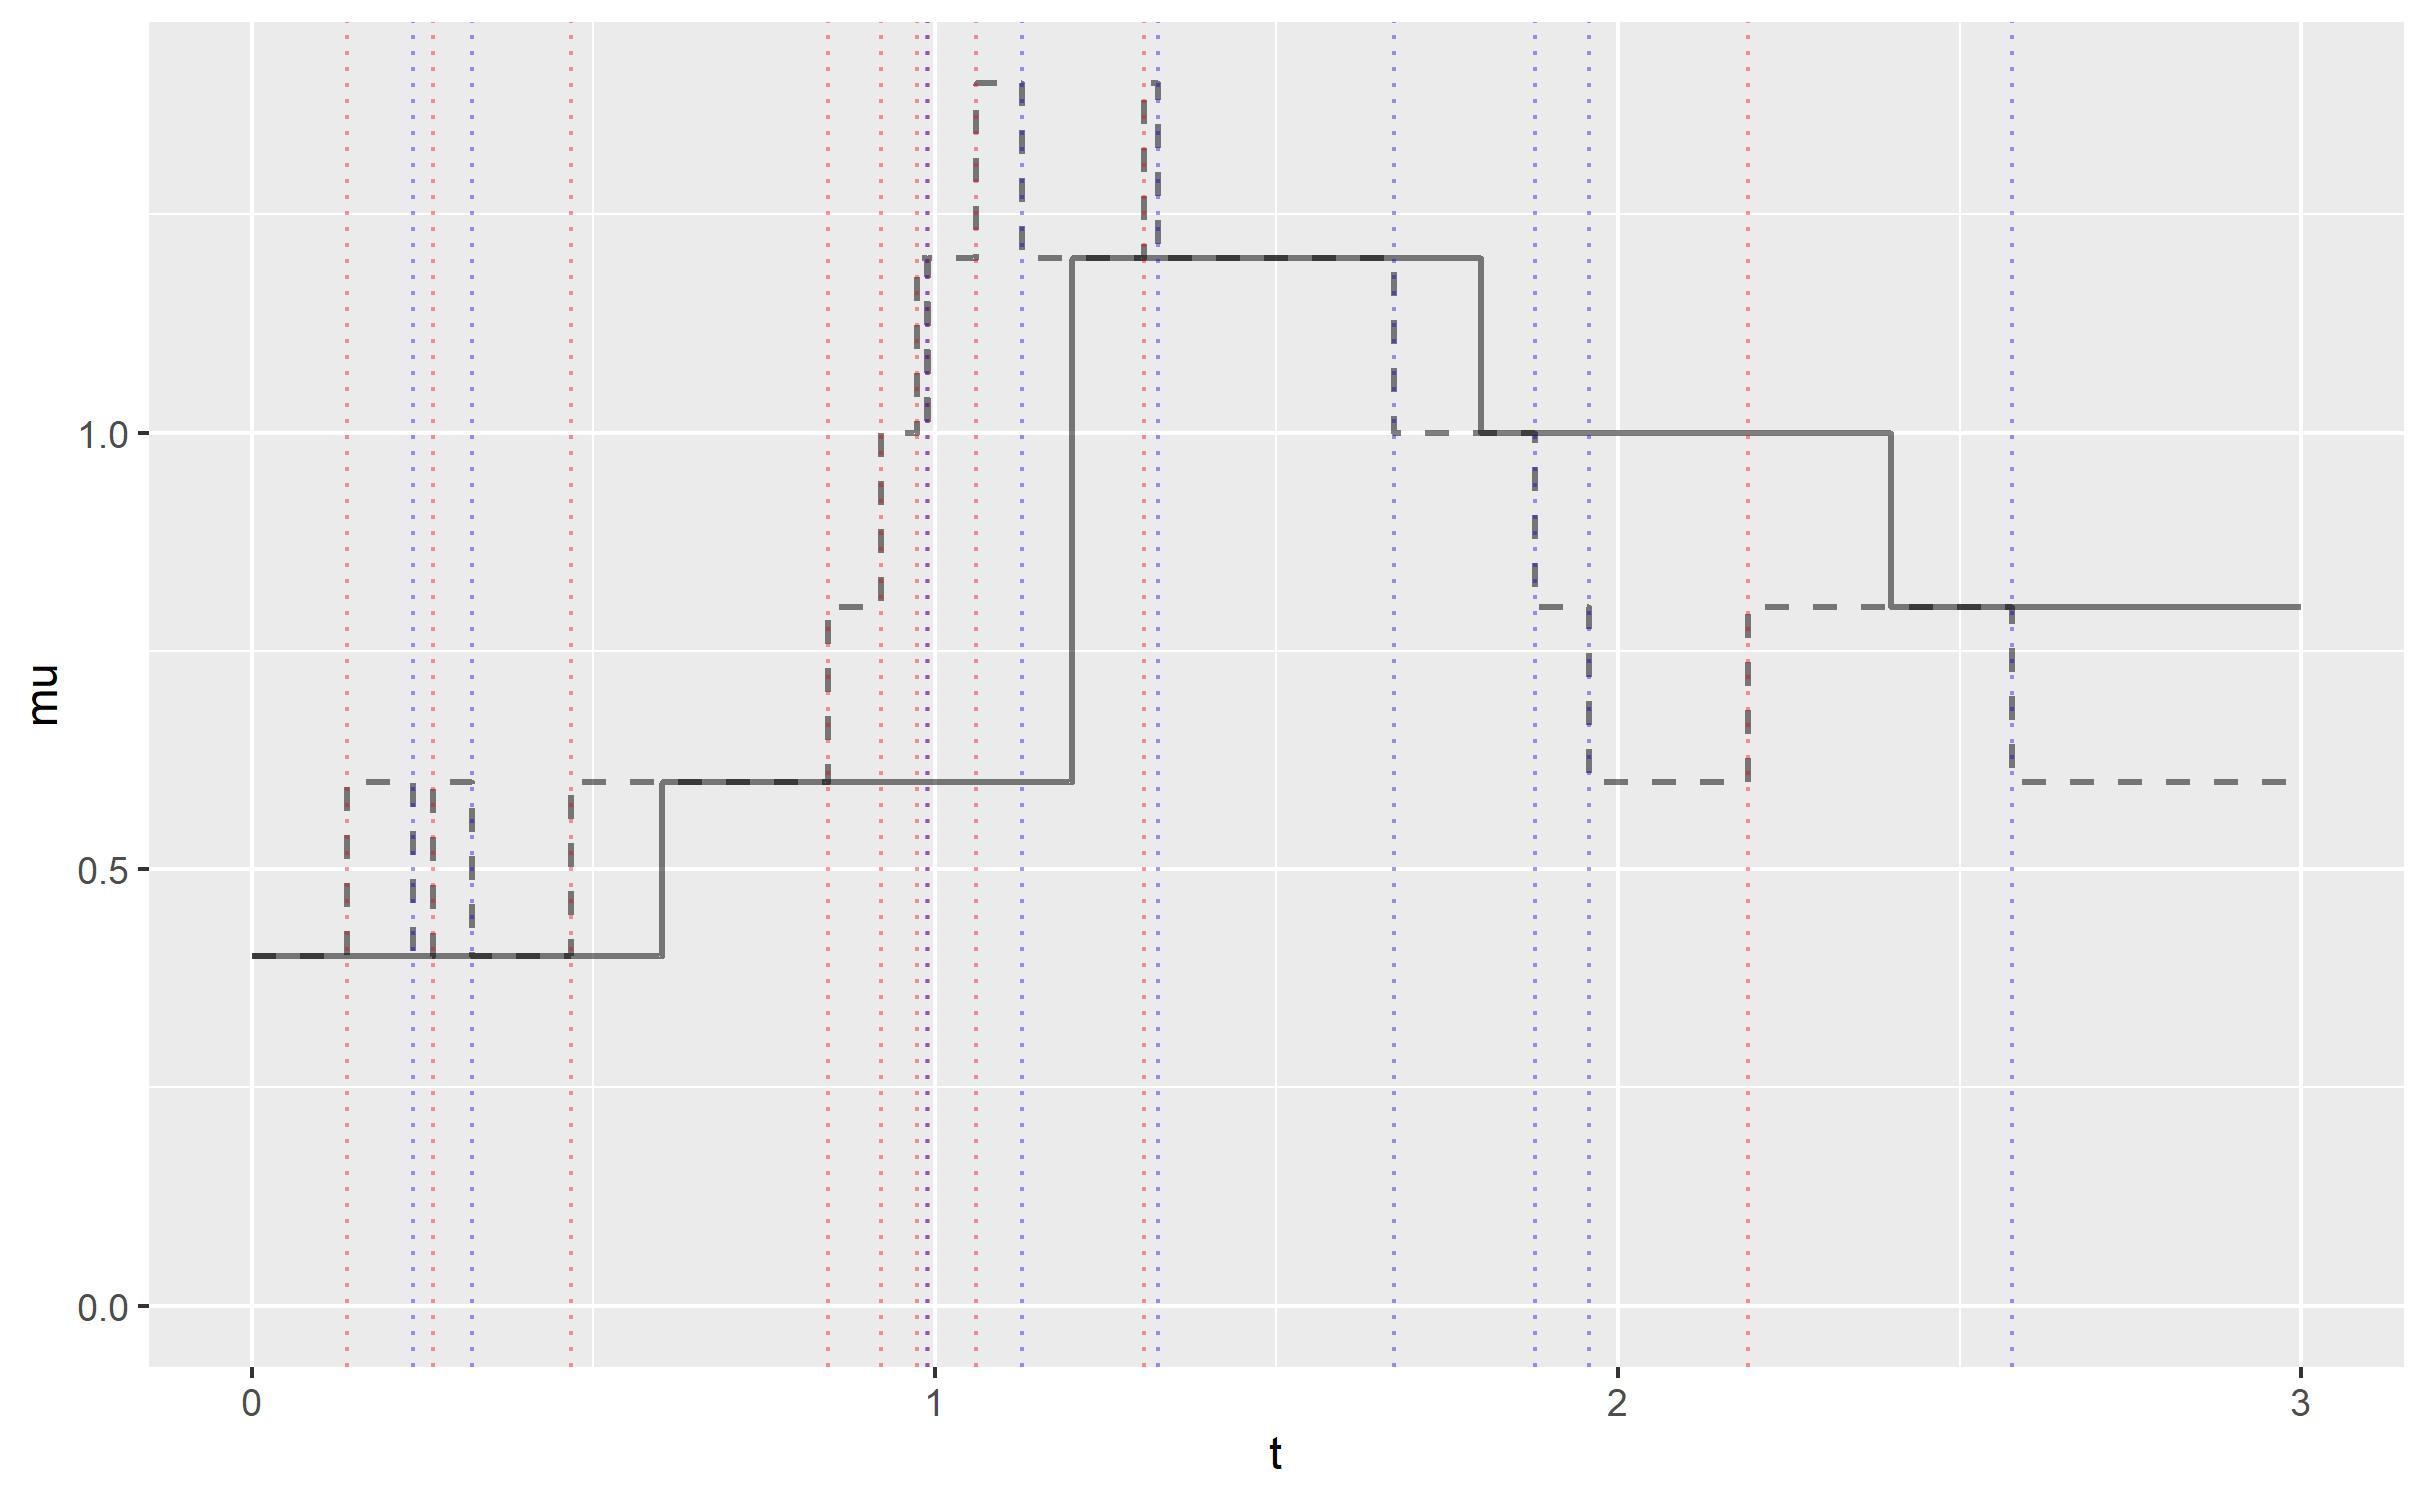
\includegraphics[scale = 0.6]{infection_rate_SIR_PDSIR.jpg}
		\caption{Infection dynamics of the SIR (dashed line) and PD-SIR (solid line) processes in a small population ($(S(0), I(0)) = (10,2)$) with $\beta=1$. The resetting schedule of the PD-SIR is $r_{0:3}=(0.0.2, 0.4, 0.6)$.
		The vertical dotted lines indicate the infection (red) and removal (blue) times.}
		\label{fig:mu}
	\end{figure}
	
	Now, by letting the resetting schedule $r_{0:L}$ coincide with the observation schedule $t_{0:K}$,
	$$L = K, \text{ and } r_k = t_k, \quad k=1,\dots,K,$$
	we can straightforwardly simulate realizations from the PD-SIR process conditionally on the observations $I_{1:K}$. By construction, under the PD-SIR model the population of susceptible individuals $S(t)$ follows a linear death process during each interval with death rate $\mu_k = \beta I(t_{k-1})$. Generating event times from a linear death process conditionally on the number of events happening by a certain time can be done extremely efficiently as shown by the following theorem whose proof is presented in Appendix \ref{app:ldp}.
	
	\begin{theorem}
		\label{theo:ldp}
		Consider a linear death process with death rate $\mu$ and let $d_{1:N} \in (t_l, t_u]$ be the times of the $N$ deaths occurring between times $t_l$ and $t_u$. Then 
		$$d_j \,{\buildrel d \over =}\, X_{(j)}, \quad j = 1, \dots, N$$
		where $X_{(j)}$ is the $j^{\text{th}}$ order statistics of $N$ i.i.d.\ random variables following a truncated exponential distribution with rate $\mu$, lower bound $t_l$ and upper bound $t_u$.
	\end{theorem}
	
	We can use this result to generate latent data  $\z = \left\lbrace (z^I_i, z^R_i)\right\rbrace_{i=1}^{n}$ compatible with $\Y = I_{1:K}$ from the PD-SIR process as follows. For each time interval $[t_{k-1}, t_k)$, we compute $\mu_k = \beta I(t_{k-1})$ and $U_k = I(0) + \sum_{l=1}^{k-1} I_l$, the cumulative number of infections that happened before $t_{k-1}$. The index set $\mathcal{I}_k = \{U_k + 1, \dots, U_k + I_k\}$ therefore denotes the $I_k$ individuals infected during the $k$th interval. Note that $I(t_{k-1})$ only depends on past events and can therefore be computed given the PD-SIR process up to time $t_{k-1}$. Algorithm \ref{alg:PD-SIR} provides a simple recursion to compute this variable efficiently. For $j \in \mathcal{I}_k$, following Theorem \ref{theo:ldp}, we sample the infection times $z^I_j$ from $\TruncExp(\mu_k; t_{k-1}, t_k)$, a truncated exponential distribution with rate $\mu_k$ bounded between $t_{k-1}$ and $t_k$ from which can efficiently be done with the inverse CDF method. For the same indices $j$, we then generate the removal times $z^R_j$ from the removal dynamics of the SIR. To accomplish this, we sample the removal time of individual $j$ from the mixed distribution
	$$(1 - p_j) \delta_{\infty} + p_j \TruncExp(\gamma; z^I_j, t_{end})$$
	placing point mass $(1 - p_j)$ at $\infty$ and continuous mass on $(z^I_j, t_{end}]$,
	where $\delta_{\infty}$ corresponds to the Dirac distribution with mass $1$ on the element $\infty$,
	$$p_j = 1 - \exp\{-\gamma (t_{end} - z^I_j)\} = P(z^R_j < t_{end} | z^I_j)$$
	is the cumulative distribution function of an exponential distribution with rate $\gamma$, % and corresponds to the probability that particle $j$ is removed before $t_{end}$ given that it was infected at time $z^I_j$,
	. By construction, this scheme generates latent data from the PD-SIR process that are compatible with the observed data. Algorithm \ref{alg:PD-SIR} provides a summary of the procedure in pseudo-code.
	
	\begin{algorithm}
		\caption{Generating a PD-SIR process conditionally on discretely observed infection incidence counts $I_{1:K}$}
		\label{alg:PD-SIR}
		\begin{algorithmic}
			\REQUIRE $I_{1:K}, \theta = (\beta, \gamma)$, $I(0)$
			\FOR {$j = 1, \dots, I(0)$}
			\STATE $z^I_j \leftarrow 0$ (by the memoryless property of the exponential distribution).
			\STATE $p_j \leftarrow 1 - \exp\{-\gamma (t_{end} - 0)\}$
			\STATE $z^R_j \sim (1 - p_j) \delta_\infty + p_j \TruncExp(\gamma, 0, t_{end})$
			\ENDFOR
			
			\FOR {$k = 1, \dots, K$}	
			\STATE $\mu_k \leftarrow \beta I(t_{k-1})$
			\STATE $X_{1 : I_k} \sim \TruncExp(\mu_k, t_{k-1}, t_k)$ i.i.d.\
			\STATE $U_k \leftarrow I(0) + \sum_{l=1}^{k-1} I_l$
			\STATE $\mathcal{I}_k \leftarrow (U_k + 1, \dots, U_k + I_k)$
			
			\FOR {$j \in \mathcal{I}_k$}
			\STATE $z^I_j \leftarrow X_{(j)}$ (infection times)
			\STATE $p_j \leftarrow 1 - \exp\{-\gamma(t_{end} - z^I_j)\}$
			\STATE $z^R_j \sim (1 - p_j) \delta_\infty + p_j \TruncExp(\gamma, z^I_j, t_{end})$ (removal times)
			\ENDFOR
			\STATE $R_k \leftarrow \#\{i:\tau^R_i \in (t_{k-1}, t_k]\}$ (number of removals in the $k^{\text{th}}$ interval)
			\STATE $I(t_k) \leftarrow I(t_{k-1}) + I_k - R_k$
			\ENDFOR
		\end{algorithmic}
	\end{algorithm}
	
	The density $q$ of the PD-SIR process can therefore be written as
	\begin{alignat*}{3}
		q(\z|\theta) & = && \prod_{k=1}^K \prod_{j\in\mathcal{I}_k} \TruncExp(z^I_j; \mu_{k}, t_{k-1}, t_{k}) \\
		& && \times \prod_{i=1}^{n} \left( 1 - p_i \right)^{\mathbf{1}(z^R_i = \infty)} \left( p_i \TruncExp(z^R_i; \gamma, z^I_i, t_{end}) \right)^{\mathbf{1}(z^R_i \le t_{end})} \\
		& = && \prod_{k=1}^K \prod_{j\in\mathcal{I}_k} \TruncExp(z^I_j; \mu_{k}, t_{k-1}, t_{k}) \\
		& && \times \prod_{i=1}^{n} \left( 1 - p_i \right)^{\mathbf{1}(z^R_i = \infty)} \left( p_i \TruncExp(z^R_i; \gamma, z^I_i, t_{end}) \right)^{\mathbf{1}(z^R_i \le t_{end})}
	\end{alignat*}
	where %$\mu_k = \beta I(t_{k-1})$ and
	$$\TruncExp(x; \mu, l, u) = \dfrac{\mu \exp\{-\mu x\}}{\exp\{-\mu l\} - \exp\{-\mu u\}}, \quad x \in (l, u)$$
	denotes the density of a truncated exponential distribution with parameters as notated previously.
	
	\subsection{Quality of Approximation}
	\label{sec:qua}
	% Outline: spaghetti plot, compare distribution of a particular infection time under SIR v approximation process (plot density and compute KS distance).
	
	Since the proposal for the latent data is independent from the current configuration of the latent data, the efficiency of the DA-MCMC algorithm to explore the latent space directly depends on how similar the surrogate process is to the target process. The Markov chain will have good mixing properties if the PD-SIR process is a close approximation of the SIR process. The PD-SIR process only differs from the SIR process in its infection dynamics, the removal dynamics being identical in the two processes. Figure \ref{fig:comparison} compares the trajectories of the compartments $S$, $I$ and $R$ of a SIR process of moderate size ($(S(0) = 1000, I(0), R(0)) = (1000, 10, 0)$ with $(\beta, \gamma) = (0.003, 1)$ and $t_{end} = 6$) and those of four PD-SIR processes constrained to be compatible with the observed incidence data $I_{1:K}$ from the SIR process for $K \in \{5, 10, 50, 1,000\}$. We see that the PD-SIR is qualitatively close to the SIR, even for small values of $K$. Unsurprisingly, the quality of the approximation improves as $K$ increases.
	% In the limit as $K \rightarrow \infty$, the infection times are effectively known.
	The fact that the PD-SIR is a faithful approximation of the SIR leads to a relatively high acceptance rate in the Metropolis-Hastings step for the latent data. As a result, our algorithm frequently makes larger jumps in the high-dimensional latent space and therefore explores it more efficiently.
	%Moreover, even though the latent spaces are generated from an approximation of the SIR process, the Metropolis-Hastings step ensures that the Markov chain converges to the posterior distribution of the parameters under the SIR model; in other words, the inference is exact. 
	
	\ram{Piece-wise linear trajectory of S compartment comes from the fact that it follows a linear death process with piece-wise constant rate.}
	
	\begin{figure}
		\centering
		\begin{subfigure}[b]{0.49\textwidth}
			\centering
			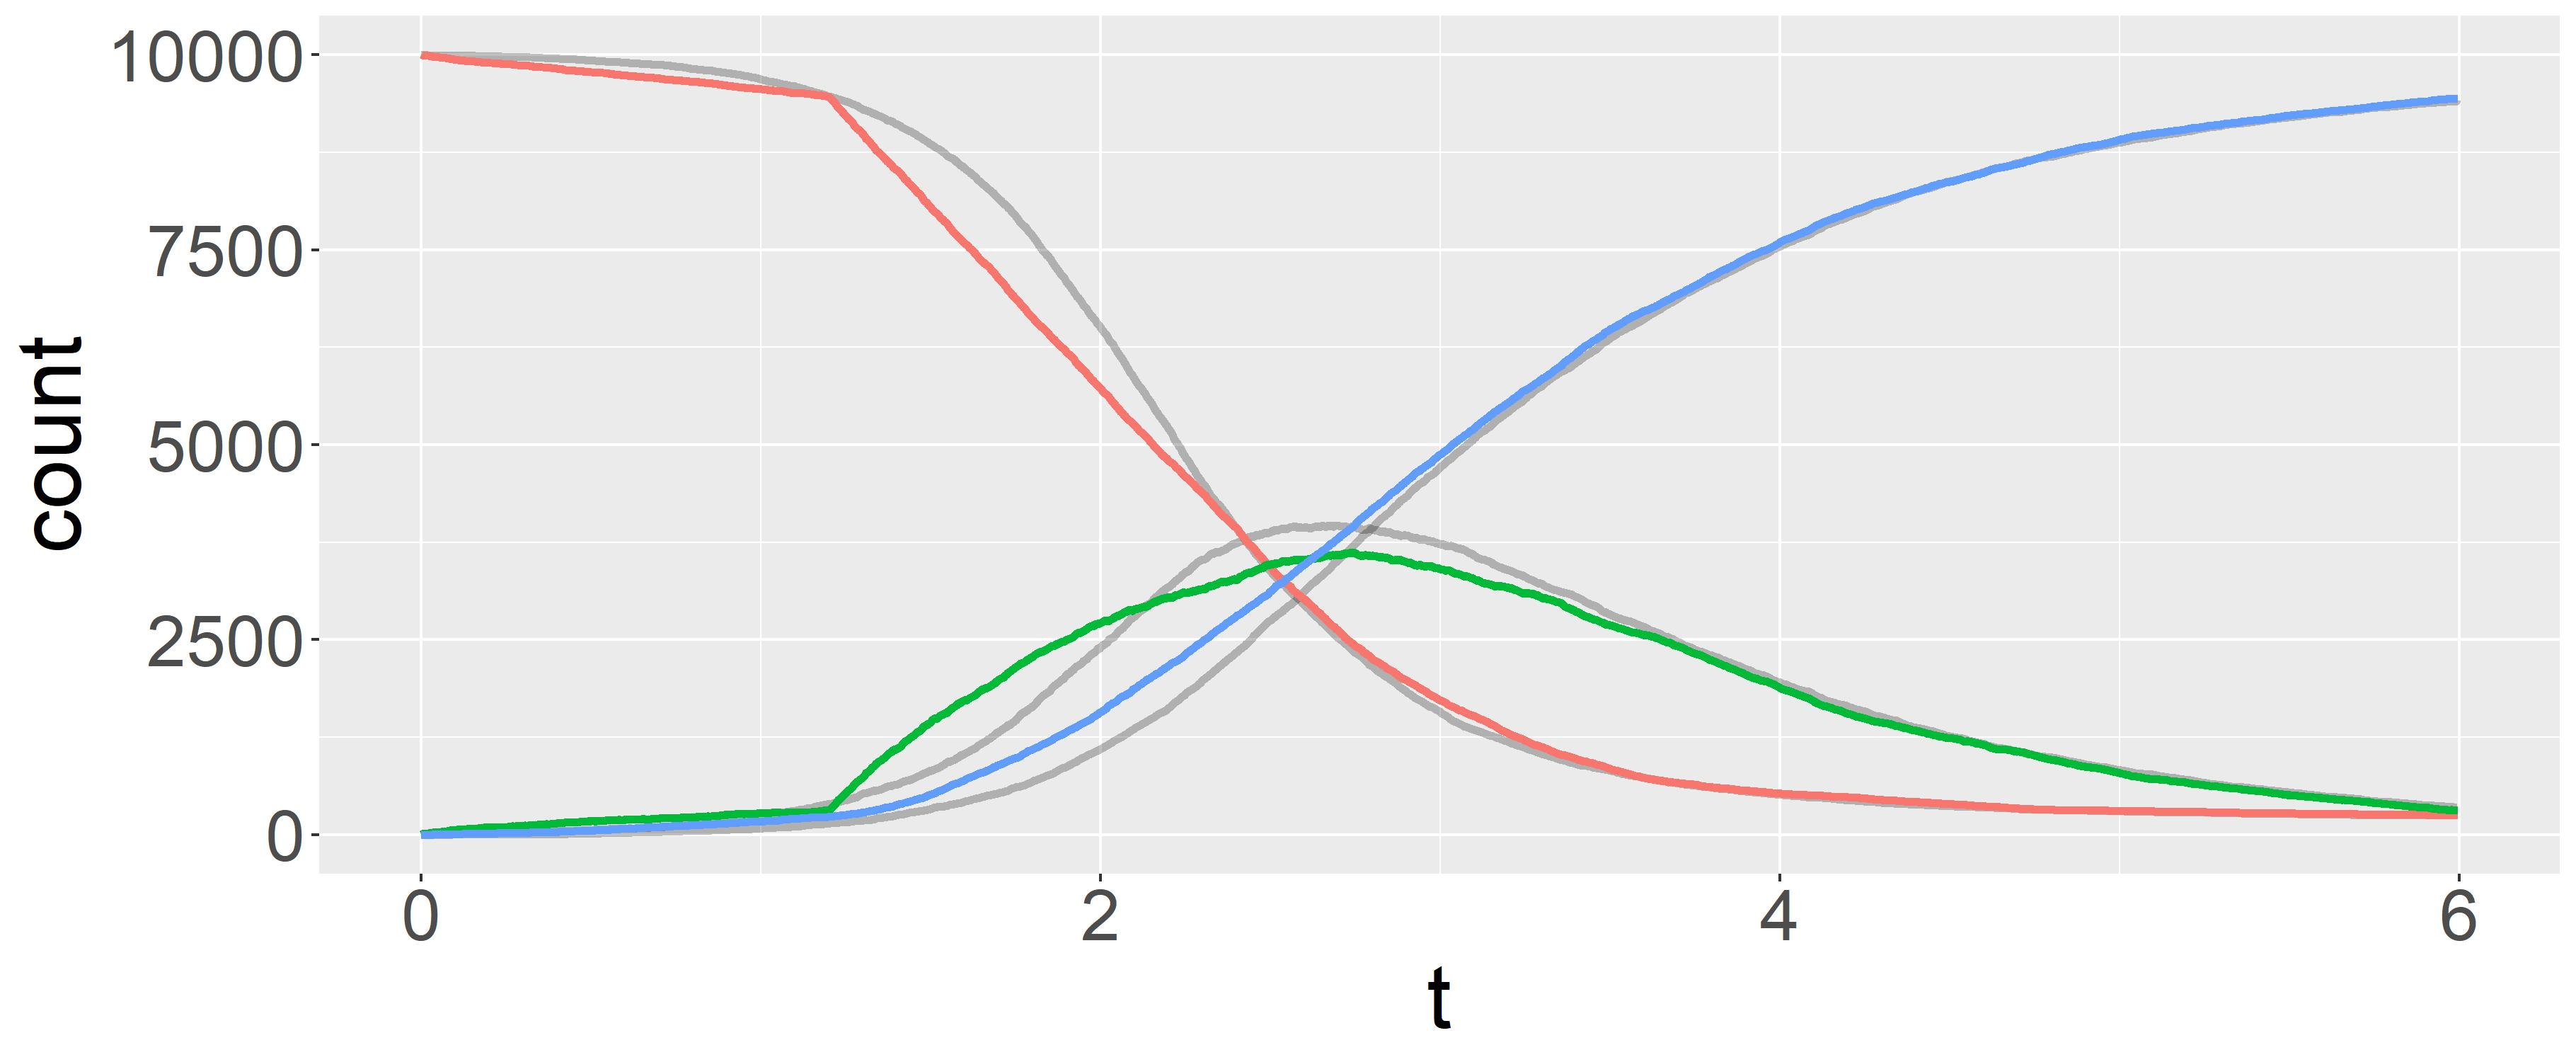
\includegraphics[width=\textwidth]{E2_K5}
			\caption{$K = 5$}
			\label{fig:comparison_RD_SIR_K5}
		\end{subfigure}
		\hfill
		\begin{subfigure}[b]{0.49\textwidth}
			\centering
			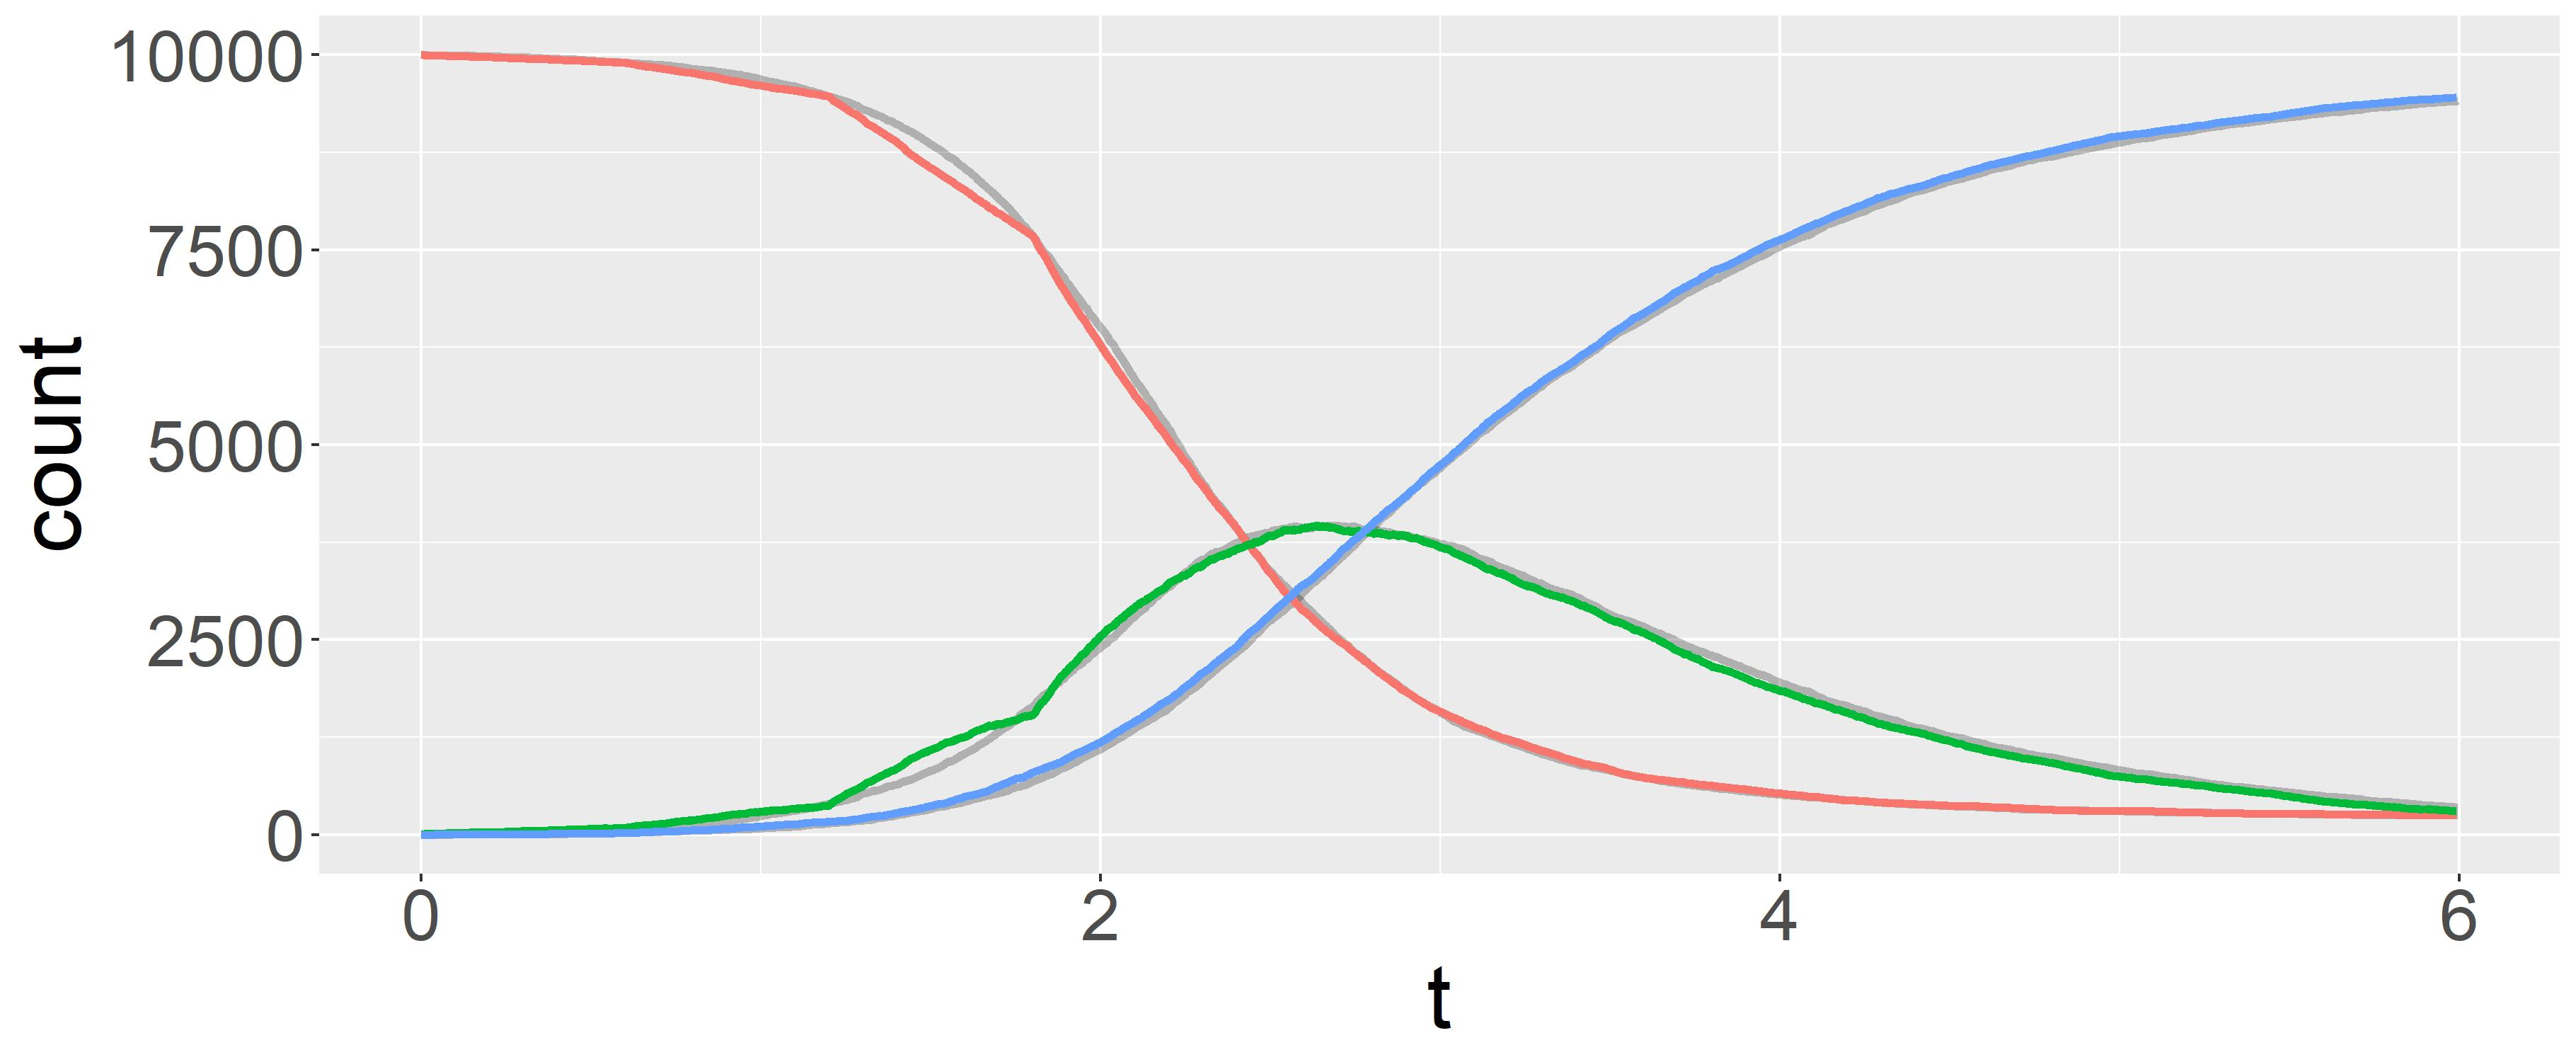
\includegraphics[width=\textwidth]{E2_K10}
			\caption{$K = 10$}
			\label{fig:comparison_RD_SIR_K10}
		\end{subfigure}
		\\
		\begin{subfigure}[b]{0.49\textwidth}
			\centering
			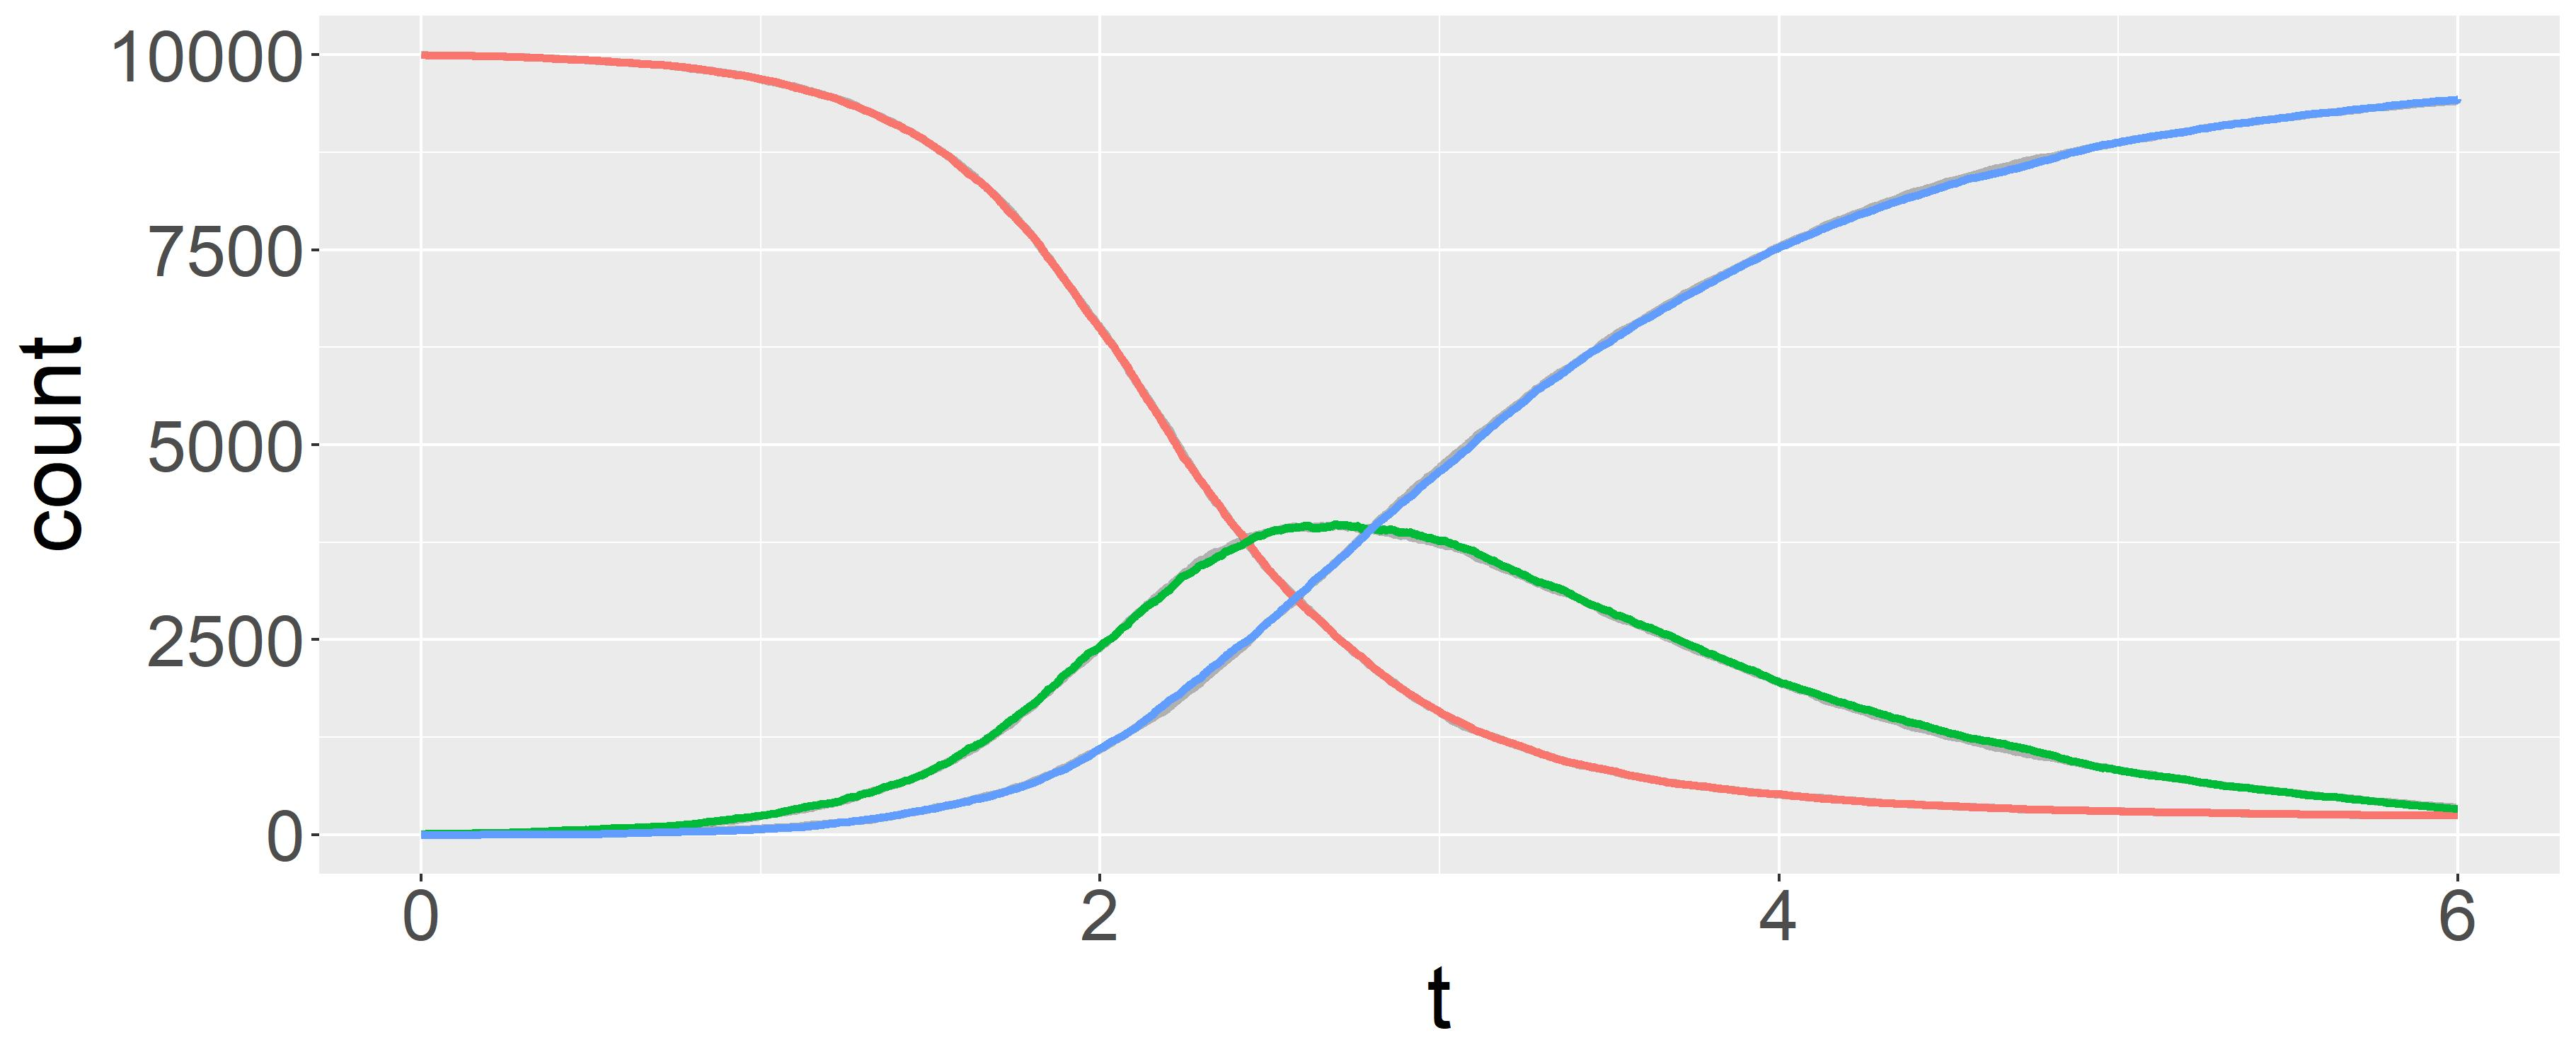
\includegraphics[width=\textwidth]{E2_K50}
			\caption{$K = 50$}
			\label{fig:comparison_RD_SIR_K50}
		\end{subfigure}
		\hfill
		\begin{subfigure}[b]{0.49\textwidth}
			\centering
			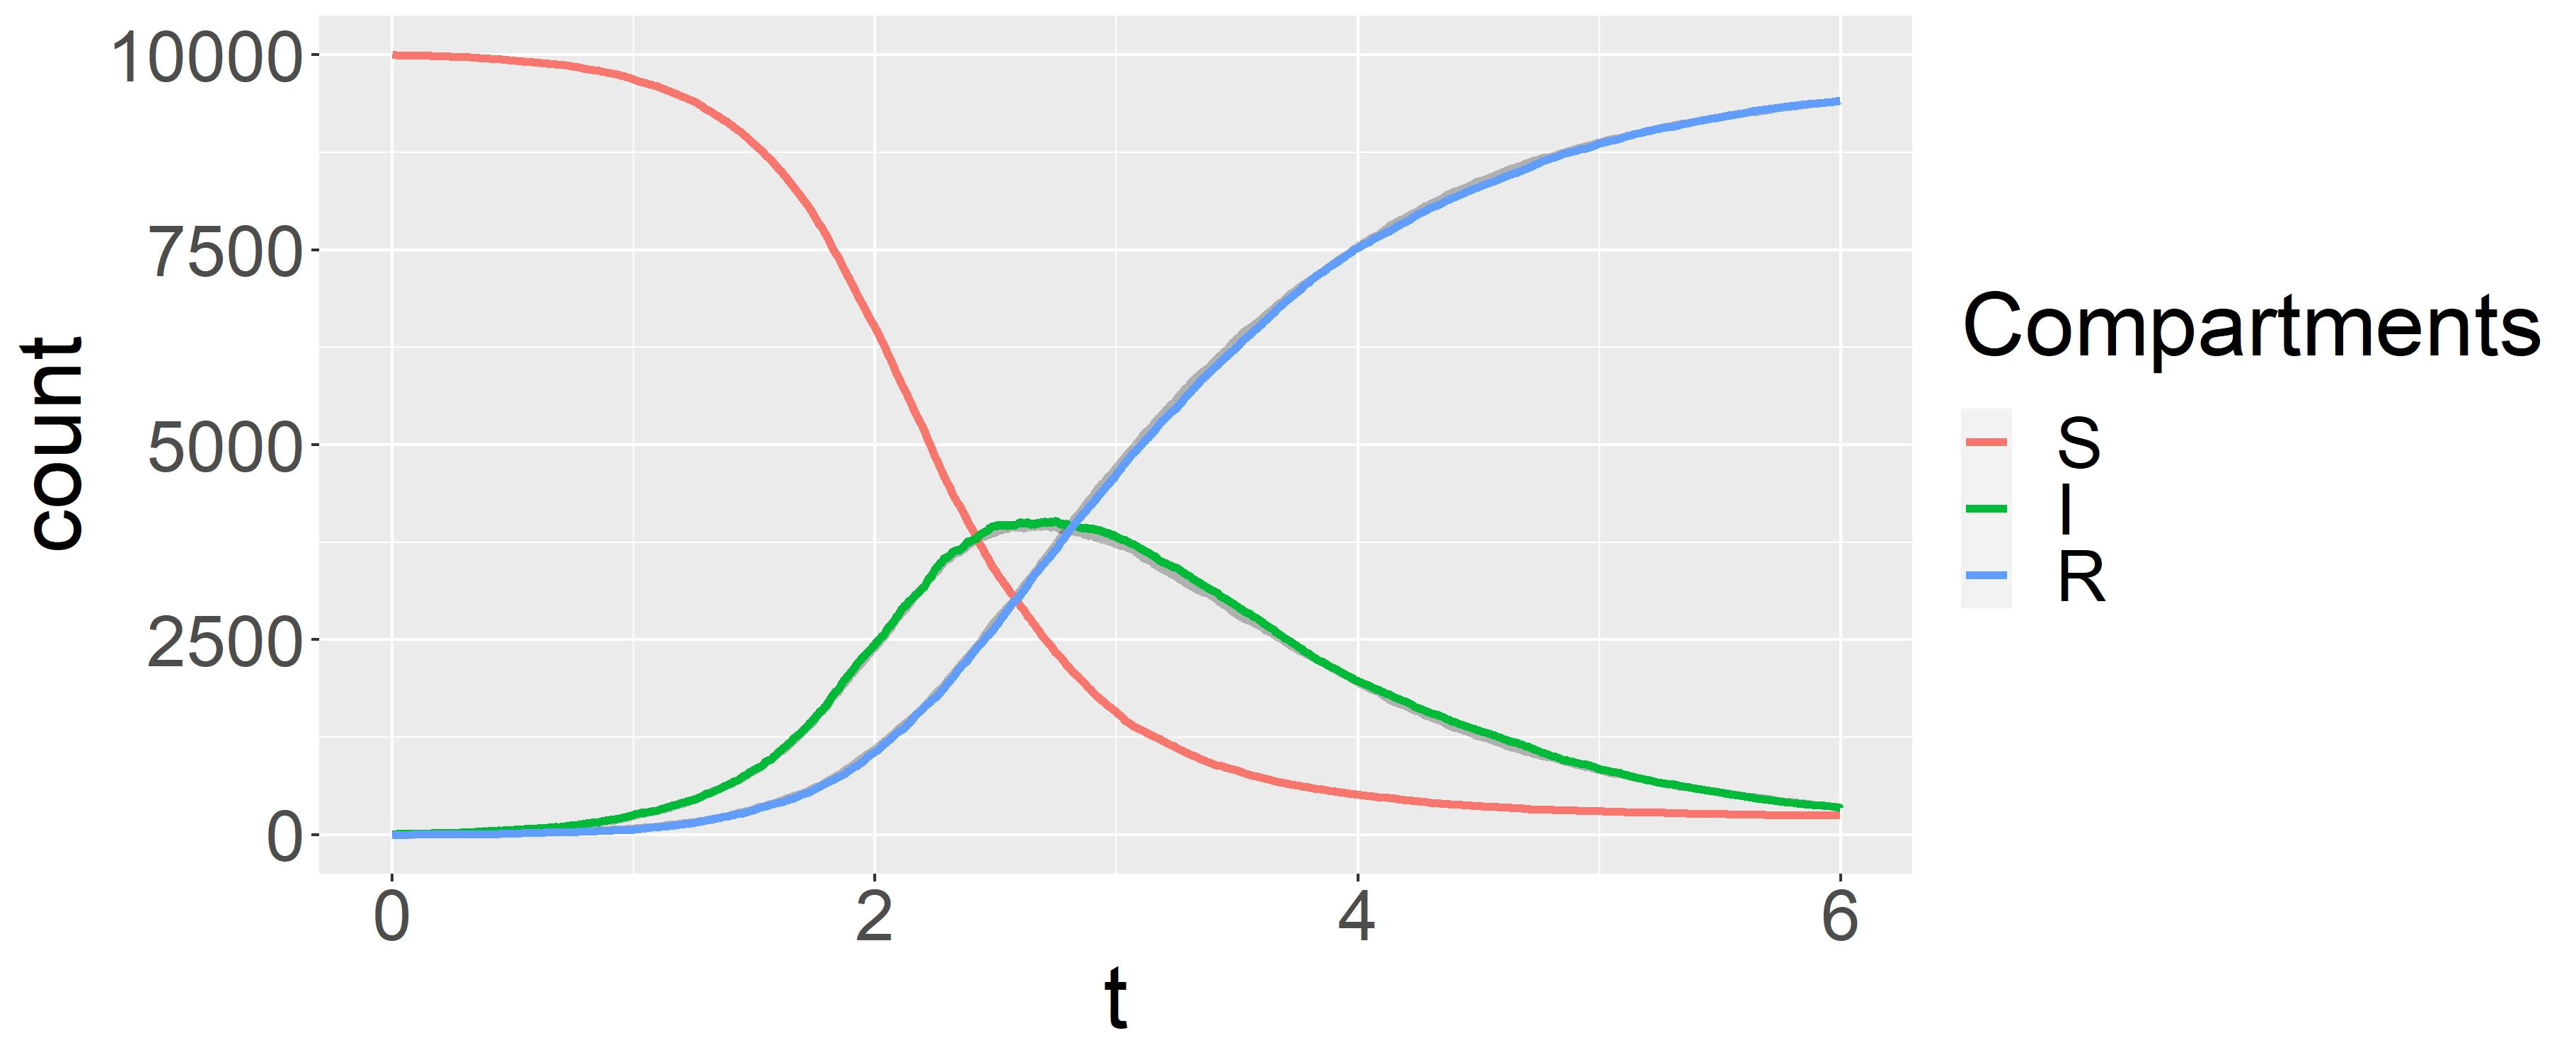
\includegraphics[width=\textwidth]{E2_K1000}
			\caption{$K = 1000$}
			\label{fig:comparison_RD_SIR_K1000}
		\end{subfigure}
		\caption{Trajectories of the compartments $S$, $I$ and $R$ in a SIR (in colors) and PD-SIR processes (in grey) with the same infection incidence data $T_{1:K}$.}
		\label{fig:comparison}
	\end{figure}
	\smallskip
	
	The following characteristics of our DA-MCMC algorithm are worth noting.
	First, initializing the Markov chain only requires setting $\theta^{(0)} = (\beta^{(0)}, \gamma^{(0)})$ since $\Z^{(0)}$ can be generated from the PD-SIR process conditionally on $\theta^{(0)}$ and $\Y$ alone.
	Second, since the PD-SIR closely approximates the SIR model, the acceptance rate in the Metropolis-Hastings step for the latent data is relatively high. For large population, however, the acceptance rate may be too low, thereby hindering the mixing of the Markov chain. To address this issue, we propose to update the event times of only a fraction $0<\rho\le 1$ of the individuals in the population; that is, in the Metropolis-Hastings step we only update the infection and removal times of $\lfloor\rho (S(0)+I(0))\rfloor$ individuals chosen randomly.
	Smaller values for $\rho$ result in smaller jumps in the latent space and a larger acceptance rate, which may lead to better mixing in certain cases.
	Third, if all event times are updated ($\rho = 1$), then the proposed and current latent data are independent conditionally on the current values of the parameters: $\Z^{(k-1)} \perp \Z^* | \theta^{(k)}$. This contrasts with existing DA-MCMC algorithms which only update a small fraction of the latent data per iteration.
	%Fourth, since the latent data are generated from a process that only resembles the SIR model, we ensure that the Markov chain converges to the correct distribution $\pi(\theta, \Z|\Y)$ by proposing and accepting the latent data according to a Metropolis-Hastings scheme. This results in exact Bayesian inference targeting the posterior distribution under the original SIR model.
	%Fifth, 
	Fourth, not only is proposing latent data from the RD-SIR process extremely fast since all random variables can be generated via the inverse-CDF method, but ensuring that these data are compatible with the observed data can be done at no additional cost, making the proposal scalable to large outbreaks.
	Finally, we show in the following section that the algorithm generates a Markov chain that is \textit{uniformly ergodic}, the strongest form of ergodicity for a Markov chain \cite{Tierney.1994}. %The proof of this result is provided in Appendix \ref{app:uni}.
	% our DA-MCMC only requires I(0), not S(0).
	
	\jx{We may insert a brief note explicitly contrasting with previous single-site RJMCMC work, giving a bit of intuition why we are able to avoid that change of space, and this could be a natural place to put it. Then, they also have a little more context for the experiment you've since added} 
	
	\subsection{Uniform Ergodicity}
	
	It is straightforward to show that the Markov chain $\{(\theta^{(m)}, \z^{(m)})\}_m$ is harris ergodic and converges to the target posterior distribution $\pi(\theta, \z|\Y)$. For any $\pi$-integrable function $g$, the estimator
	$$\bar{g}_m := \frac{1}{m} \sum_{i=0}^{m-1} g(\theta^{(m)}, \z^{(m)})$$
	is therefore consistent for $E_\pi g$, regardless of the starting values of the chain. A Markov chain is uniformly ergodic if for some finite $M$ and positive constant $r<1$ the $n$-step transition kernel $P^n$ satisfies
	$$
	\Vert P^n(x,.)-\pi(.)\Vert_{TV} \le M r^n, \forall x \in \chi
	$$
	where $\Vert \mu \Vert_{TV}$ denotes the total variation norm of the measure $\mu$.
	Uniform ergodicity ensures the existence of a Central Limit Theorem for $\bar{g}_m$ whenever $E_\pi |g|^2 < \infty$ (ref), that is,
	$$\sqrt{m}(\bar{g}_m - E_\pi g) \Rightarrow N(0, \sigma^2)$$
	for some positive, finite $\sigma^2$. Furthermore, uniform ergodicity implies that the batch means and spectral variance estimators of $\sigma^2$ are consistent (ref).
	
	
	%First, the Markov chain  $\{(\theta^{(m)}, \z^{(m)})\}_m$ is Harris recurrent and converges to the target posterior distribution. Indeed, by construction, the joint posterior density $\pi(\theta, \z|\Y)$ is invariant for the Gibbs kernel $P_\theta$ and the Metropolis-Hastings kernel $P_\z$ and the density of the composite kernel $P = P_\theta P_\theta$ is strictly positive, implying that the chain is aperiodic and $\pi$-irreducible. Together with the existence of an invariant distribution, $\pi$-irreducibility implies that the chain is positive Harris recurrent.
	
	Toward establishing uniform ergodicity of our DA-MCMC algorithm, we will show that the state space $\chi = \chi_{\theta}\times\chi_{\z}$ of the Markov chain $\{(\theta^{(m)}, \z^{(m)})\}_m$ is a \textit{small set} for the transition kernel $P$. That is, there exists a probability measure $\nu$ on the $\sigma$-algebra $\sigma(\chi)$ such that
	$$\beta \nu(.) \le P^m(x,.), \forall x\in \chi.$$
	for some constants $m \ge 1$ and $\beta > 0$.
	By Proposition 2 in \cite{Tierney.1994}, this implies that the Markov is uniformly ergodic. 
	
	To derive this result, we will make use of three lemmas. The appendix contains a detailed a proof of the latter two.
	\rm{Figures for lemma 3.1 and 3.2?}
	
	% Gamma 1
	\begin{lemma}
		\label{pro:ga1}
		Let $Ga(x;a,b)$ denote the density of the gamma distribution with shape $a$ and rate $b$ evaluated at $x$. Then
		\begin{equation}
			\label{eq:ga1}
			\inf_{0\le \beta\le B} Ga(x;a,b+\beta) = 
			\begin{cases}
				Ga(x;a,b), & x<x_a^* \\ Ga(x;a,b+B), & x\ge x_a^*
			\end{cases}
		\end{equation}	
		where $x_a^*=\frac{a}{B}\log\left( 1+\frac{B}{b}\right) $. Moreover,
		\begin{equation}
			\label{eq:ga2}
			\inf_{0\le \alpha\le A} Ga(x;a+\alpha,b) = 
			\begin{cases}
				Ga(x;a,b), & x>x_b^* \\ Ga(x;a+A,b), & x\le x_b^*
			\end{cases}
		\end{equation}
		where $x_b^*=\frac{1}{b}\left[ \frac{\Gamma(a+A)}{\Gamma(a)}\right]^{1/A} $.
	\end{lemma}
	\begin{proof}
		Equation \ref{eq:ga1} is proven in Jones, Hobert (2004). For Equation \ref{eq:ga2}, note that $x_b^*$ is the only positive solution to $Ga(x;a,b) = Ga(x;a+A,b)$. Now, for all $0<x\le x_b^*$ and all $0\le\alpha\le A$, we have
		\begin{align*}
			\frac{Ga(x;a+A,b)}{Ga(x;a+\alpha,b)}
			& = b^{A-\alpha}x^{A-\alpha} \frac{\Gamma(a+\alpha)}{\Gamma(a+A)} \\
			& \le b^{A-\alpha}\left(\frac{1}{b}\left[ \frac{\Gamma(a+A)}{\Gamma(a)}\right]^{1/A} \right)^{A-\alpha} \frac{\Gamma(a+\alpha)}{\Gamma(a+A)} \\
			& = \left[ \frac{\Gamma(a+A)}{\Gamma(a)}\right]^{(A-\alpha)/A} \frac{\Gamma(a+\alpha)}{\Gamma(a+A)} \\
			& = \left( \frac{\Gamma_{a,a+A}}{\Gamma_{a+\alpha, a+A}}\right)^{A-\alpha} \\
			& \le 1,
		\end{align*}
		where $\Gamma_{d,e} = \left( \frac{\Gamma(e)}{\Gamma(d)} \right)^{\frac{1}{e-d}}$ is a geometric average,
		and where the last inequality holds because $\Gamma_{a,a+A}\le\Gamma_{a+\alpha, a+A}$.
		The case $x>x_b^*$ can be shown similarly.
	\end{proof}
	
	
	Lemma \ref{pro:ga1} can be used to minorize a gamma density of the form
	\begin{equation}
		\label{eq:ga}
		Ga(x;a+\alpha,b+\beta) = \frac{(b+\beta)^{a+\alpha}}{\Gamma(a+\alpha)}x^{a+\alpha-1}\exp\{-x(b+\beta)\}, \quad 0\le\alpha\le A, 0\le\beta\le B.
	\end{equation}
	over $\alpha$ and $\beta$ for each value of $x$. To this end, we establish the following technical lemma.
	\begin{lemma}	
		\label{pro:ga2}
		For a fix $x>0$, the density $Ga(x;a+\alpha,b+\beta)$ is minimized by $(\alpha, \beta) \in \{(A, 0), (0, B)\}$, the minimizing set of values depending on $x$. In particular,	
		$$\inf_{\begin{aligned}
				0\le \alpha\le A \\ 0\le \beta\le B
		\end{aligned}}Ga(x;a+\alpha,b+\beta) = 
		\begin{cases}
			Ga(x;a+A,b)                     , & x<x_a         \text{ or } x<x_{a+A}^* \vee x_b^*\\
			Ga(x;a,b+B)                     , & x_{a+A}^* < x \text{ or } x_a^* \wedge x_{b+B}^* < x\\
			\min\{Ga(x;a+A,b), Ga(x;a,b+B)\}, & x_a^* \wedge x_b^*\le x < x_{a+A}^* \vee x_{b+B}^*\\
		\end{cases}$$
	\end{lemma}
	The final lemma can be used to minorize truncated exponential densities.
	\begin{lemma}
		\label{pro:tru}
		$$\min_{0 \le \mu \le M} \TruncExp(x; \mu, l, u) = \TruncExp(x; M, l, u) $$
	\end{lemma}
	
	%\noindent
	We can now proceed with the proof of uniform ergodicity.
	% Uniform Ergodicity
	\begin{proposition}
		\label{pro:uni}
		The transition kernel $P = P_{\theta}P_{\z}$ of our DA-MCMC algorithm satisfies a minorization condition $M(1, \delta, \chi, \nu)$ and, as a result, is uniformly ergodic.
	\end{proposition}
	
	\begin{proof}
		First, note that the transition kernel $P$ is a composition of two kernels
		$$ P = P_{\theta} P_{\z}$$
		where the kernel $ P_{\theta}$ updates the parameters $\theta$ while keeping the latent data $\z$ fixed and $P_{\z}$ update $\z$ while keeping $\theta$ fixed. A one-step transition therefore corresponds to the following scheme 
		$$\x_1 = (\theta_1, \z_1) \rightarrow (\theta_2, \z_1) \rightarrow (\theta_2, \z_2) = \x_2.$$
		
		The kernel $P$ has a density $p$ with respect to the product measure $\mu = \lambda \mu_{\z}$ with $\lambda$ the Lebesgue measure on $\chi_{\theta}$, the space of $\theta$, and $\mu_{\z}$ a $\sigma$-finite measure on $\chi_{\z}$, the space of $\z$.
		\begin{align*}
			P(\x_1, d\x_2) 
			& = p(\x_1, \x_2) \mu(d\x_2) \\
			& = p((\theta_1, \z_1), (\theta_2, \z_2)) \lambda(d\theta_2)\mu_{\z}(d\z_2) \\
			& = p_{\theta}((\theta_1, \z_1), (\theta_2, \z_1)) p_{\z}((\theta_2, \z_1), (\theta_2, \z_2)) \mu_{\z}(d\z_2) \lambda(d\theta_2)
		\end{align*}
		where
		\begin{align*}
			p_{\theta}((\theta_1, \z_1), (\theta_2, \z_1))
			%	& = q_{\theta}((\theta_1, \z_1), (\theta_2, \z_1)) \alpha((\theta_1, \z_1), (\theta_2, \z_1)) \\
			& = \pi(\theta_2| \z_1) \\
			& = \pi(\beta_2|\z_1) \pi(\gamma_2|\z_1)
		\end{align*}
		is the density of the transition kernel $P_{\theta}$ with respect to $\lambda$ and corresponds to the product of the full conditional distributions of $\beta$ and $\gamma$ since the kernel $P_{\theta}$ is a Gibbs sampler, and
		\begin{align*}
			p_{\z}((\theta_2, \z_1), (\theta_2, \z_2))
			& = q_{\z}((\theta_2, \z_1), (\theta_2, \z_2)) \alpha((\theta_2, \z_1), (\theta_2, \z_2)) \\
			& = q(\z_2; \theta_2) \min\left\lbrace 1, \dfrac{\pi(\theta_2, \z_2)q(\z_1; \theta_2)}{\pi(\theta_2, \z_1)q(\z_2; \theta_2)} \right\rbrace \\
			& = \min\left\lbrace q(\z_2; \theta_2), \dfrac{\pi(\theta_2, \z_2)q(\z_1; \theta_2)}{\pi(\theta_2, \z_1)} \right\rbrace
		\end{align*}
		is the density of the transition kernel $P_{\z}$ with respect to $\mu_{\z}$ and corresponds to one step of the Metropolis-Hasting algorithm where a new configuration of the latent data $\z_2$ is proposed conditionally on the current value of the parameters $\theta_2$, but independently of the current configuration $\z_1$.
		
		To show that $\chi$ is a small state, it is sufficient to show that there exists a function $k$ such that
		$$p(\x_1, \x_2) \ge k(\x_2) > 0, \qquad \forall \x_1 \in \chi $$
		for all $\x_2 \in \chi$.
		The density $p$ 
		\begin{align*}
			p((\theta_1, \z_1), (\theta_2, \z_2))
			& = \min\left\lbrace \pi(\theta_2| \z_1)g(\z_2; \theta_2), \dfrac{\pi(\theta_2| \z_1) \pi(\theta_2, \z_2)}{\pi(\theta_2, \z_1)} g(\z_1; \theta_2) \right\rbrace \\
			& = \min\left\lbrace \pi(\theta_2| \z_1)g(\z_2; \theta_2), \dfrac{\pi(\theta_2, \z_2)}{\pi(\z_1)} g(\z_1; \theta_2) \right\rbrace \\
			%	& = \min\left\lbrace \pi(\theta_2| \z_1)g(\z_2; \theta_2),		\dfrac{			\frac{f(\theta_2, \z_1, Y)}{f(\z_1, Y)}			\frac{f(\theta_2, \z_2, Y)}{f(Y)}		}{\frac{f(\theta_2, \z_1, Y)}{f(Y)}} 		g(\z_1; \theta_2)\right\rbrace \\
			%	& = \min\left\lbrace \pi(\theta_2| \z_1)g(\z_2; \theta_2),		\dfrac{f(\theta_2, \z_2, Y)}{f(\z_1, Y)}		g(\z_1; \theta_2)\right\rbrace \\
			& = \min\left\lbrace \pi(\theta_2| \z_1)g(\z_2; \theta_2),
			\pi(\theta_2| \z_2)
			g(\z_1; \theta_2)\right\rbrace
		\end{align*}
		depends on $x_1 = (\theta_1, \z_1)$ only through the full conditional $\pi(\theta_2| \z_1)$ and the proposal density $g(\z_1; \theta_2)$.
		
		It therefore suffices to show that there exist functions $k_1$ and $k_2$ such that
		$$\pi(\theta| \z_1) \ge k_1(\theta) > 0 \qquad \text{and} \qquad  g(\z_1; \theta) \ge k_2(\theta) > 0.$$
		First, 
		\begin{align*}
			\pi(\theta| \z_1) 
			& = \pi(\beta| \z_1) \pi(\gamma| \z_1)  \\
			& = Ga(\beta; a_{\beta} + n_T, b_{\beta} + SI_1) Ga(\gamma; a_{\gamma} + {n_J}_1, b_{\gamma} + I_1) \\
			& \ge h_{\beta}(\beta) h_{\gamma}(\gamma) \\
			& = k_1(\theta) > 0
		\end{align*}
		where, by Proposition \ref{pro:ga1},
		$$h_{\beta}(\beta) = \begin{cases}
			Ga(\beta;a_{\beta}+n_T,b_{\beta}), & \beta<\frac{a_{\beta}+n_T}{t_{end}(n_T+I_0) n} \log \left( 1 + \frac{t_{end}(n_T+I_0) n}{b_{\beta}}\right) \\ Ga(x;a_{\beta}+n_T,b_{\beta}+n(n_T+I_0) t_{end}), & \text{else}
		\end{cases}$$
		since $n_T = \sum_k T_k$ is known and 
		$$SI_1 = \int_{0}^{t_{end}}S_1(t)I_1(t)dt \in [0, n (n_T+I_0) t_{end}];$$
		and, by Proposition \ref{pro:ga2},
		$$h_{\gamma}(\gamma) = \min\{
		Ga(\gamma;a_{\gamma}+n_T+I_0,b_{\gamma}), Ga(x;a_{\gamma},b_{\gamma}+(n_T+I_0) t_{end})\}
		$$
		since $0\le n_1^J \le n_T + I_0$ and
		$$I_1 = \int_{0}^{t_{end}}I_1(t)dt \in [0, (n_T+I_0) t_{end}].$$
		
		Second, each factor in
		\begin{align*}
			& g(\z_1; \theta) = \prod_{i=1}^{n_T} \TruncExp(z^T_i; \beta I_k, t_{k(i)-1}, t_{k(i)}) (1-p_i)^{1\{\z^J_i = \infty\}} (p_i \TruncExp(z^J_i; \gamma, z^T_i, t_{end}))^{1\{\z^J_i \le t_{end}\}}
		\end{align*}
		can be minorized as follows. First,
		\begin{align*}
			\TruncExp(z^T_i; \beta I_k, t_{k(i)-1}, t_{k(i)}) 
			& \ge \TruncExp(t_{k(i)}; \beta I_k, t_{k(i)-1}, t_{k(i)}) \\
			& \ge \TruncExp(t_{k(i)}; \beta (n_T + I_0), t_{k(i)-1}, t_{k(i)}),
		\end{align*}
		with the last inequality following from Proposition \ref{pro:tru}, second,
		$$1-p_i = \exp\{-\gamma (t_{end} - z^T_i)\} \ge \exp\{-\gamma (t_{end} - t_{k(i)-1})\},$$
		third,
		$$p_i \TruncExp(z^J_i; \gamma, z^T_i, t_{end}) = \Exp(z^J_i - z^T_i; \gamma)1(z^T_i < z^J_i \le t_{end}) \ge \Exp(t_{end} - t_{k(i) - 1}; \gamma)$$
		where the equality holds since $p_i = P(z^J_i \le t_{end}|z^J_i > z^T_i)$ is equal to the normalizing constant of the truncated exponential.
		
		Taken together, these inequalities give
		\begin{align*}
			g(\z_1; \theta)
			& \ge \prod_{i=1}^{n_T} \TruncExp(t_{k(i)}; \beta (I_0 + n_T), t_{k(i)-1}, t_{k(i)}) \min\{\exp\{-\gamma (t_{end} - t_{k(i) - 1})\}, \Exp(t_{end} - t_{k(i) - 1}; \gamma)\} \\
			& = k_2(\theta) > 0
		\end{align*}
		which completes the proof.
	\end{proof}
	
	
	
	The kernel 
	$$
	P_{\theta}((\theta_0, \z), (\theta_1, \z)) = Ga\left( \beta_1; a_{\beta} + n_I, b_{\beta} + \int_0^{t_{end}} S(t)I(t) dt\right) Ga\left( \gamma_1; a_{\gamma} + n_R, b_{\gamma} + \int_0^{t_{end}} I(t) dt\right) d\beta_1 d\gamma_1
	$$
	therefore corresponds to a Gibbs kernel where $n_I, n_R, \int S(t)I(t) dt, \int I(t) dt$ are sufficient statistics from the latent data $\z$
	
	\section{Performance on simulated and real epidemic data}
	\label{sec:per}
	
	\subsection{Simulation Study}
	\label{sec:sim}
	%Outline: (1) proof of concept, (1bis) coverage, (2) rho (3) single-site versus joint proposal
	
	We validate the convergence properties of the proposed DA-MCMC algorithm empirically via a suite of simulation studies. First, we assess the performance of the DA-MCMC algorithm in a medium-sized population of over $1000$ individuals. We simulate an epidemic from true parameters $(\beta, \gamma) = (0.0025, 1)$, which gives $R_0 = 2.5$, starting with $(S(0), I(0)) = (1000, 10)$ until time $t_{end} = 6$ when the outbreak has completed most of its course but is not over yet (see Figure \ref{fig:E1_trajectories}, where $I(t_{end}) = 55$). The numbers of infections in $K = 10$ time intervals of equal length are observed, corresponding to $I_{1:K} = (9, 14, 21, 42, 56, 121, 190, 162, 107, 73)$.	
	We use the conjugate prior distributions \ref{eq:pri} $\beta \sim Ga(0.001, 1)$ and $\gamma \sim Ga(1,1)$, which are only weakly informative.
	The Markov chain is initialized in a low density region at $(\beta^{(0)}, \gamma^{(0)}) = (\beta/10, \gamma/10) = (0.00025, 0.1)$, and we keep every tenth draw for storage reasons, and set $\rho = 0.2$ so that the trajectories of $\lfloor\rho (S(0)+I(0))\rfloor = 202$ individuals are updated in each Metropolis-Hastings step. The algorithm takes less than $30$ minutes to generate $1$ million samples on a personal laptop. 
	
	Figure \ref{fig:E1_short_no_burn_gamma_tp} shows the traceplot of the parameter $\gamma$ for the first $10000$ iterations. We observe that the Markov chain quickly migrates from the low density region where it is initialized to the mode of the target distribution. Figures  \ref{fig:E1_burn_gamma_tp} and \ref{fig:E1_burn_gamma_acf}, which show the traceplot of $\gamma$ after a burn-in period of $10000$ iterations and its auto-correlation function, indicate that once the chain reaches the high density region it mixes well. The acceptance rate of the Metropolis-Hastings step is $0.21$.
	The posterior means of $\beta$, $\gamma$ and $R_0$ are respectively $0.00217$, $0.815$ and $2.75$, respectively based on $398$, $370$ and $438$ effective sample sizes. The $90\%$ credible intervals are $(0.00166, 0.00278)$, $(0.492, 1.19)$ and $(2.26, 3.45)$ and cover the true values of the parameters. To validate the uncertainty quantification of the posteriors under our DA-MCMC algorithm, we examine frequentist coverage properties of posterior credible intervals under $2000$ independently repeats of the experiment. Tables \ref{tab:coverage} provides the empirical coverage of the $90\%$ credible intervals for the parameters $\beta$, $\gamma$ and $R_0$ along with the average and variance of the posterior means. The algorithm has the appropriate coverage, suggesting that running the chain for $1$ million iterations is sufficient to approximate the posterior distribution of the parameters.
	
	\begin{figure}
		\centering
		\begin{subfigure}[b]{0.42\textwidth}
			\centering
			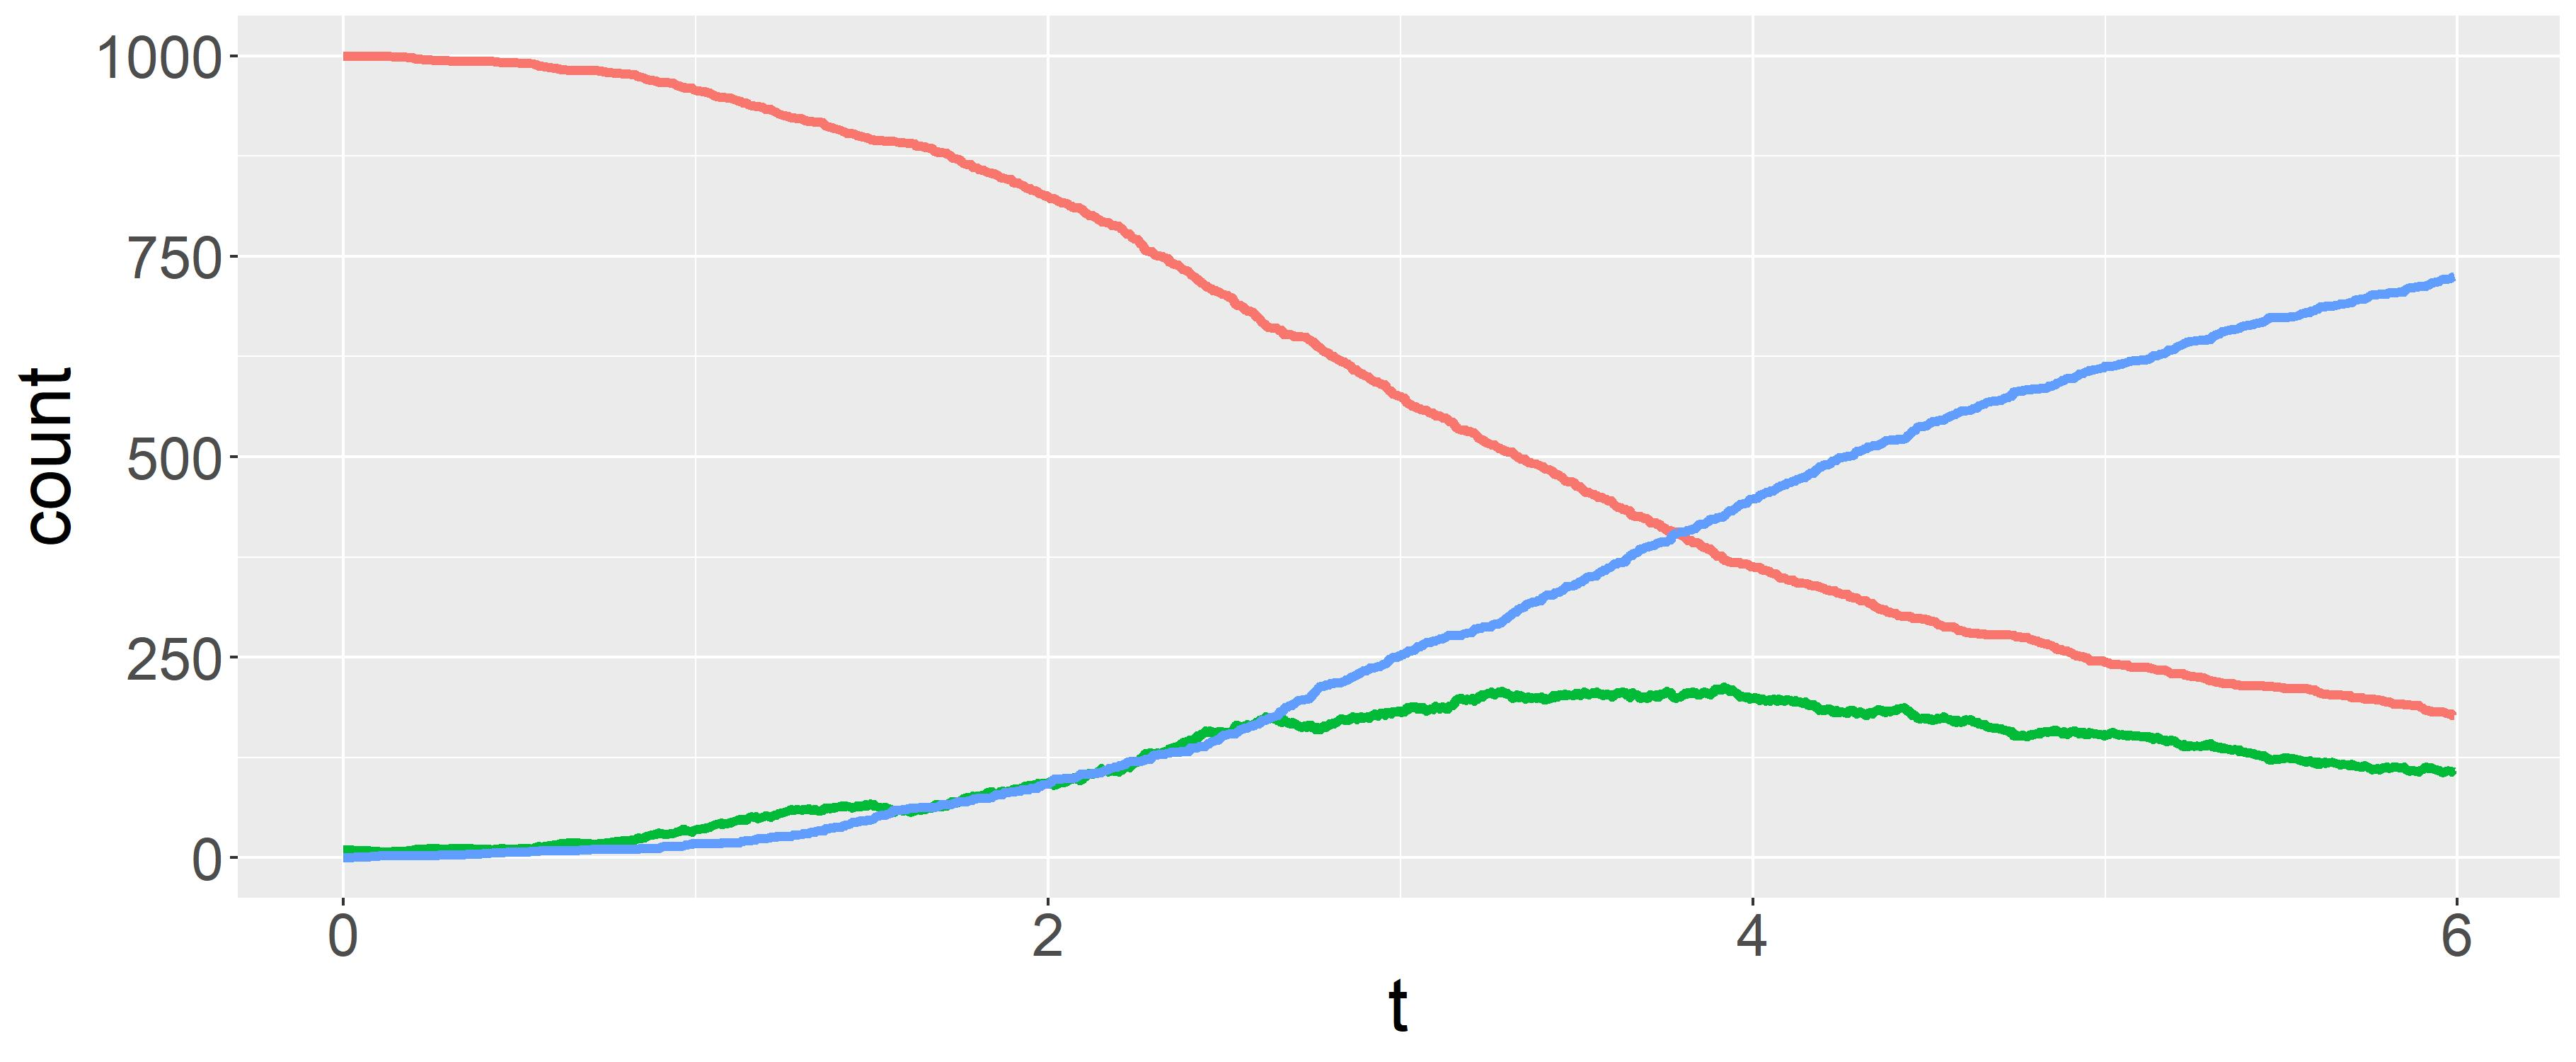
\includegraphics[width=\textwidth]{E1_trajectories}
			\caption{Compartment trajectories}
			\label{fig:E1_trajectories}
		\end{subfigure}
		\hfill
		\begin{subfigure}[b]{0.41\textwidth}
			\centering
			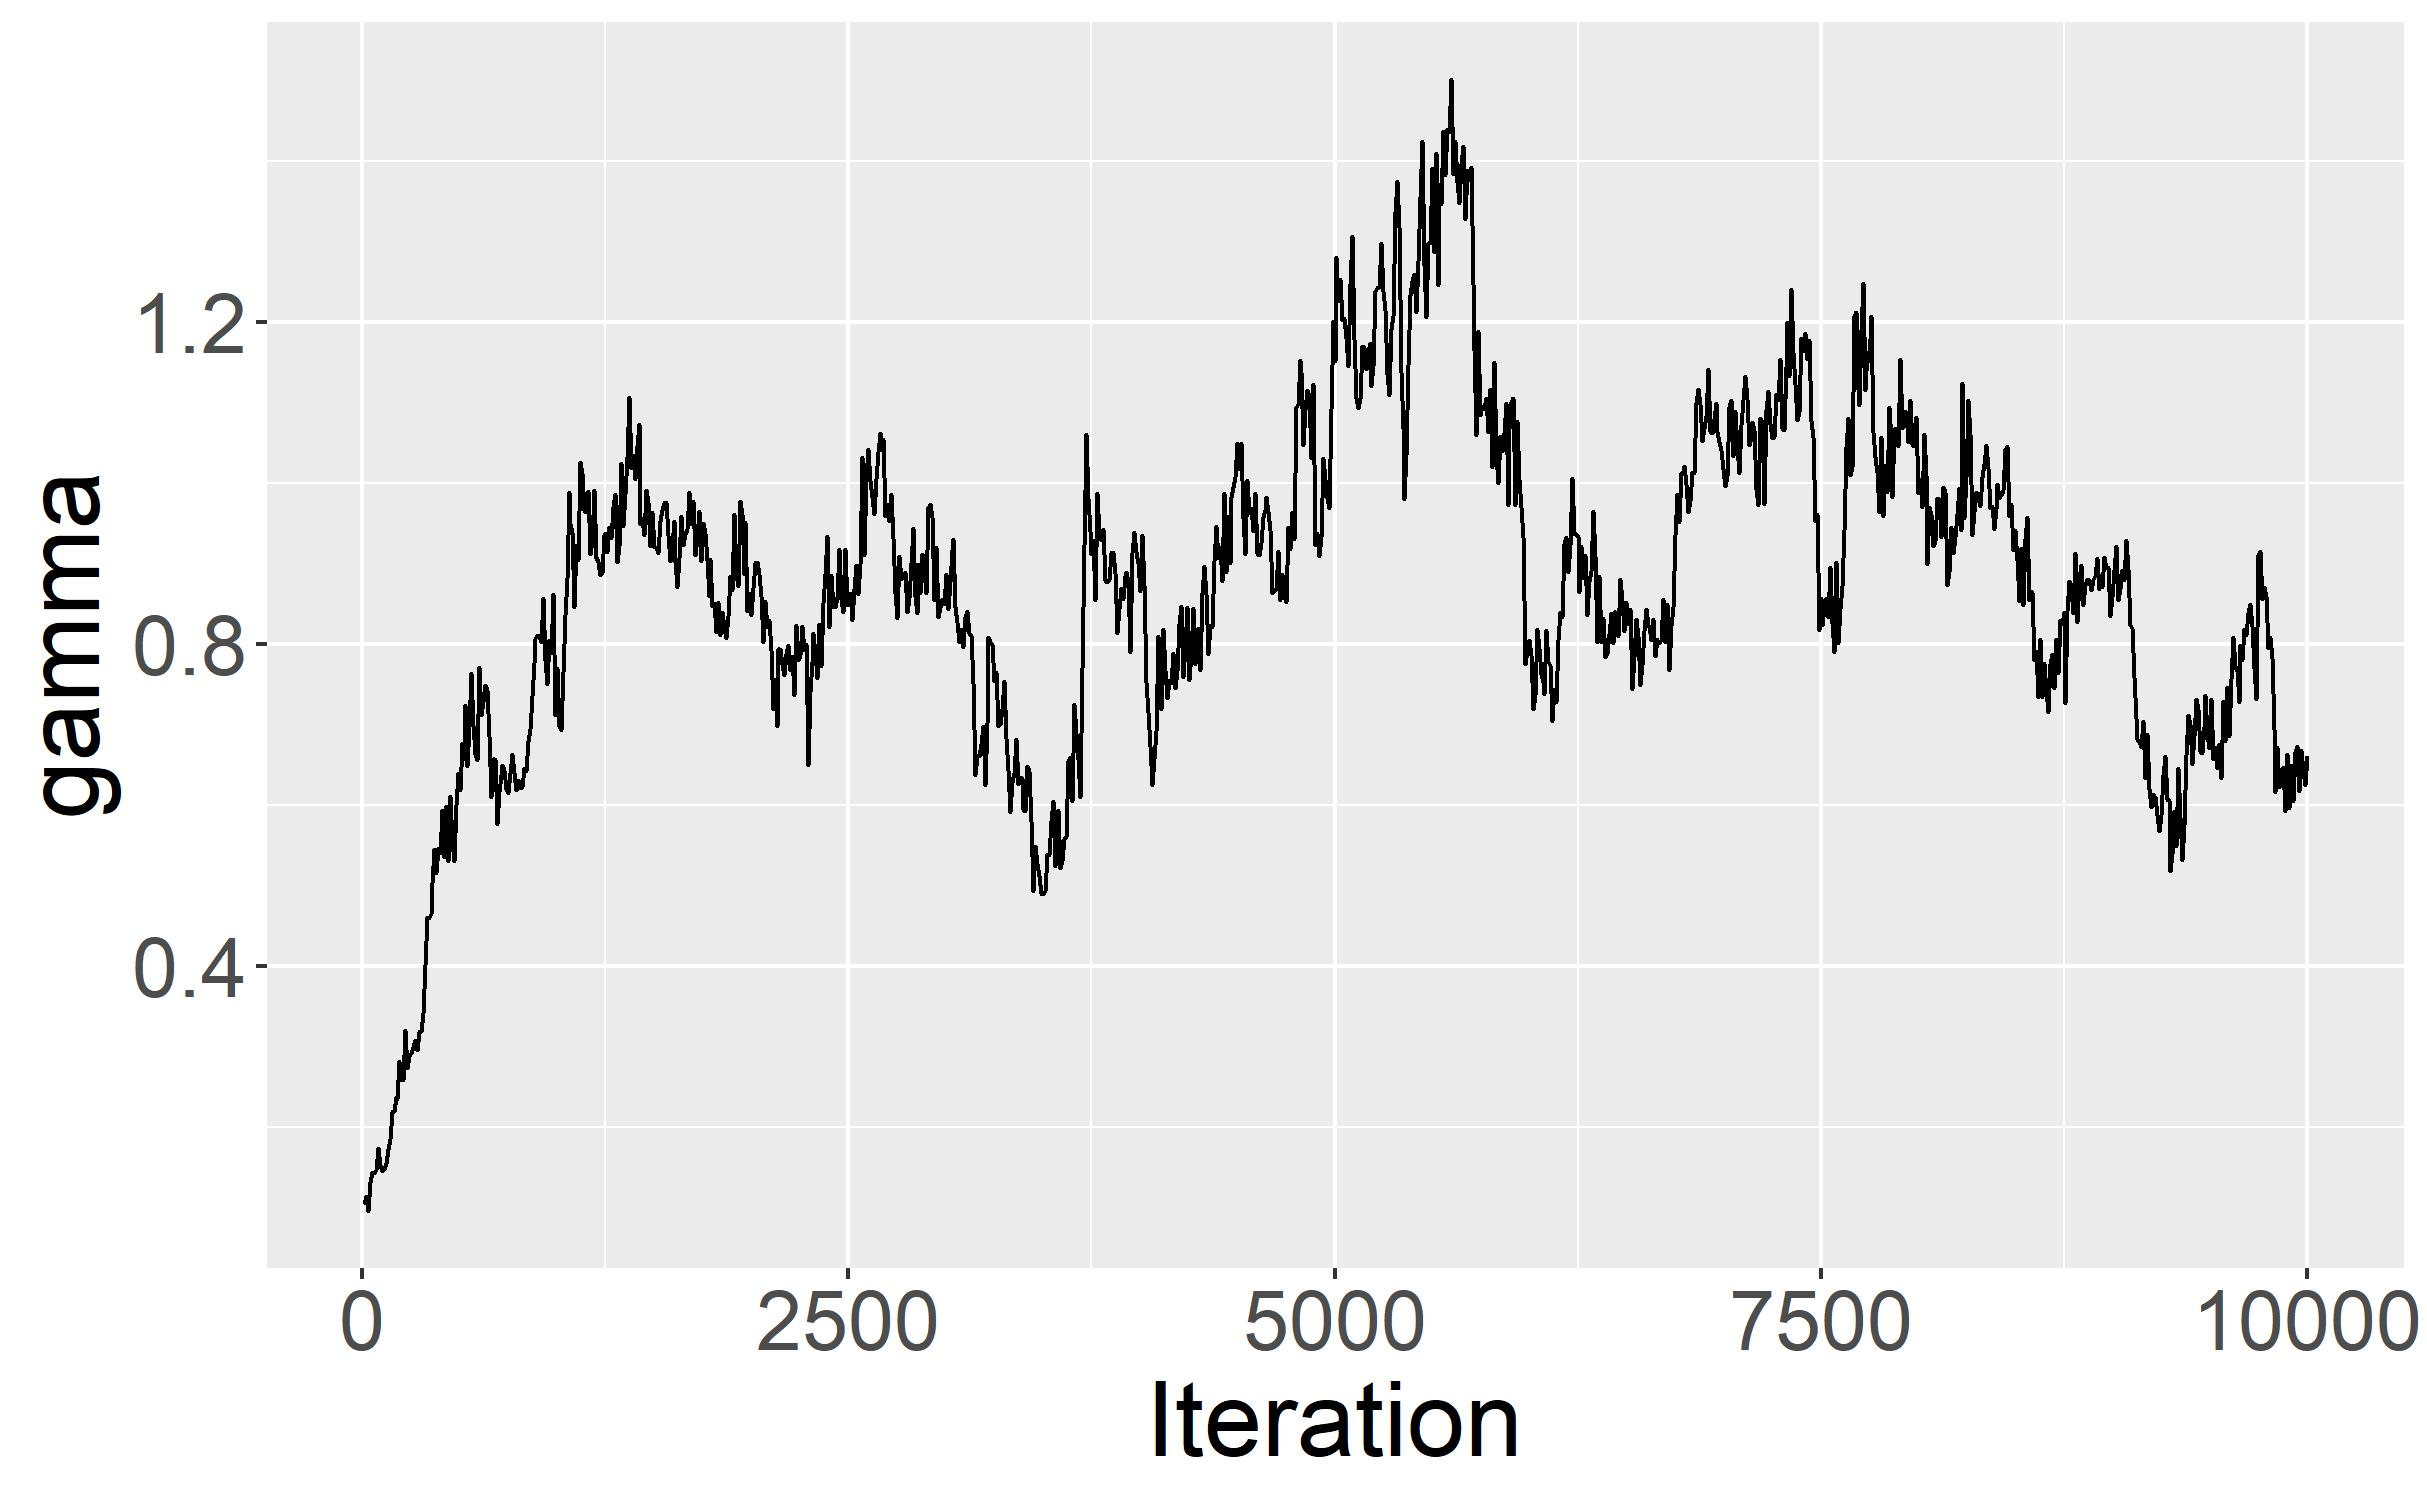
\includegraphics[width=\textwidth]{E1_short_no_burn_gamma_tp}
			\caption{Traceplot of $\gamma$ during the transient phase}
			\label{fig:E1_short_no_burn_gamma_tp}
		\end{subfigure}
		\\
		\begin{subfigure}[b]{0.41\textwidth}
			\centering
			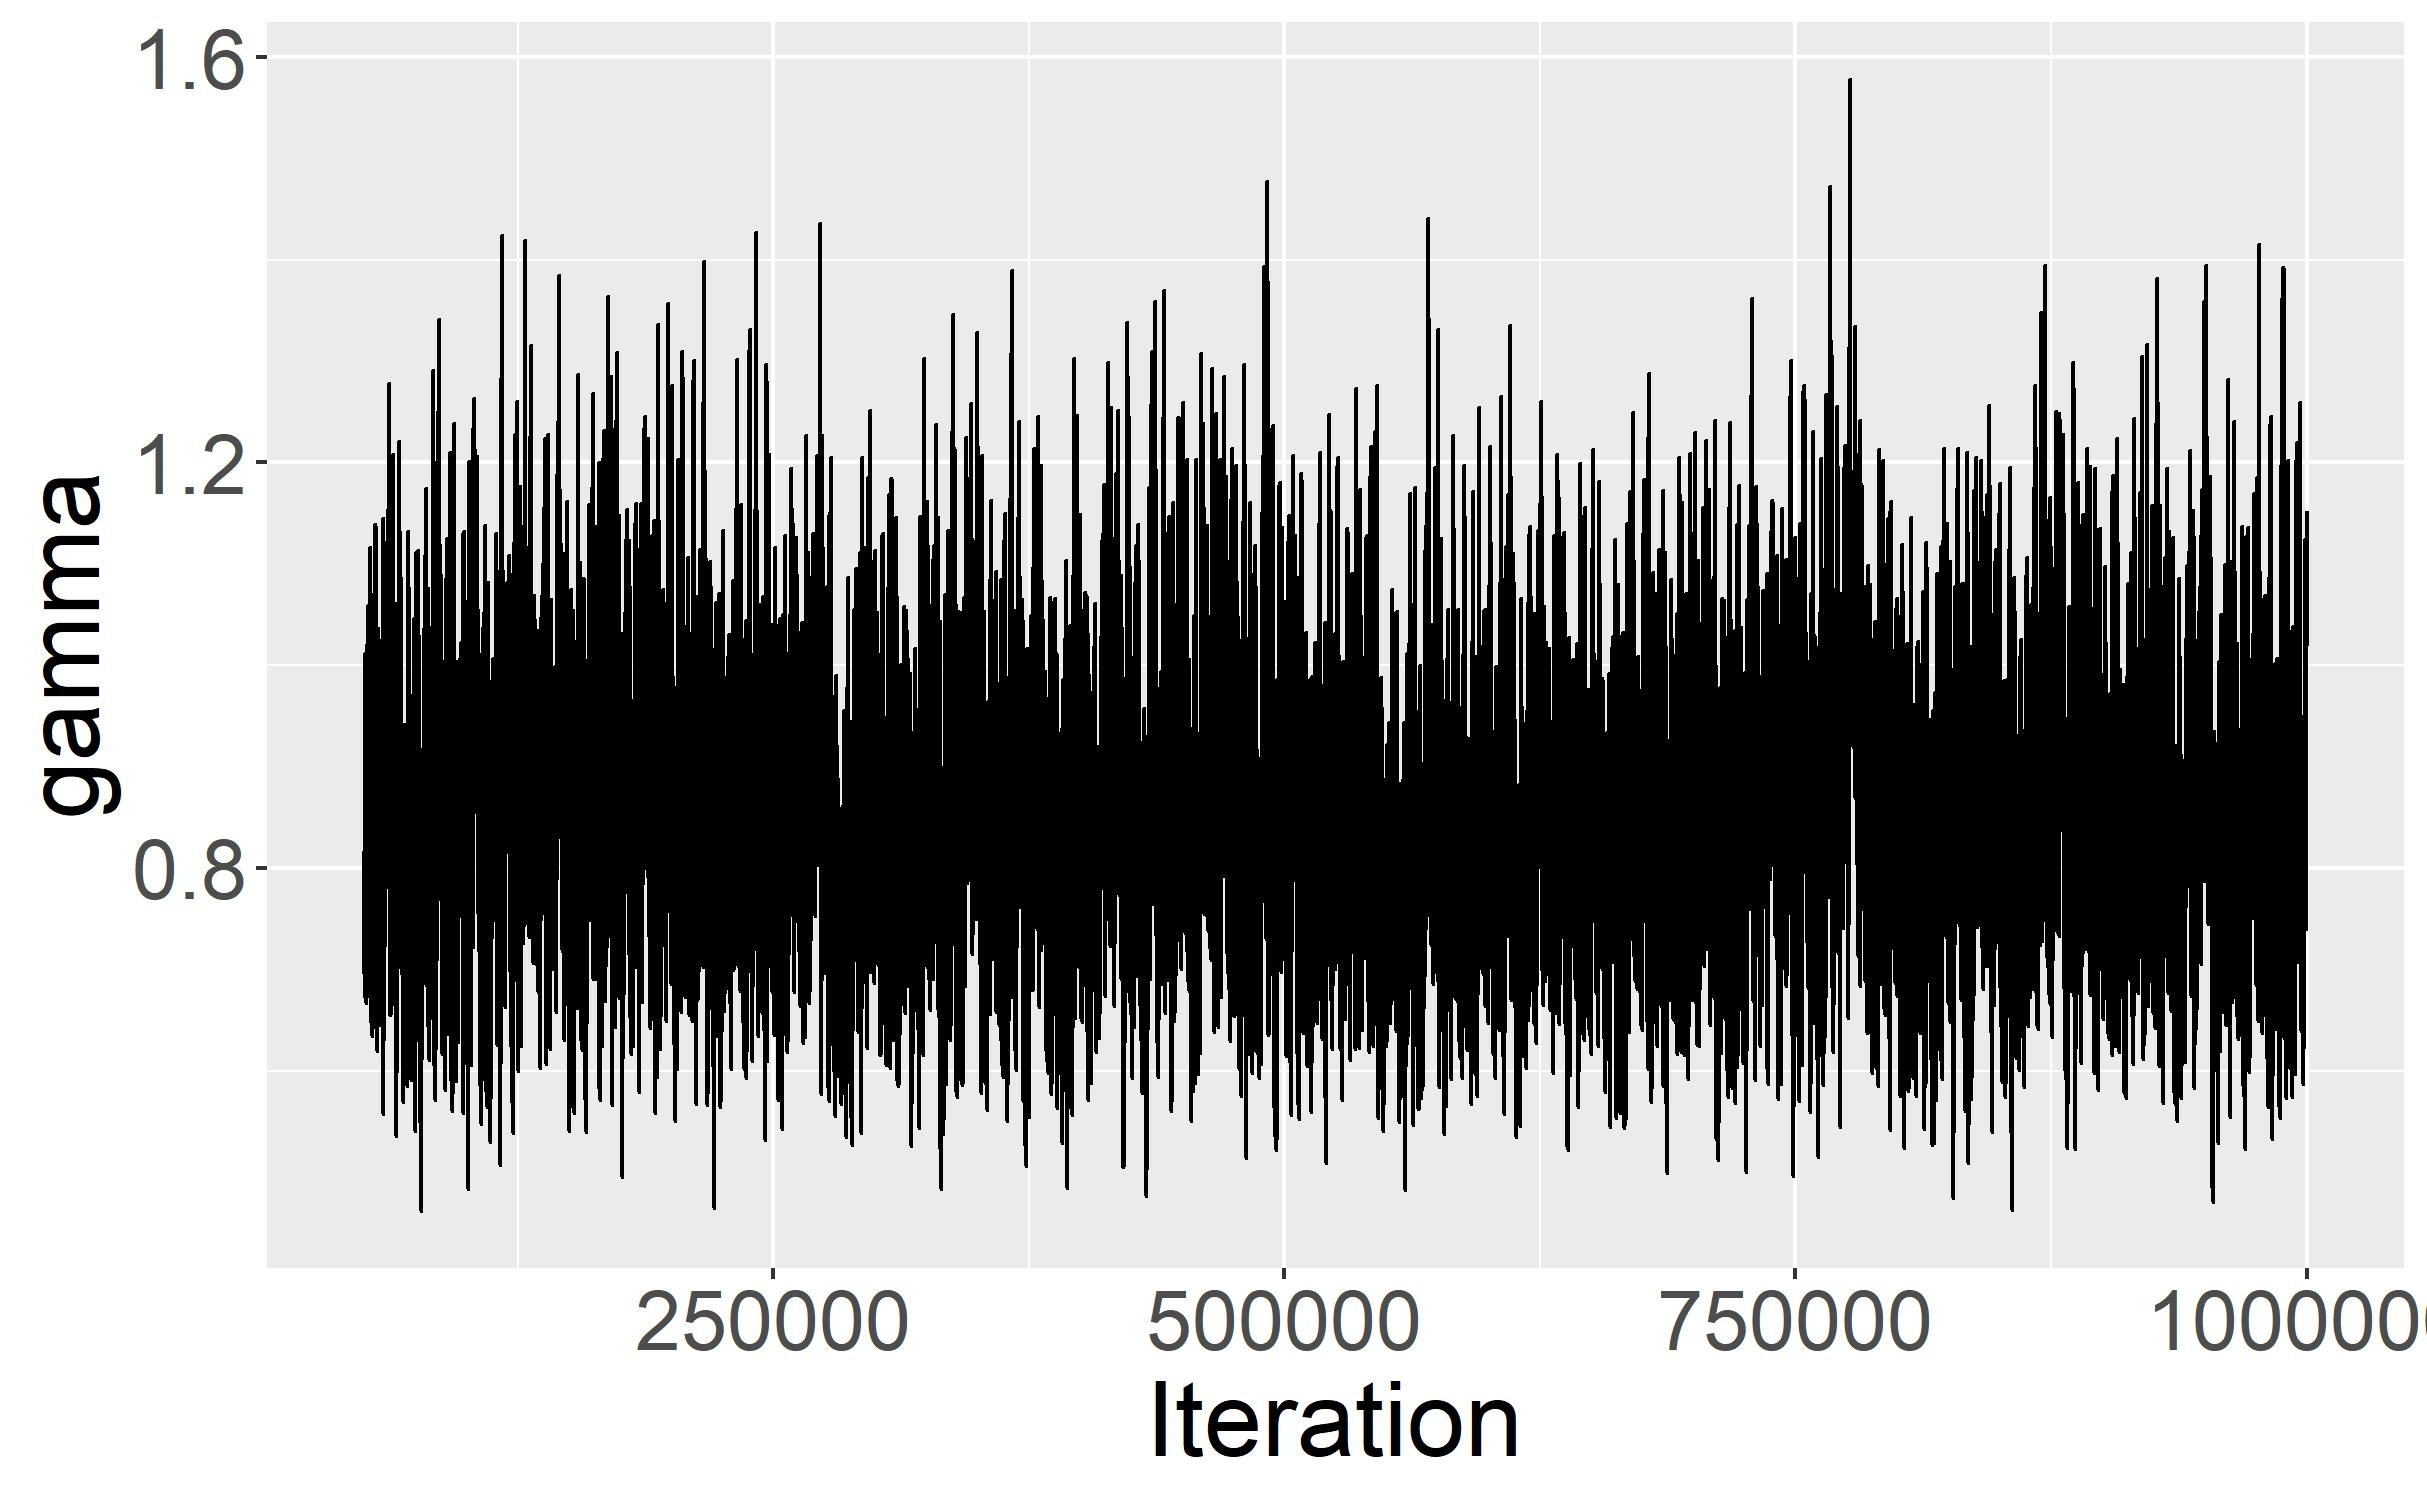
\includegraphics[width=\textwidth]{E1_burn_gamma_tp}
			\caption{Traceplot of $\gamma$ after the transient phase}
			\label{fig:E1_burn_gamma_tp}
		\end{subfigure}
		\hfill
		\begin{subfigure}[b]{0.41\textwidth}
			\centering
			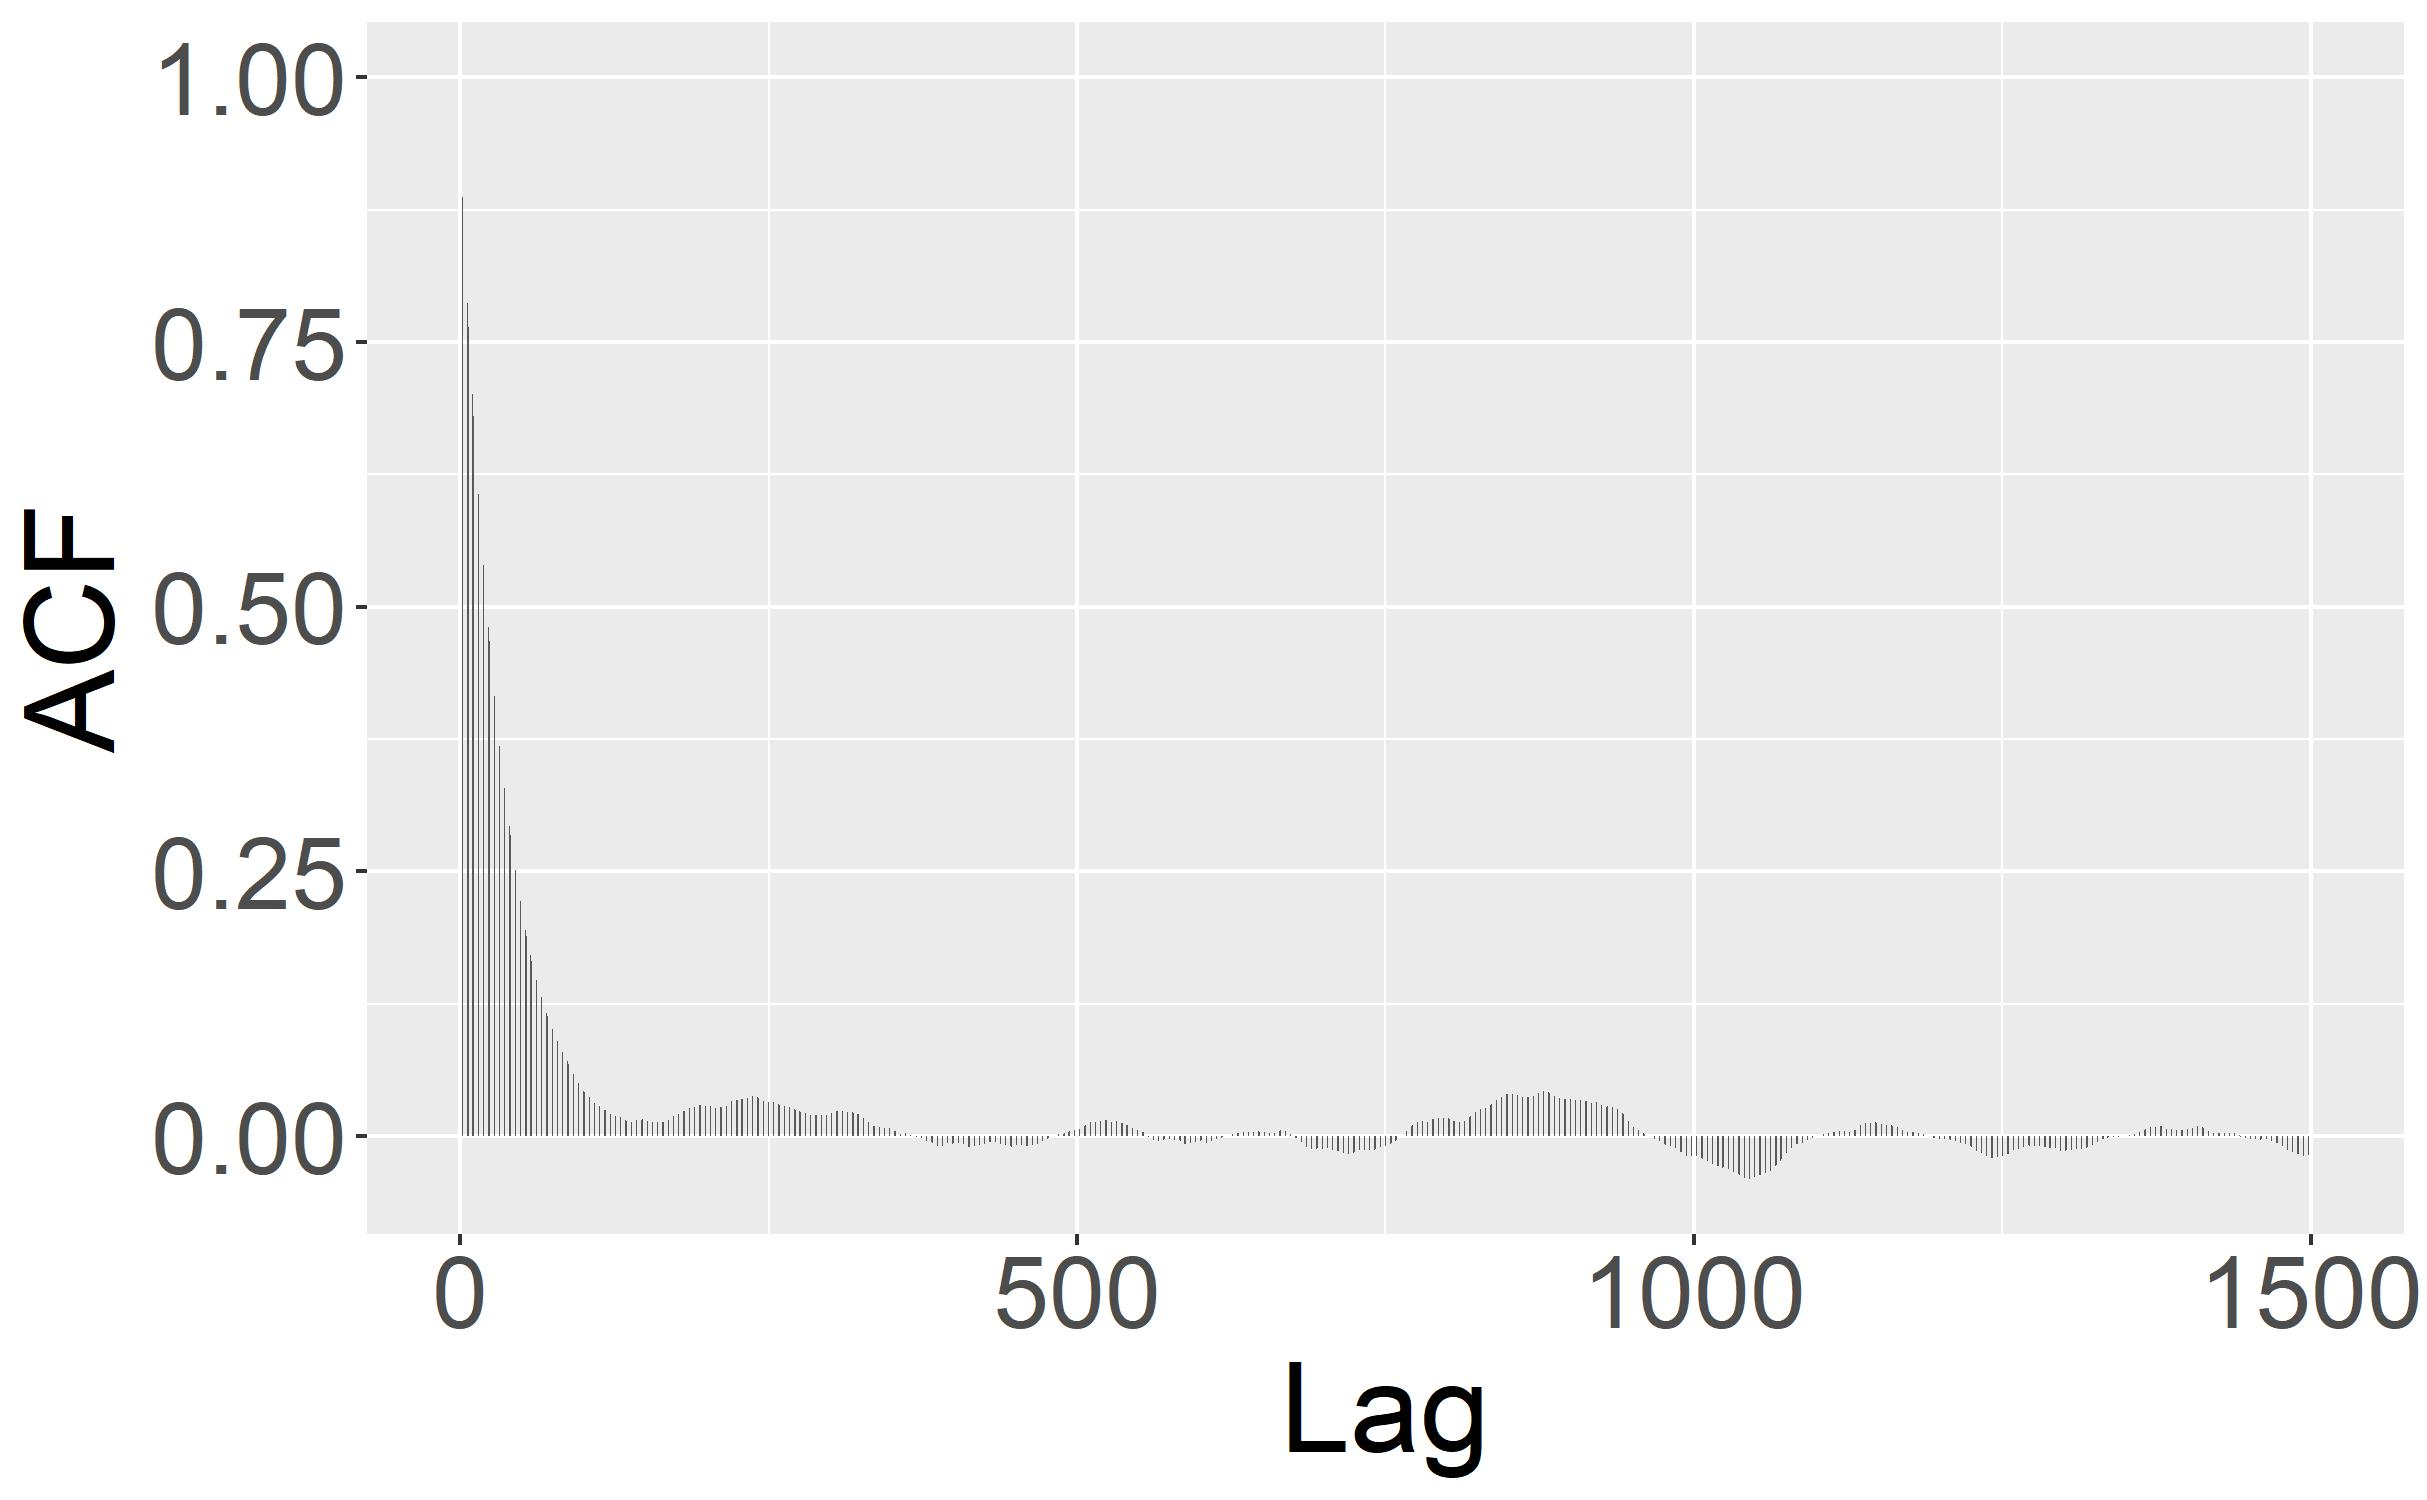
\includegraphics[width=\textwidth]{E1_burn_gamma_acf}
			\caption{Auto-correlation function for $\gamma$}
			\label{fig:E1_burn_gamma_acf}
		\end{subfigure}
		\caption{Performance of the proposed DA-MCMC in a medium-sized population $(S(0), I(0)) = (1000, 10)$ for the parameter $\gamma$.}
		\label{fig:E1}
	\end{figure}
	
    \begin{table}
    \centering
    \begin{tabular}{ |C{2cm}| *{3}{C{3cm}}|}
        \hline
        Parameter & Coverage rate of the $90\%$ credible intervals & Average of the posterior means & SD of the posterior means \\ 
        \hline
        $\beta$ & 0.895 & 0.0025 & 0.000255\\ 
        $\gamma$ & 0.902 & 1.00 & 0.142 \\ 
        $R_0$ & 0.910 & 2.54 & 0.194 \\
        \hline
    \end{tabular}
    \caption{Empirical coverage of  $90\%$ posterior credible intervals and distribution of the posterior means from $2000$ independent runs in a medium-sized population. The true values of the parameters are $(\beta. \gamma. R_0) = (0.0025, 1, 2.5)$.}
    \label{tab:coverage}
    \end{table}
	
	Second, we explore the impact of the tuning parameter $\rho$ on the mixing properties of the algorithm across different population sizes.
	We simulate three SIR processes with $S(0) \in \{250, 500, 1000\}$. We set $I(0)=10$, $\gamma=1$, $t_{end} = 6$ and $K = 10$ for each simulation and use $R_0 \in \{3, 2.5, 2\}$ respectively for the different population sizes. These values for $R_0$ were chosen to give pandemics with comparable dynamics. We consider the values $\rho \in \{0.02, 0.05, 0.1, 0.25, 0.5, 1\}$. For each population size and each value of $\rho$, the DA-MCMC algorithm is run for $1$ million iterations. %Note that the algorithm is not run if the number of trajectories updated $\rho(S_0+I_0)$ is smaller than $1$.
	
	Figure \ref{fig:E3_runtime} and \ref{fig:E3_accept} present the run time of the algorithm and the acceptance rate in the Metropolis-Hastings step. We observe that the run time increases with the population size and with $\rho$ and that, as expected, the acceptance rate decreases as the number of trajectories updated per iteration $\rho(S(0)+I(0))$ increases.
	Finally, Figure \ref{fig:E3_facet_ESSsecR0} shows the effect of $\rho$ on the auto correlation function for the parameter $\beta$ for the medium-size population process ($S(0) = 1,000$) for three values of $\rho$. We observe that updating half of the augmented data per iteration yields the lowest auto-correlation function across the values of $\rho$ considered. This suggests that, in this setting, updating the entire latent space in the Metropolis-Hastings step results in too many rejections, while updating a tenth or less prevents the chain from efficiently exploring the latent space.
	
	
	\begin{figure}
		\centering
		\begin{subfigure}[b]{0.42\textwidth}
			\centering
			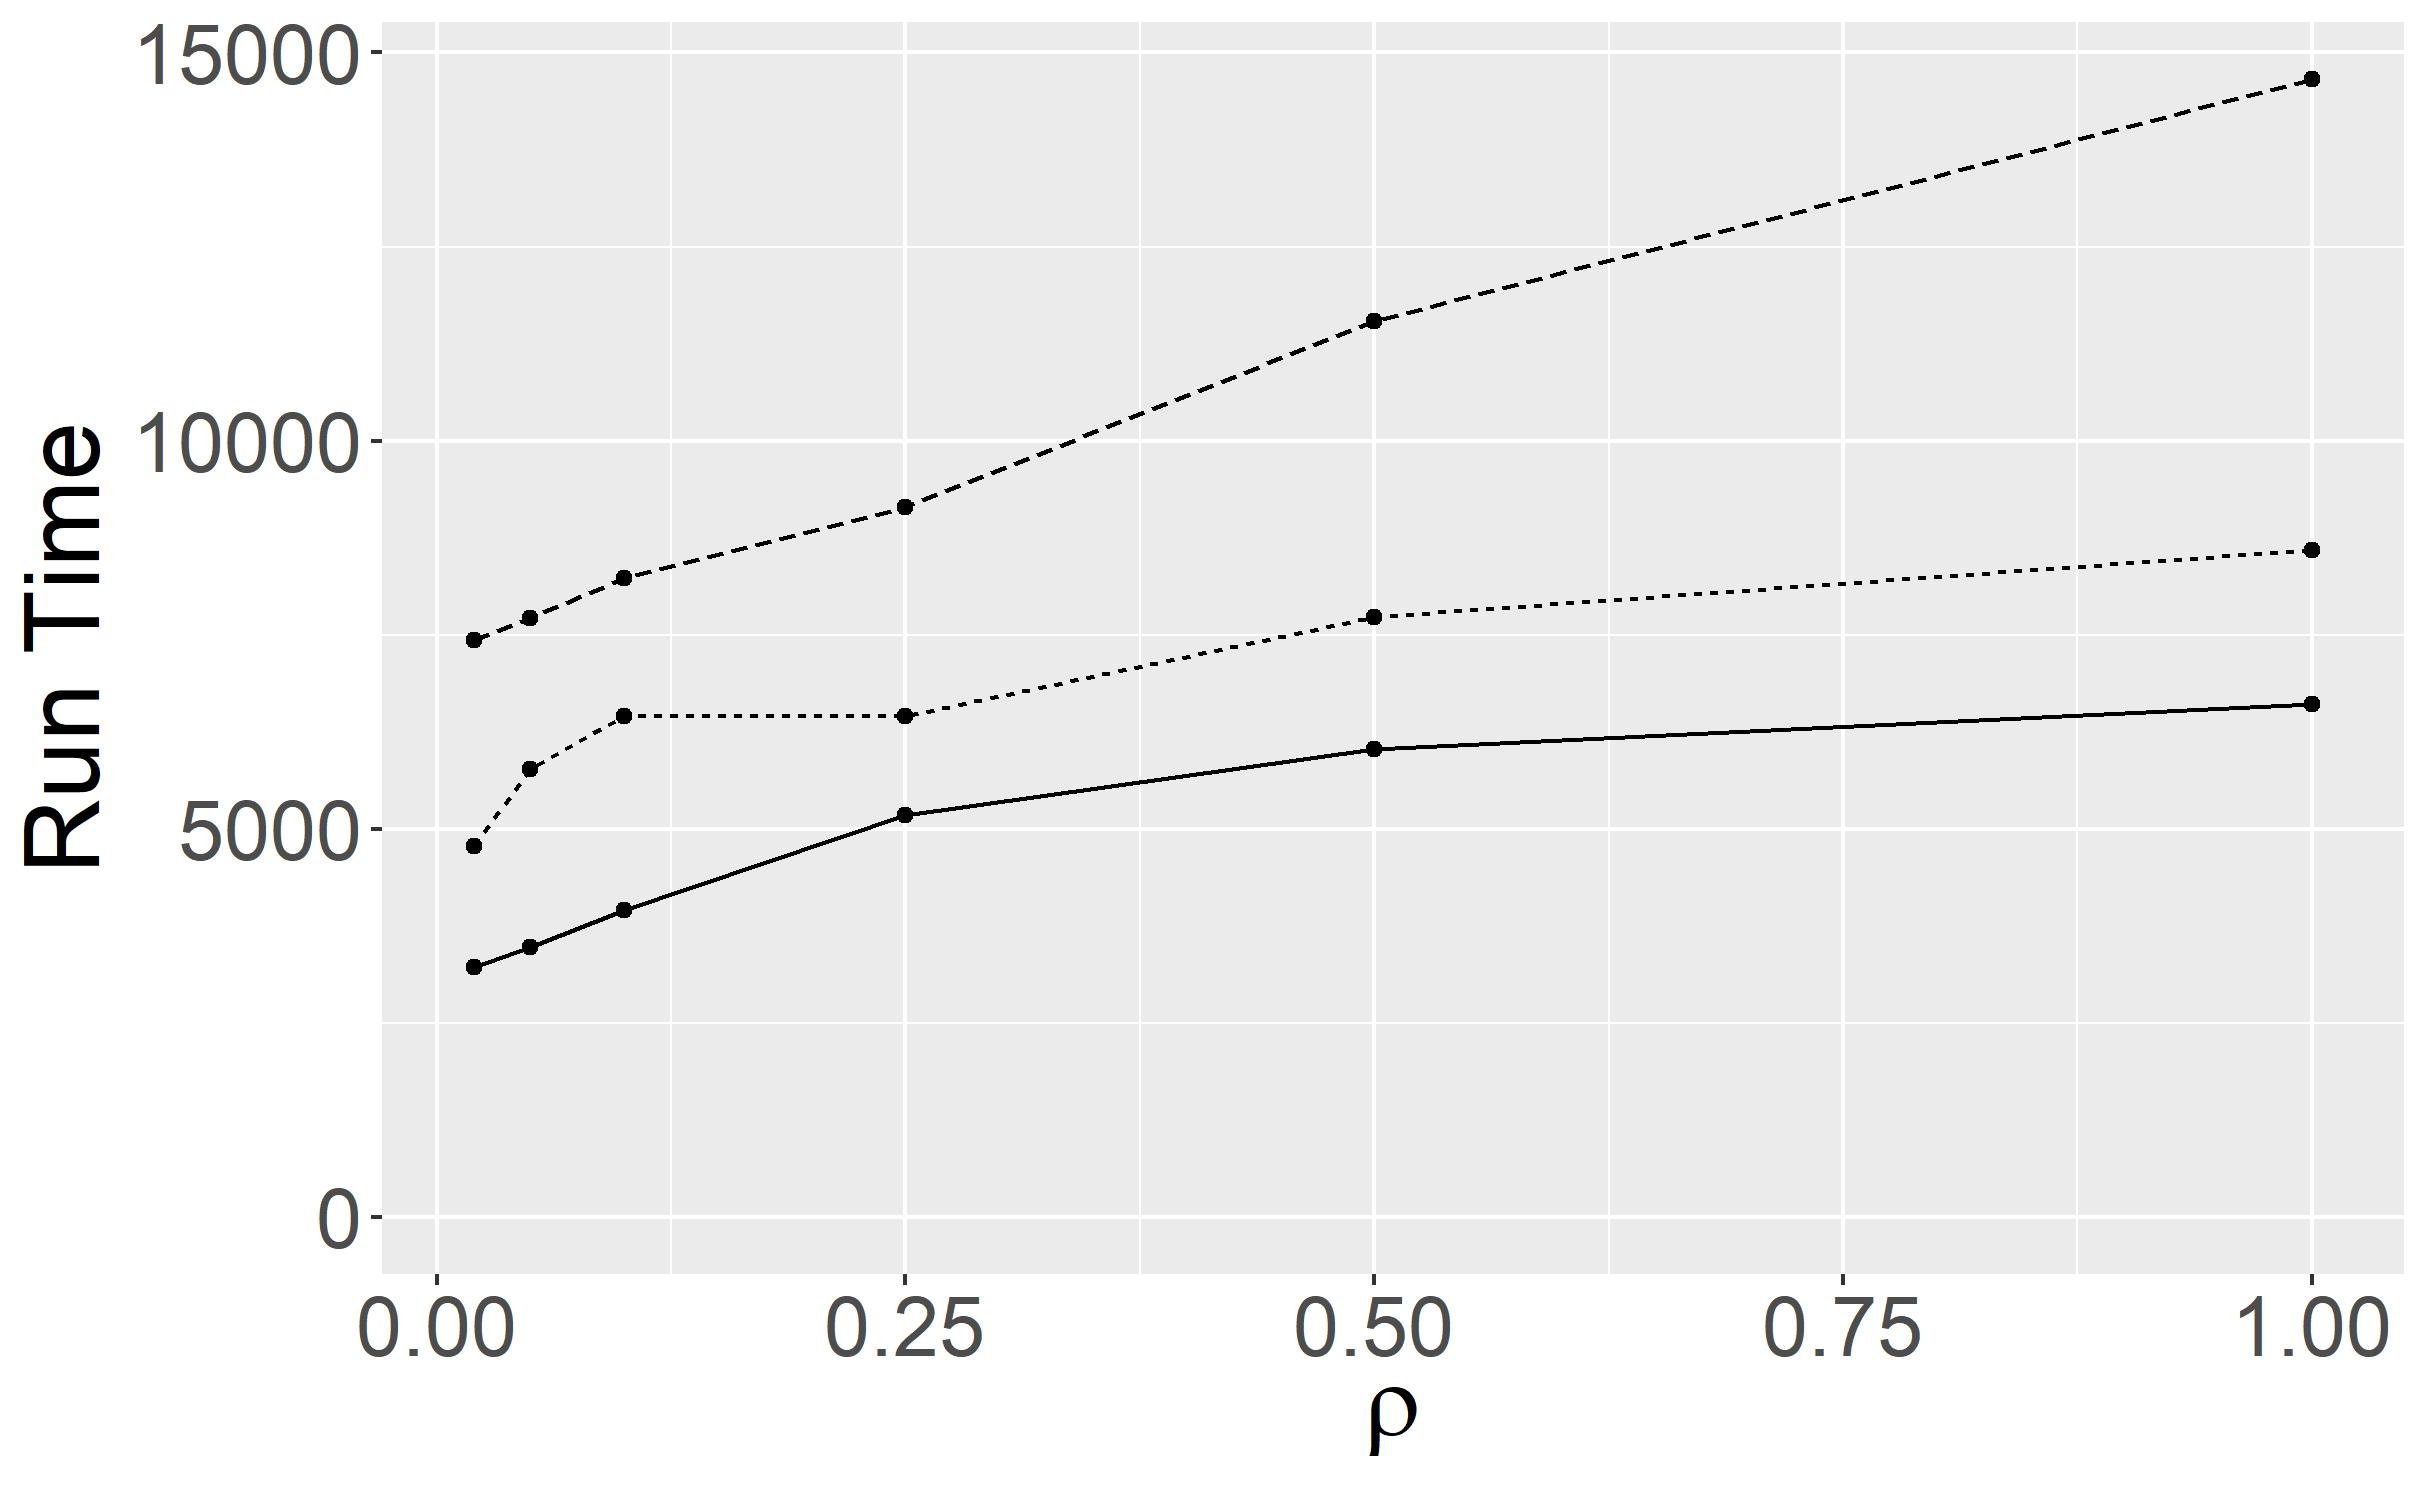
\includegraphics[width=\textwidth]{E3_runtime}
			\caption{Run time in minutes}
			\label{fig:E3_runtime}
		\end{subfigure}
		\hfill
		\begin{subfigure}[b]{0.41\textwidth}
			\centering
			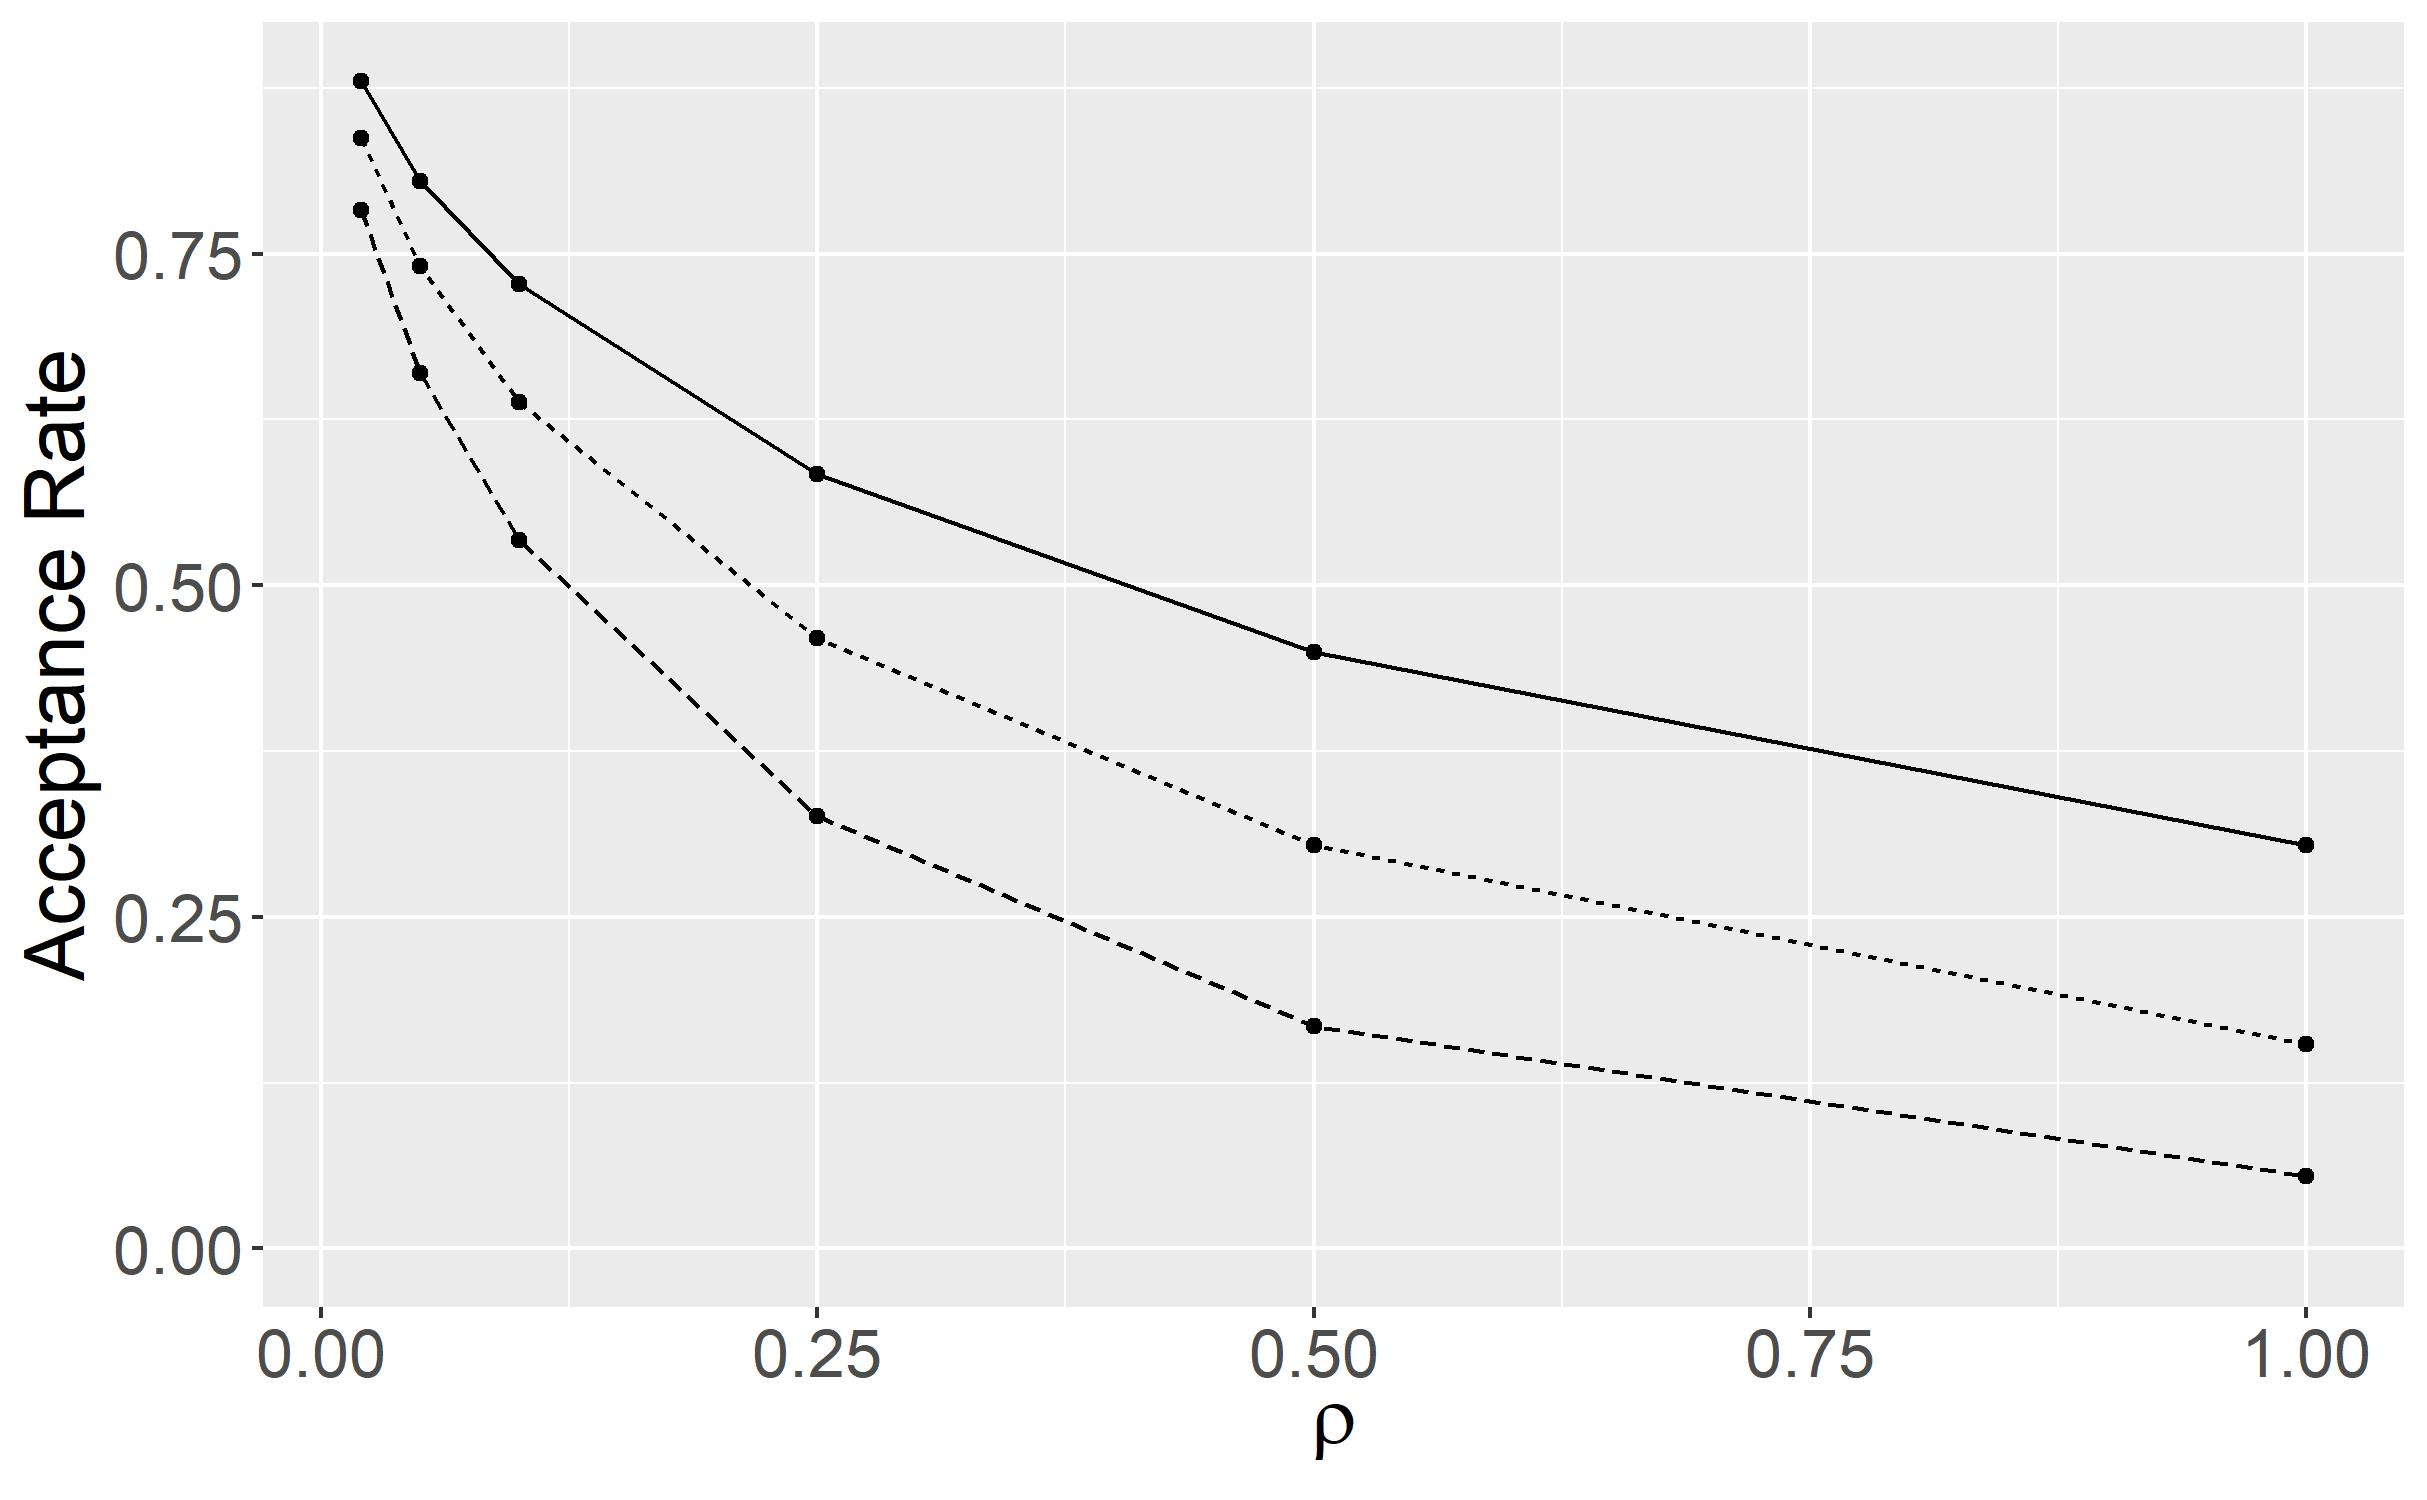
\includegraphics[width=\textwidth]{E3_accept}
			\caption{Acceptance rate}
			\label{fig:E3_accept}
		\end{subfigure}
		\\
		\begin{subfigure}[b]{0.41\textwidth}
			\centering
			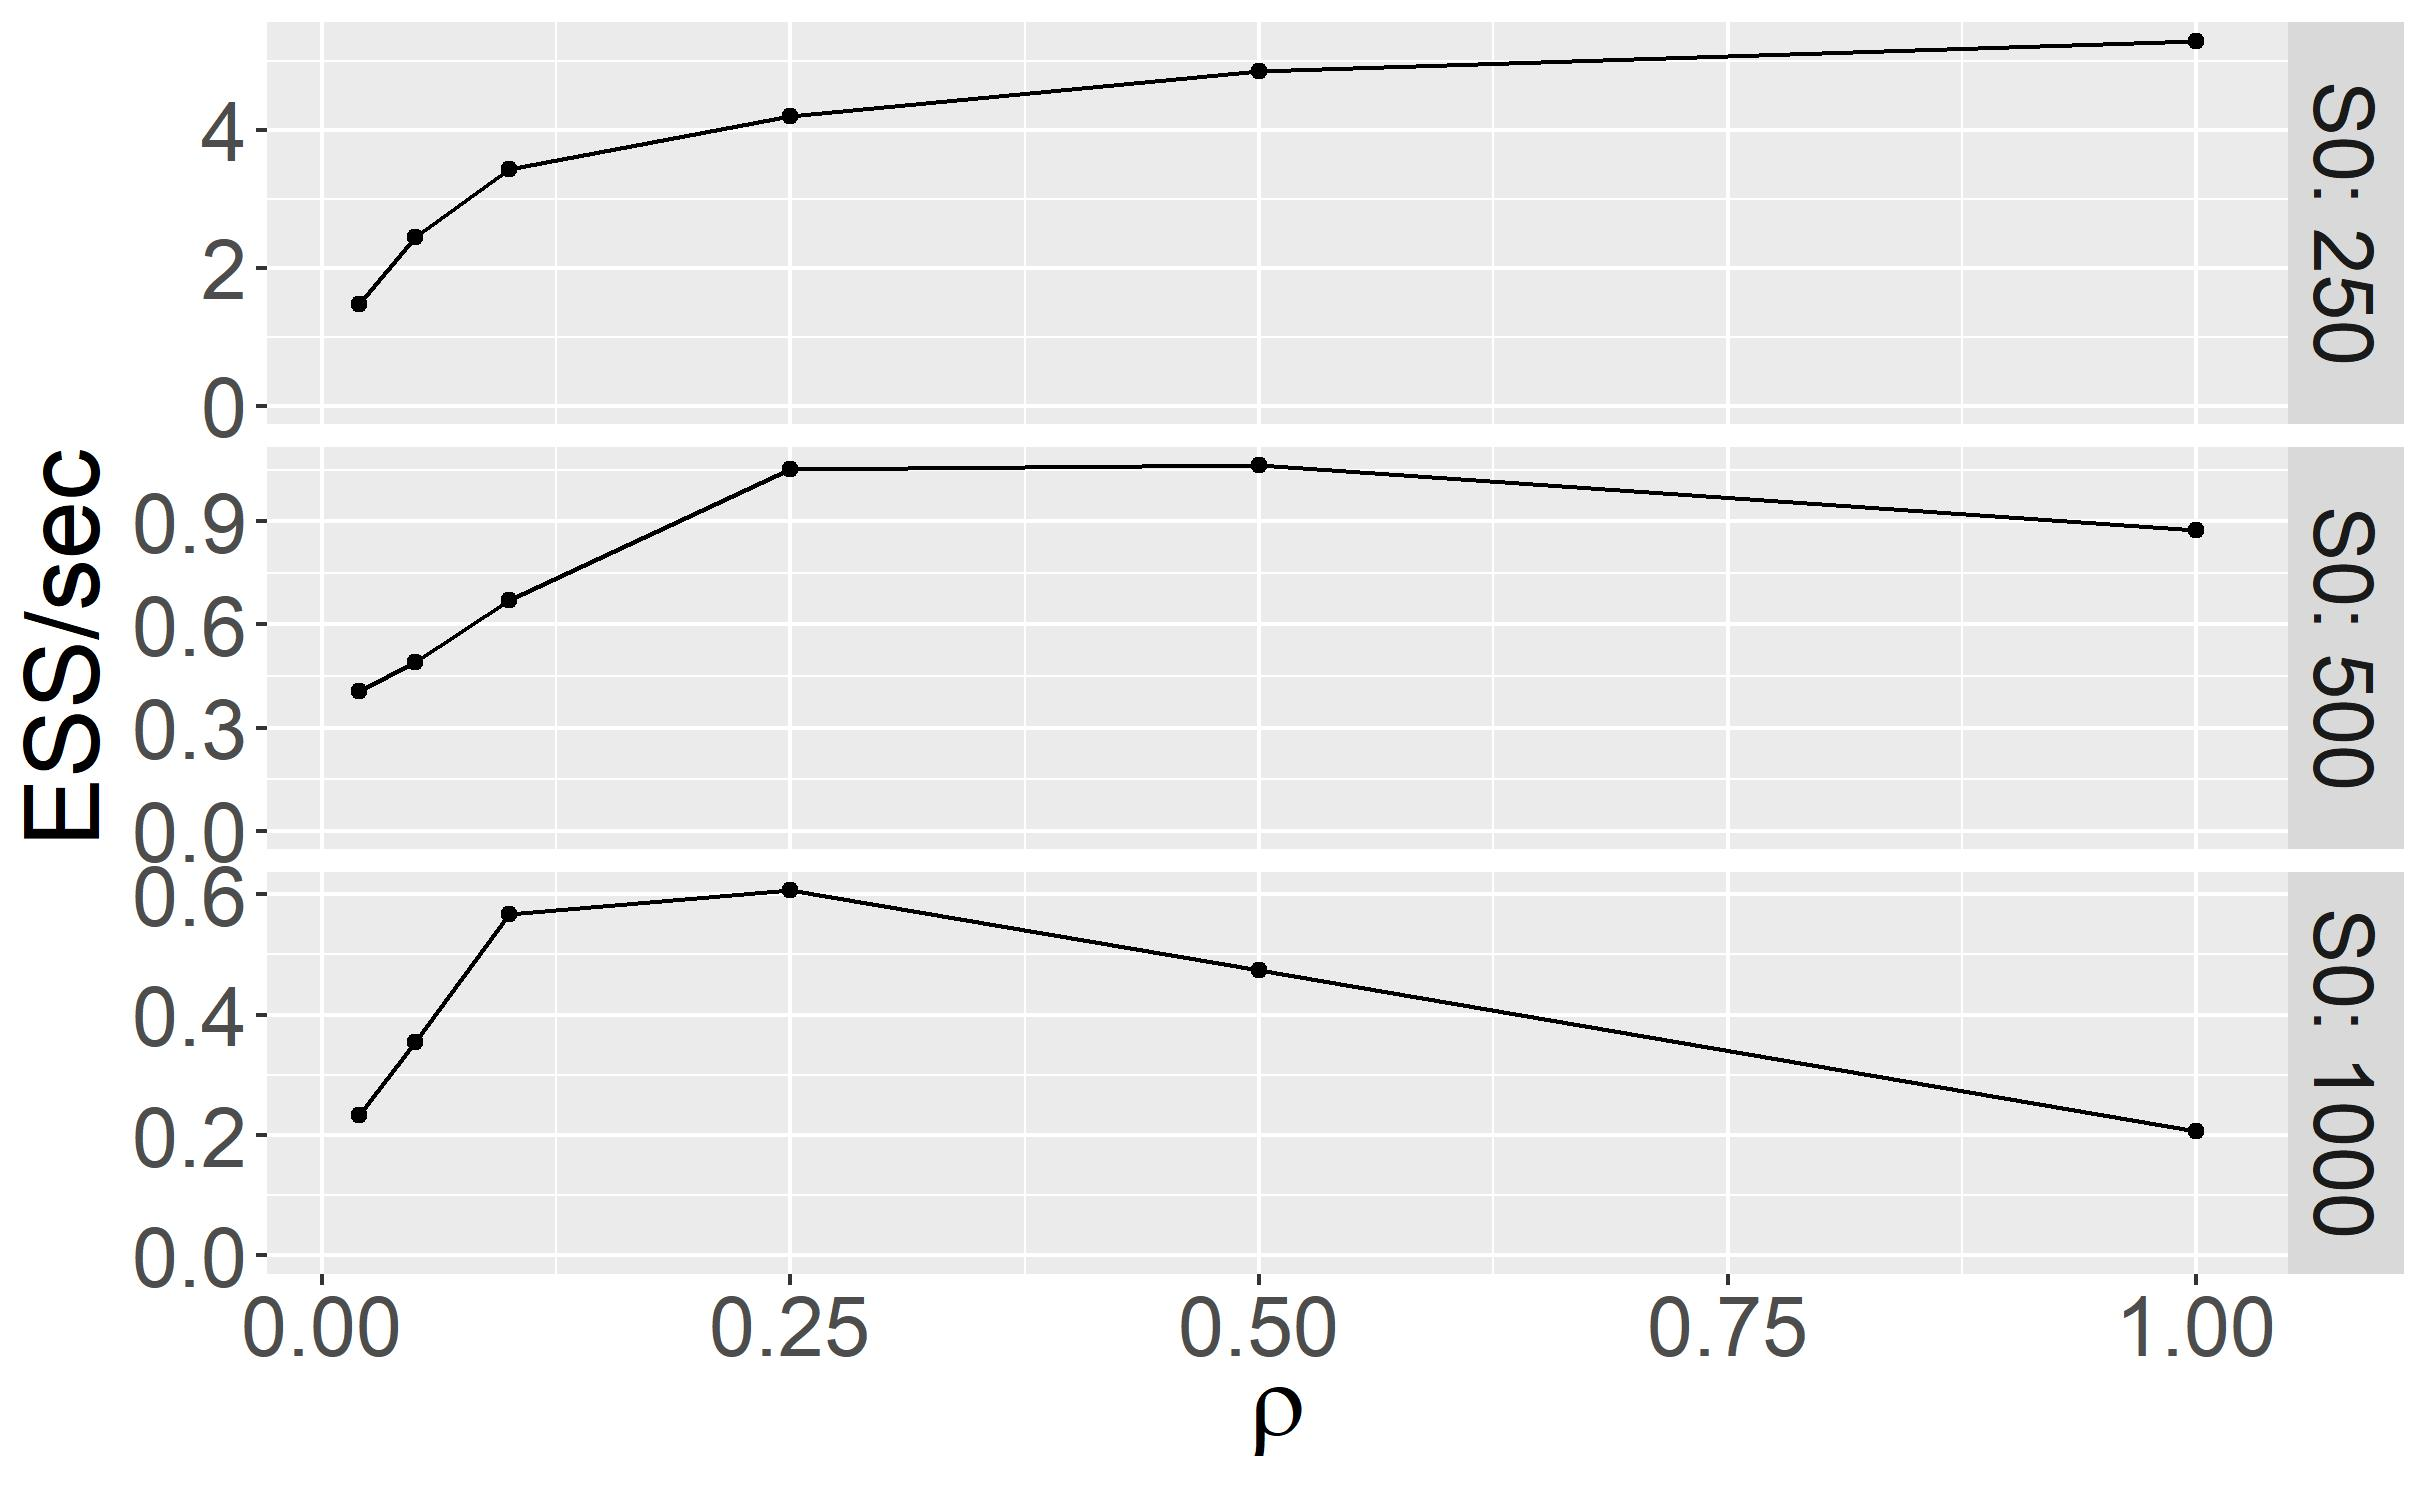
\includegraphics[width=\textwidth]{E3_facet_ESSsecR0}
			\caption{ESS/sec for $R_0$
			%Acceptance rate of the proposed latent spaces in the Metropolis-Hastings step of the MCMC algorithm across different population sizes and values for $\rho$.
			}
			\label{fig:E3_facet_ESSsecR0}
		\end{subfigure}
		\caption{Impact of $\rho$ on the performance of the DA-MCMC across different population sizes.}
		\label{fig:E3}
	\end{figure}
		
	Finally, we compare the performance of the proposed DA-MCMC algorithm in which event times are jointly proposed to that of a single-site-update DA-MCMC (SSU DA-MCMC) that is similar in spirit to \cite{Gibson.1998, ONeill.1999, Fintzi.2017}. The SSU DA-MCMC that we consider here is a special case of the proposed DA-MCMC in which $\rho = (S(0)+I(0))^{-1}$, so that the infection and removal times of a single individual are updated per iteration. The two algorithms are run on the same data for $1$ million iterations. Figure \ref{fig:E6} presents the traceplots for $\gamma$ as well as the auto-correlation function. We observe that the Markov chain mixes much better when event times are jointly proposed in the Metropolis-Hastings step. This is supported quantitatively in Table \ref{tab:E6} which shows that the effective sample size per second obtained with the proposed DA-MCMC is between 7 and 20 times larger than that of the SSU DA-MCMC.
	
	
 \ram{explain why not compare chain binomial, particle filtering (forward simulation), LNA requires noisy data.}
	
	\begin{figure}
		\centering
		\begin{subfigure}[b]{0.42\textwidth}
			\centering
			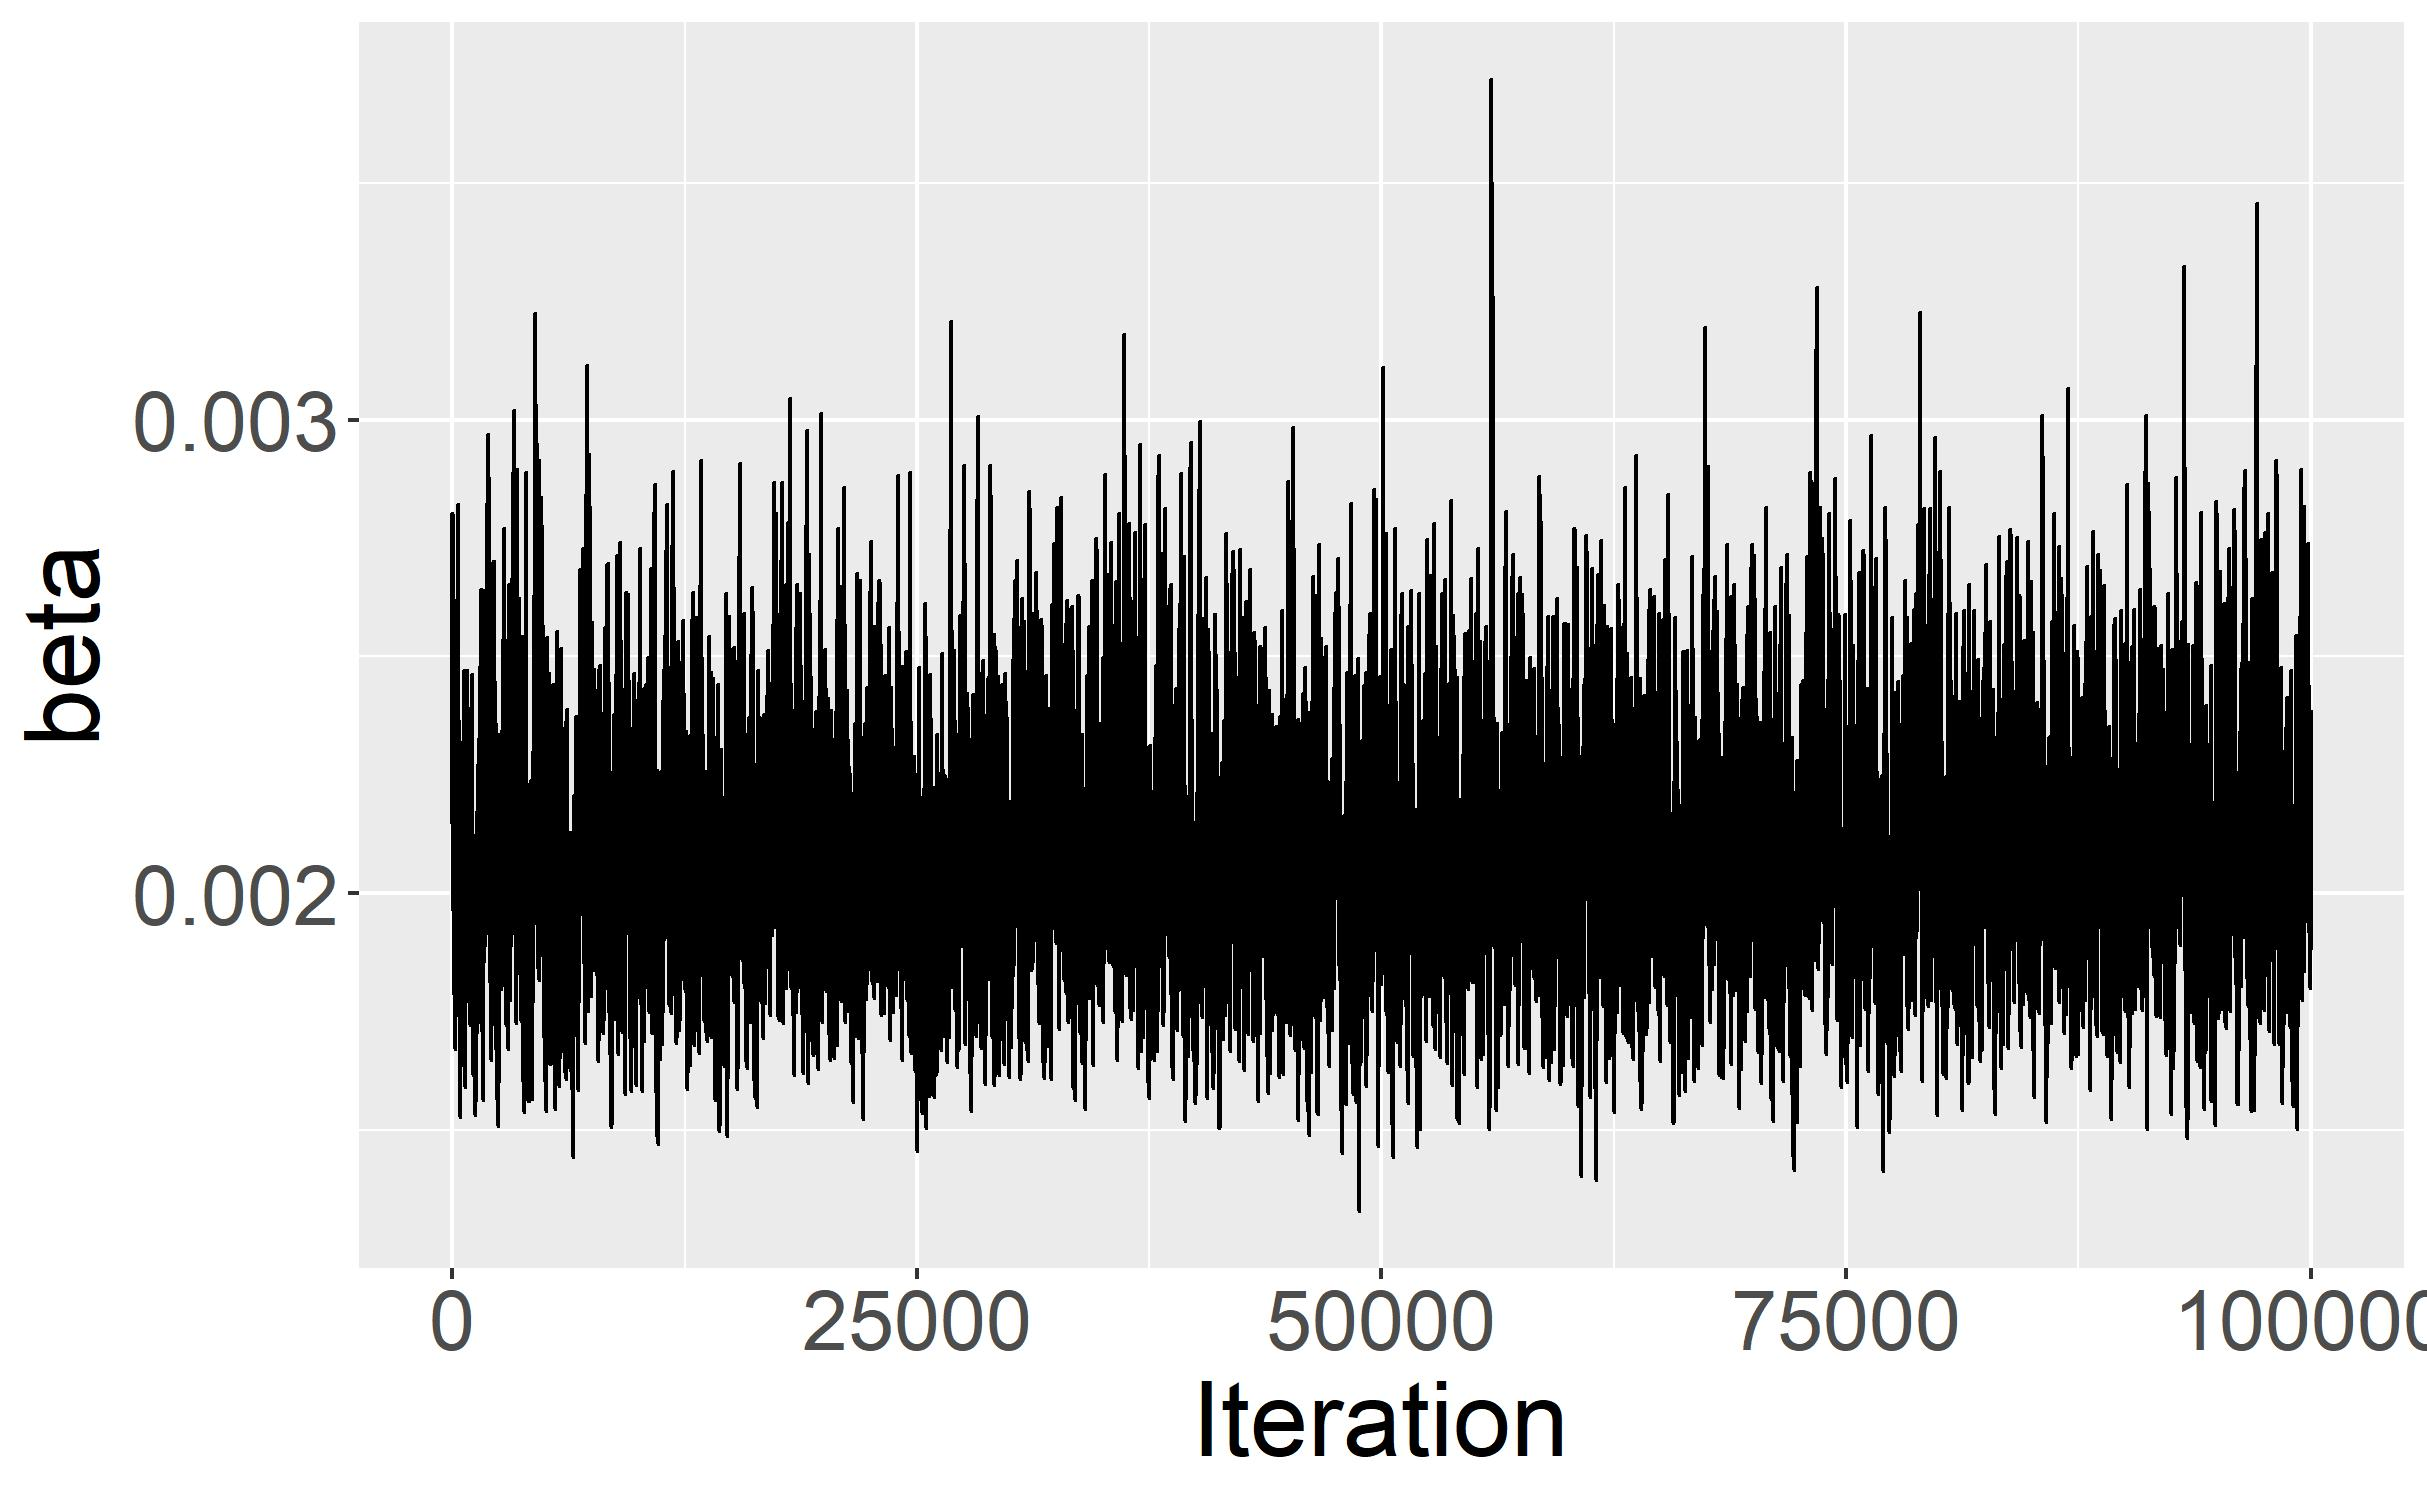
\includegraphics[width=\textwidth]{E6_no_burn_beta_tp_joint.jpg}
			\caption{DA-MCMC}
			\label{fig:E6_no_burn_beta_tp_joint}
		\end{subfigure}
		\hfill
		\begin{subfigure}[b]{0.41\textwidth}
			\centering
			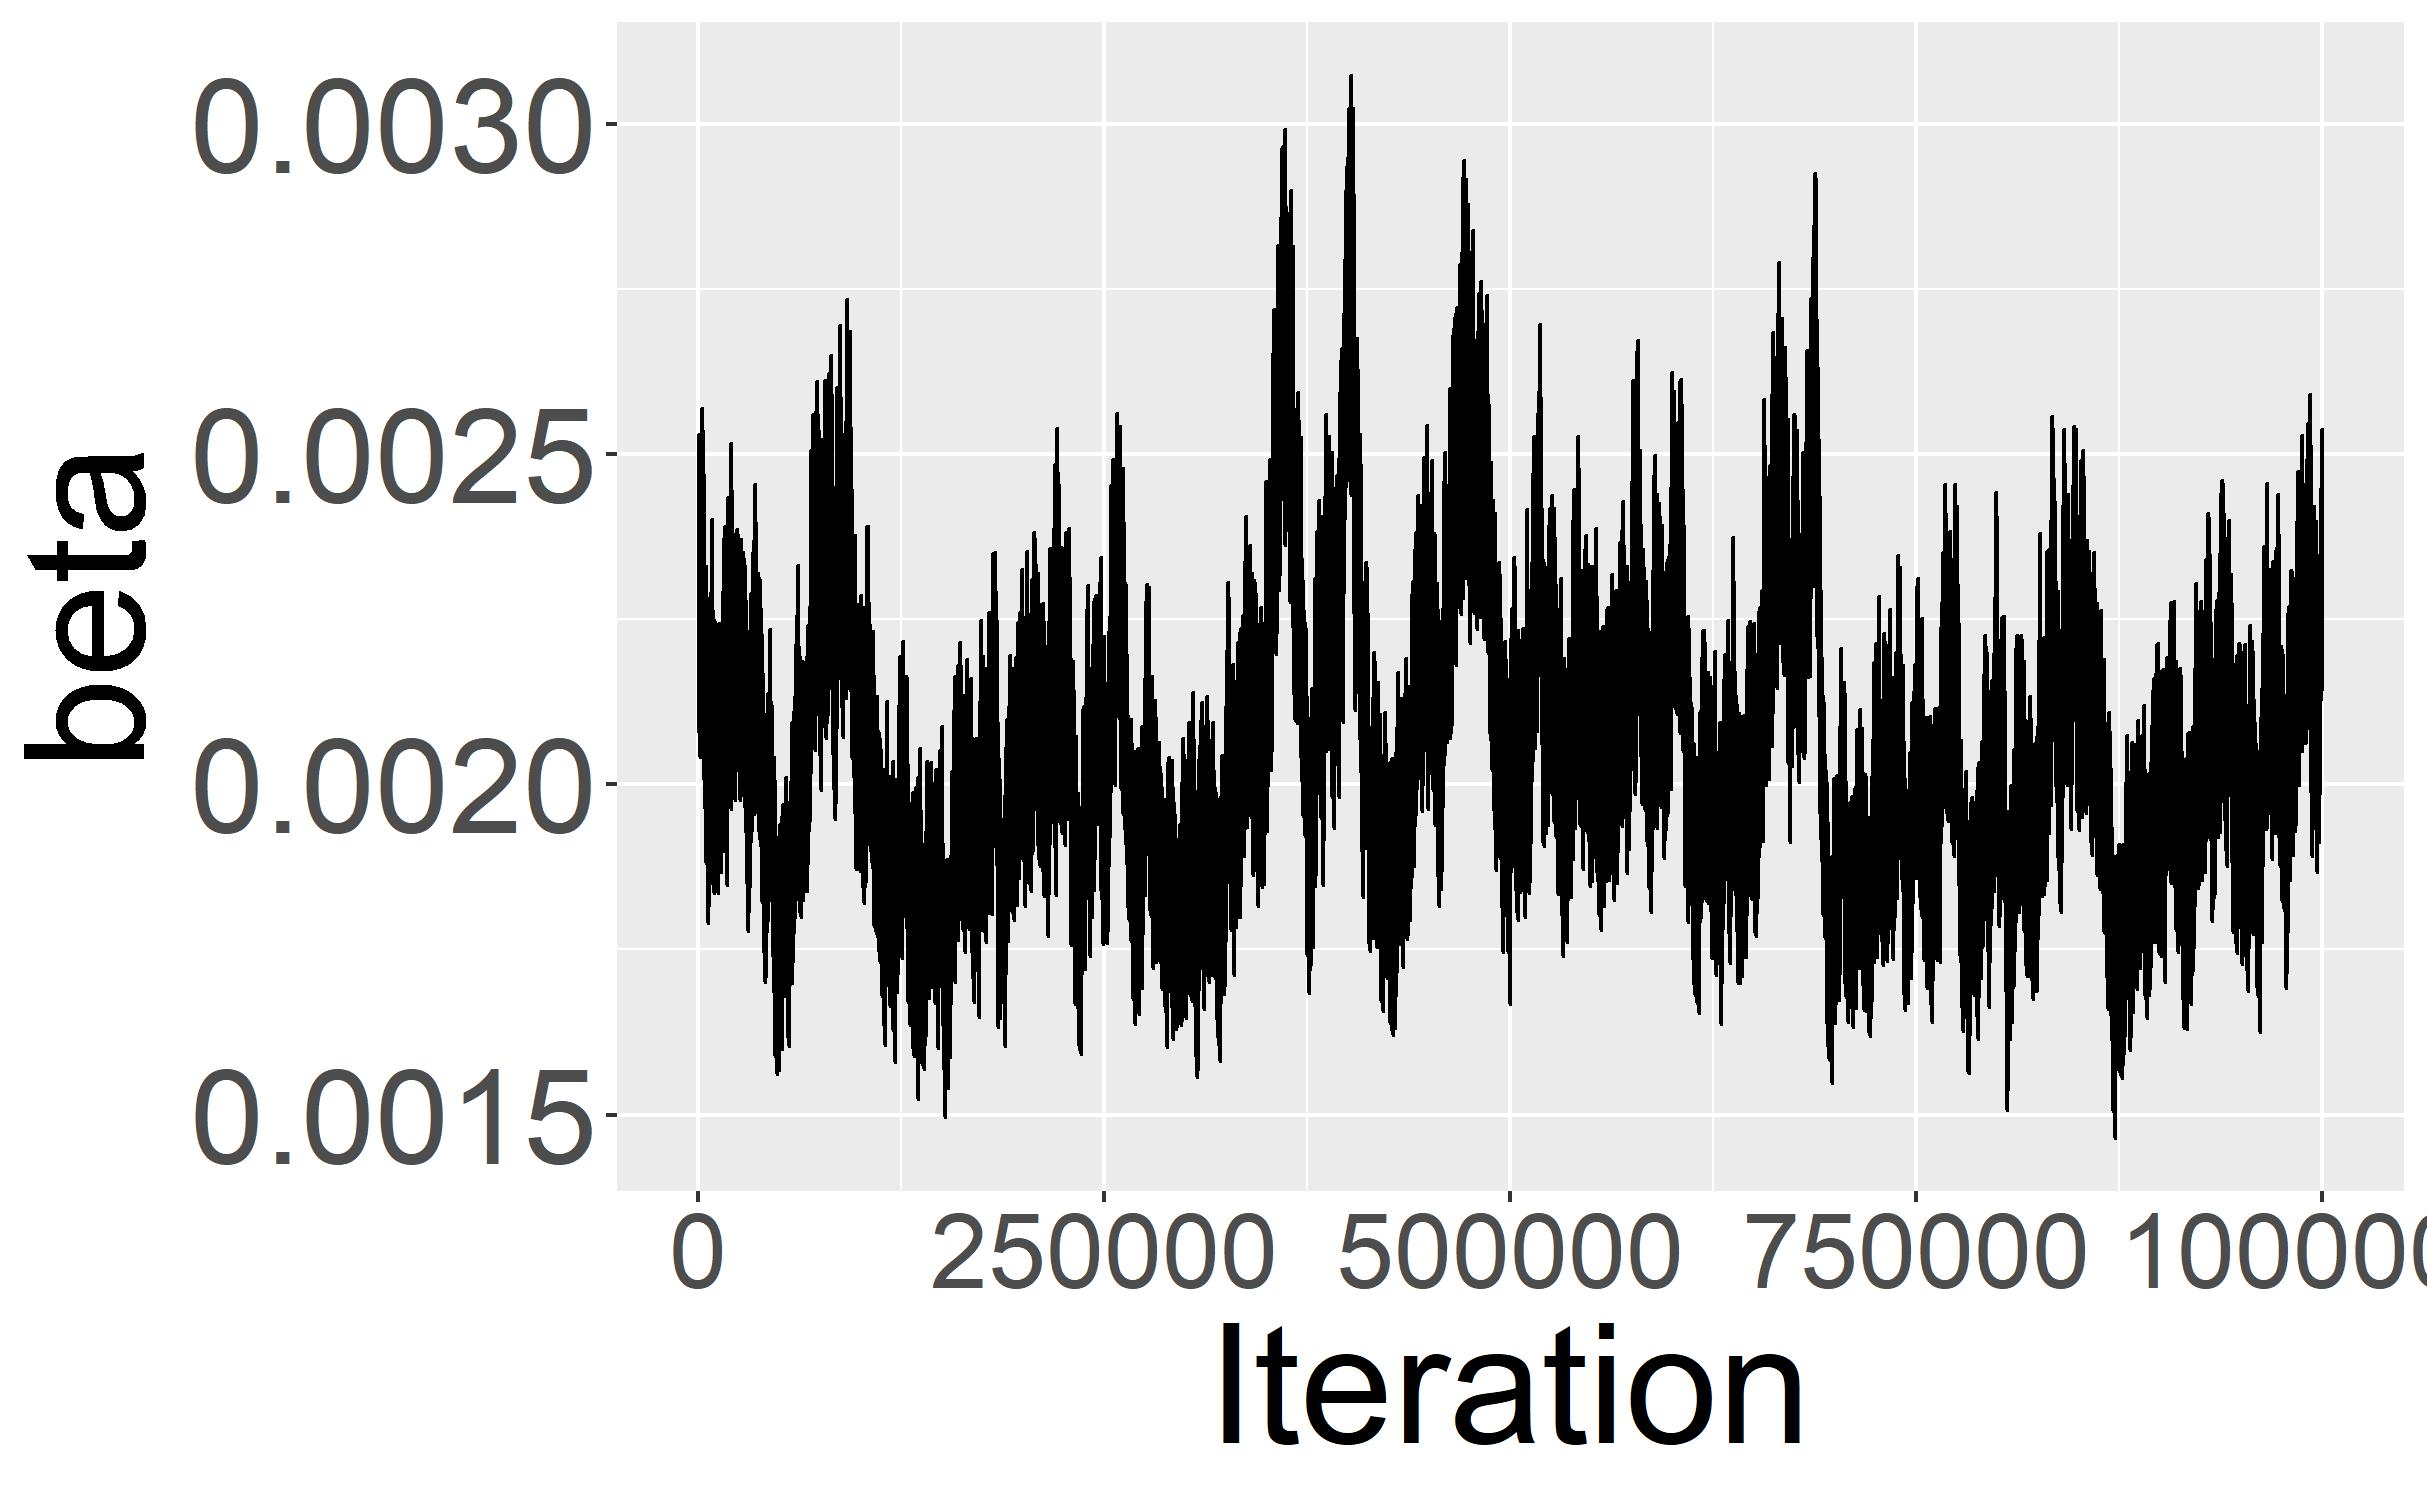
\includegraphics[width=\textwidth]{E6_no_burn_beta_tp_single.jpg}
			\caption{SSU DA-MCMC}
			\label{fig:E6_no_burn_beta_tp_single}
		\end{subfigure}
		\\
		\begin{subfigure}[b]{0.42\textwidth}
			\centering
			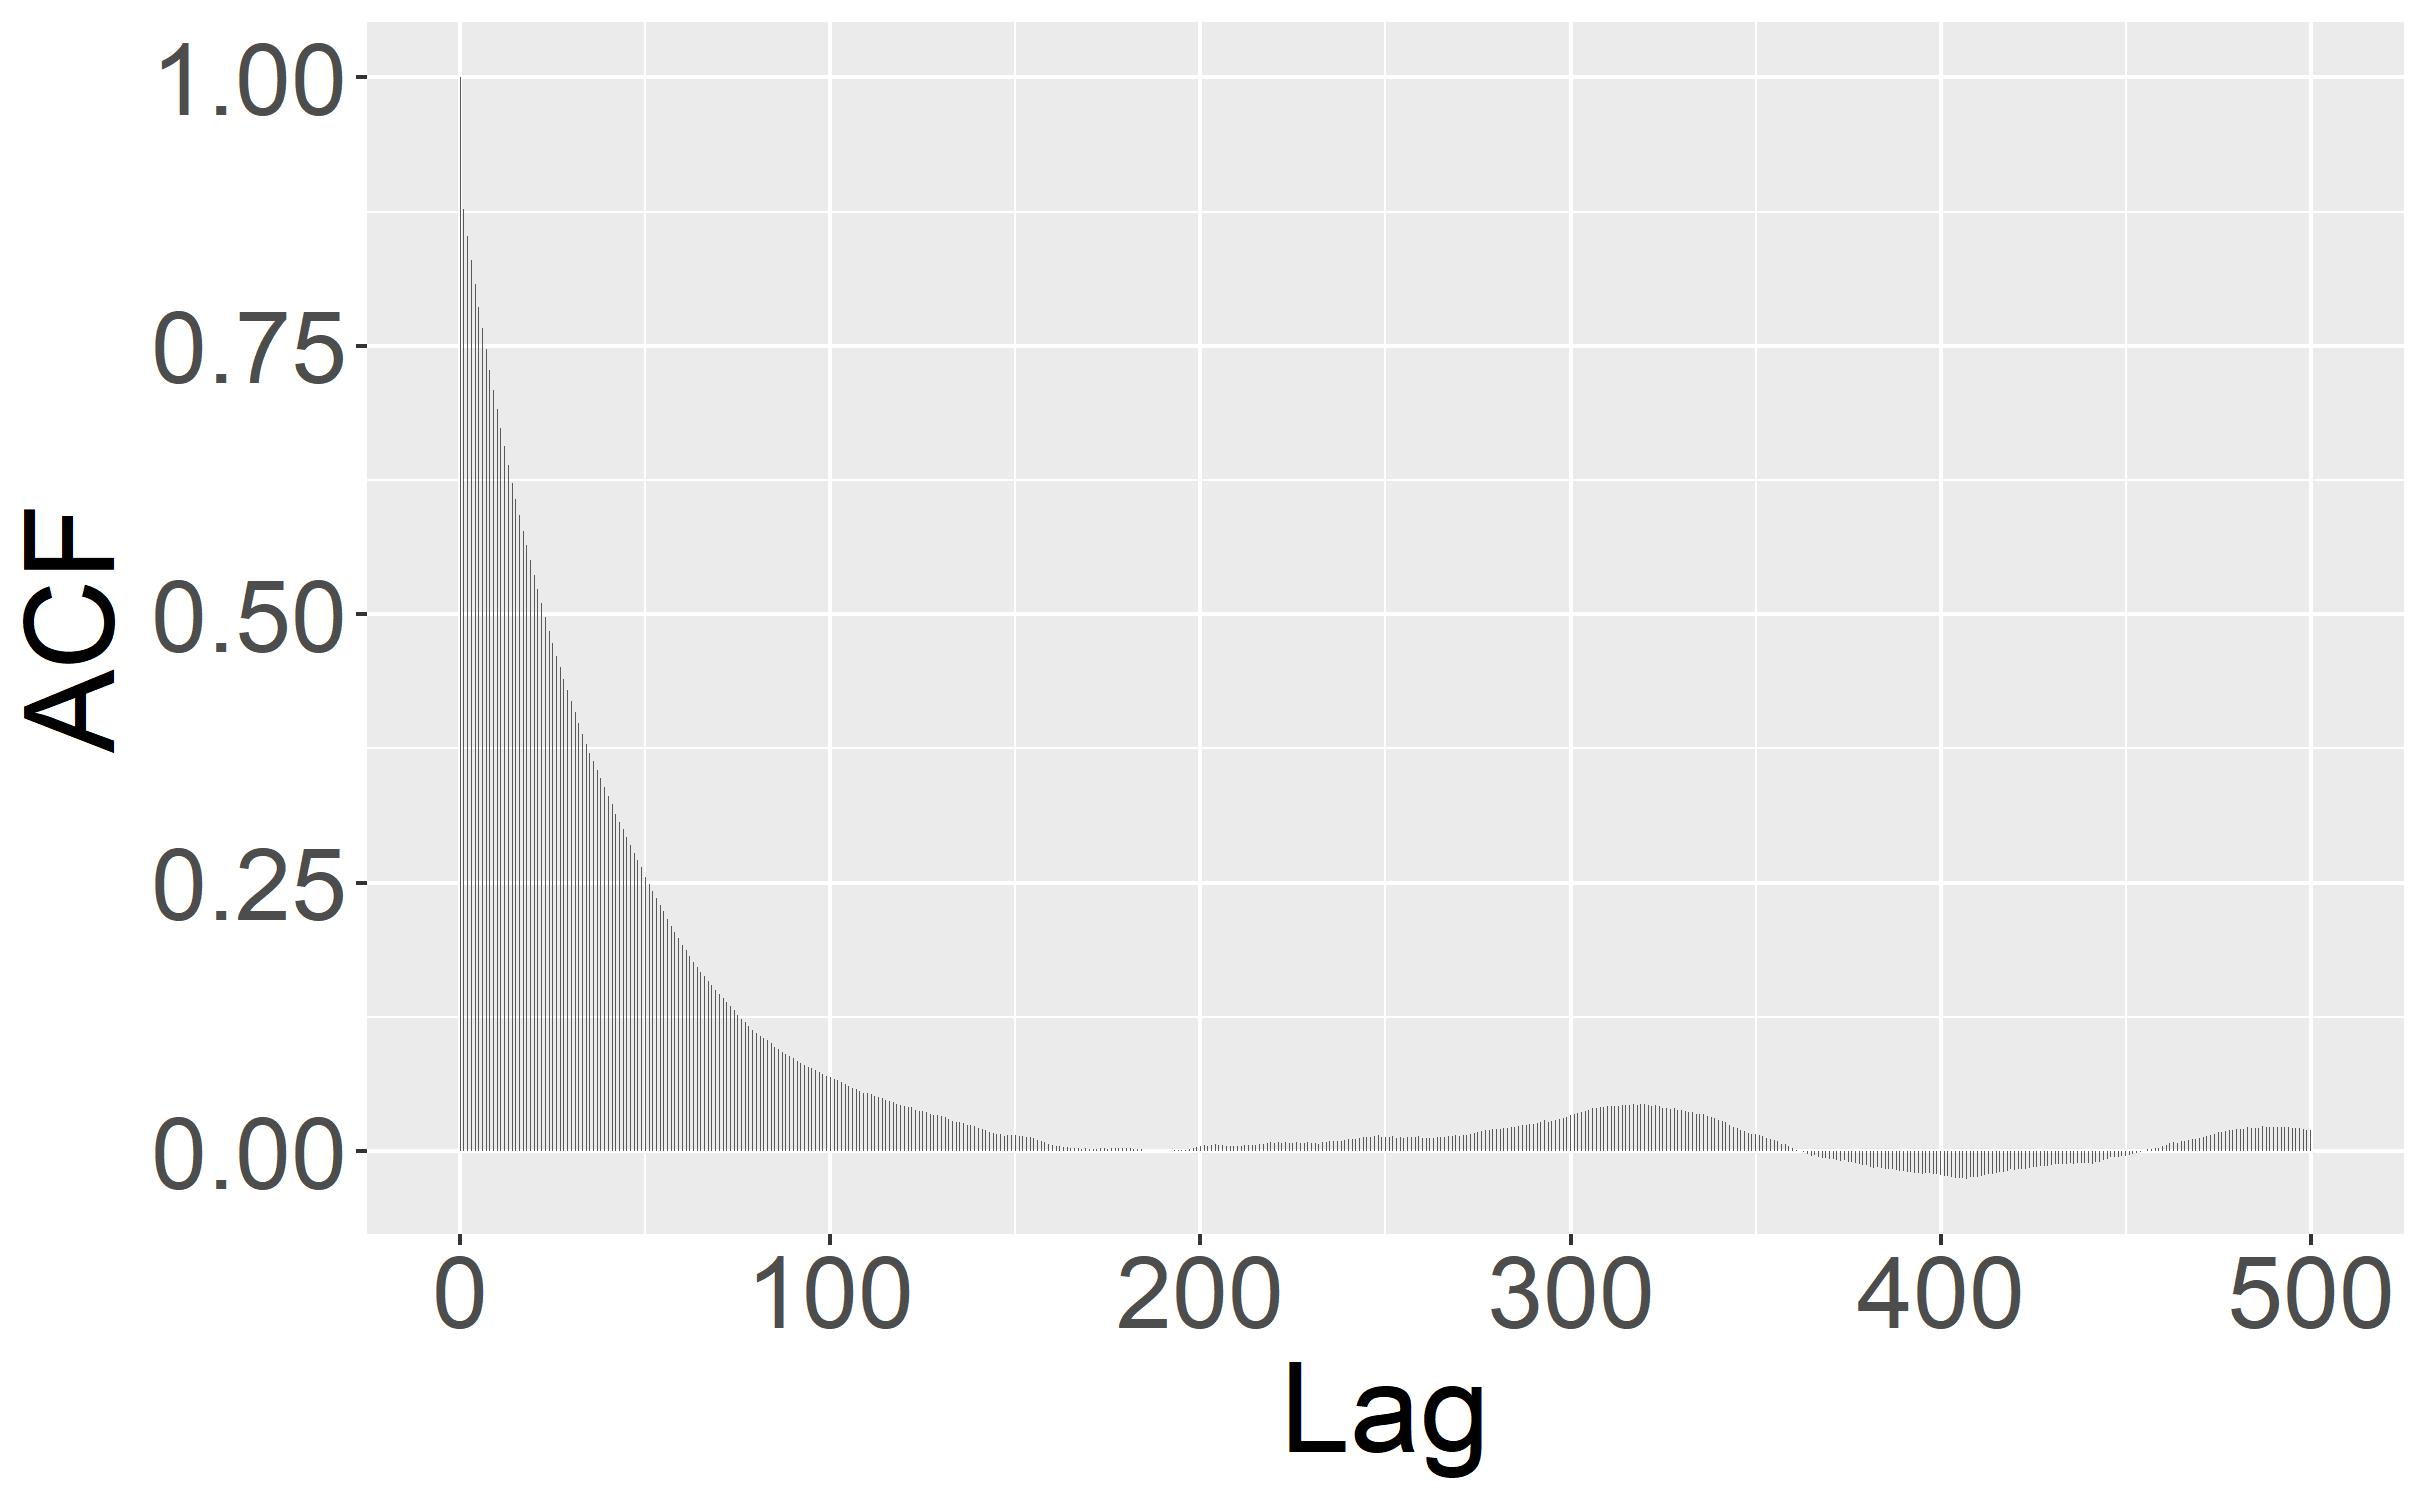
\includegraphics[width=\textwidth]{E6_burn_beta_acf_joint.jpg}
			\caption{DA-MCMC}
			\label{fig:E6_burn_beta_acf_joint}
		\end{subfigure}
		\hfill
		\begin{subfigure}[b]{0.41\textwidth}
			\centering
			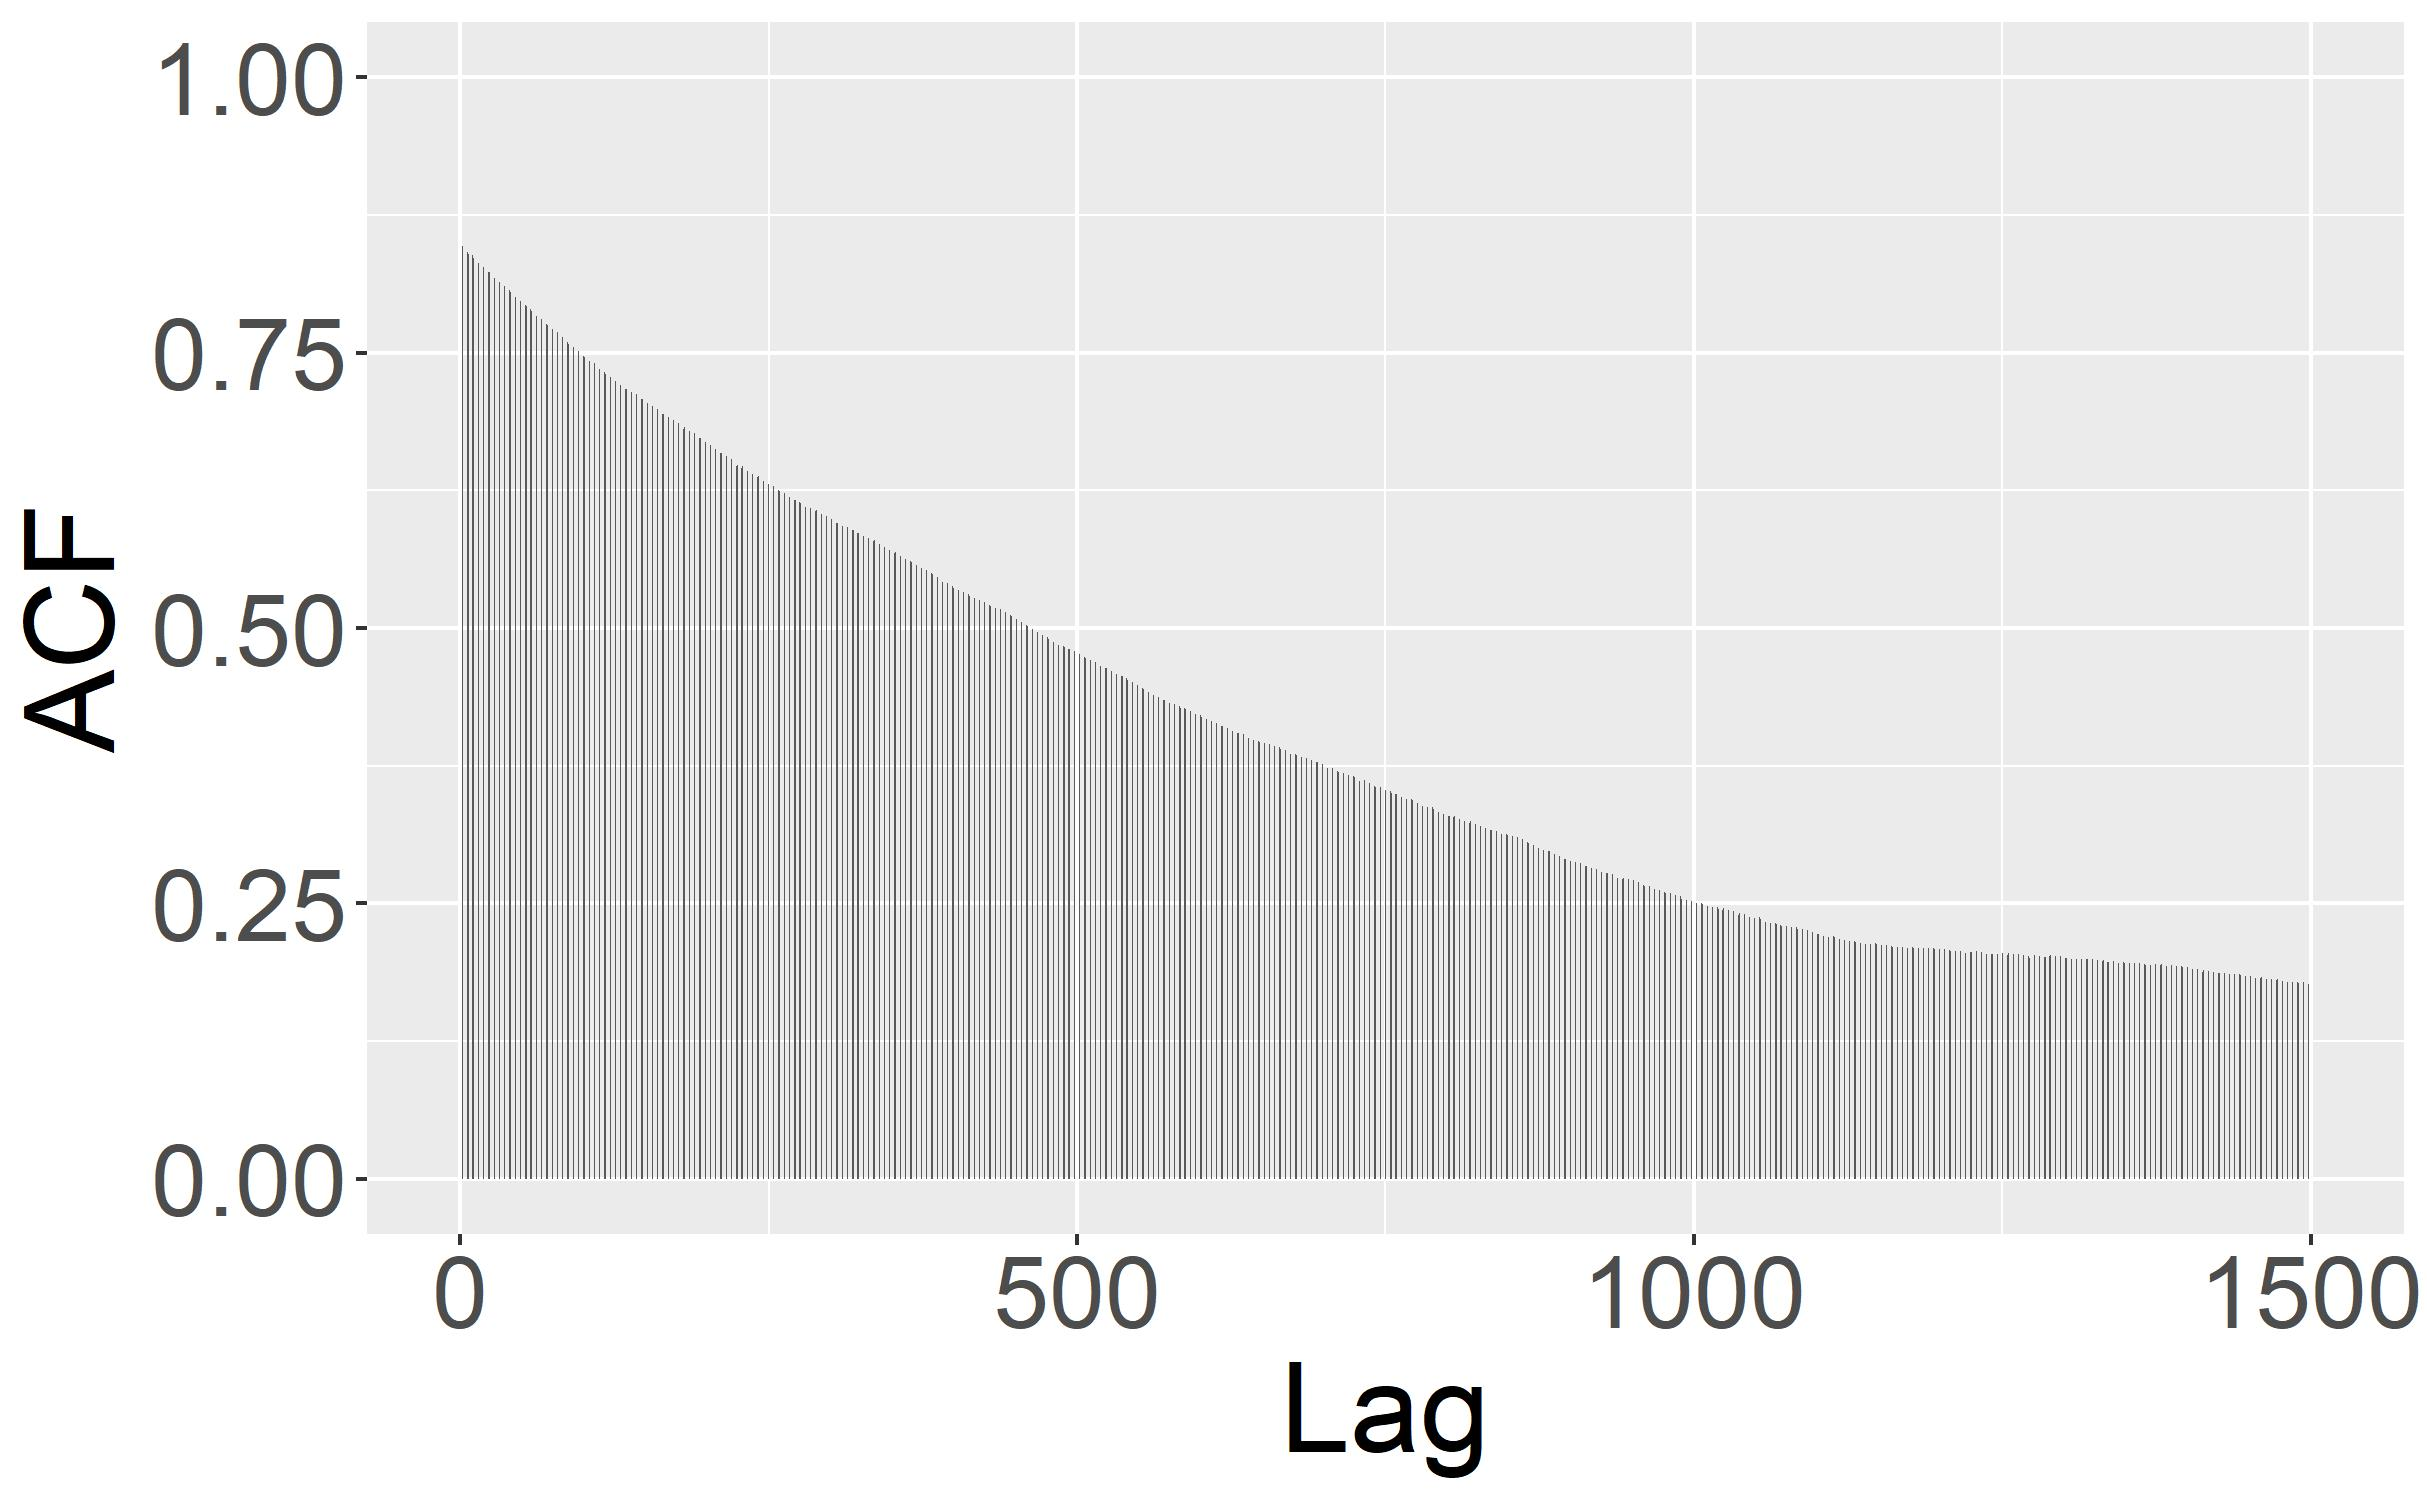
\includegraphics[width=\textwidth]{E6_burn_beta_acf_single.jpg}
			\caption{SSU DA-MCMC}
			\label{fig:E6_burn_beta_acf_single}
		\end{subfigure}
		\caption{Traceplots and auto-correlation functions of the proposed DA-MCMC and the SSU DA-MCMC for $\beta$.}
		\label{fig:E6}
	\end{figure}
	
	 \begin{table}
        \centering
        \begin{tabular}{ |C{2cm}| *{2}{C{3cm}}|}
            \hline
            Parameter & DA-MCMC & SSU DA-MCMC \\ 
            \hline
            $\beta$ & 0.20 & 0.01 \\ 
            $\gamma$ & 0.19 & 0.01 \\ 
            $R_0$ & 0.38 & 0.05 \\
            \hline
        \end{tabular}
        \caption{Effective sample size per second for for the proposed DA-MCMC and the SSU DA-MCMC.}
        \label{tab:E6}
    \end{table}
	
	\subsection{Ebola Outbreak in Gu\'eck\'edou, Guinea}
	\label{sec:ebo}
	%Outline: background; setup; results; table; figure
	
	We now turn to a case study concerning the Ebola outbreak in Western Africa.
	Between the end of $2013$ and $2015$, Guinea, along with several neighboring countries, experienced the largest outbreak of the Ebola virus disease in history. The virus, which has a fatality rate of $70\%$, was responsible for the death of almost $2,000$ people in Guinea alone.
	The outbreak is believed to have originated in the Gu\'eck\'edou prefecture of Guinea at the end of November $2013$ \cite{Baize.2014}. Weekly infection incidence counts are available for each prefecture for the $73$ weeks between the end of December $2013$ and May $2015$.
	The analysis serves to show that fast and exact Bayesian inference can be made regarding the Ebola pandemic with the proposed DA-MCMC algorithm instead of providing new insights into this outbreak or the Ebola virus in general.
	
	We fit the stochastic SIR model to these incidence counts for the Gu\'eck\'edou prefecture using the MCMC algorithm proposed in this article.
	For simplicity, we assume that the population of the prefecture forms a closed population, that the model's parameters remained constant throughout the outbreak and that the reported infections counts are exact.
	\ram{Justify these assumptions.}
	Applying the proposed DA-MCMC algorithm to stochastic epidemic models where these assumptions are relaxed is the subject of ongoing research.
	The population size is set to $n = 292000$, the estimated population of the Gu\'eck\'edou prefecture in $2014$.
	The units of time correspond to ``days" in the analysis and $t=0$ corresponds to Monday December 30, 2013, the first day of the observation period.
	Since the first documented infection occurred late November \cite{Baize.2014}, one month before the first reported incidence count, we set $I(0) = 5$.
	
	The Markov chain is run for $1$ million iterations and the event times of $\rho=10\%$ of the individuals are updated each iteration. The initial values of the parameters are set to $(\beta^{(0)}, \gamma^{(0)}) = (10^{-7}, 0.05)$ and the conjugate distributions in Equation \ref{eq:pri} are used as priors with $a_{\beta} = b_{\beta} = a_{\gamma} = b_{\gamma} = 1$ to make them weakly informative. Even for such a large population, the total run time of the algorithm was less than $100$ minutes on a personal laptop.
	The Metropolis-Hastings step for the latent data proposals achieves a healthy $20.1\%$ acceptance rate, and the first $50,000$ iterations of the Markov chain are discarded as a burn-in.
	Figure \ref{fig:ebola} shows the marginal posterior distributions $\gamma$, whose means is $0.109$. This indicates that people remained infectious for around $9$ days on average, which is consistent with existing literature. 
	%As noted by numerous authors, conditionally on partially observed data, the parameters $\beta$ and $\gamma$ appear positively correlated.
	%The posterior distribution of $R_0$ is unimodal, relatively symmetric, and centered around $1$. A basic reproduction number close to $1$ is consistent with an outbreak that lasted several months without infecting the majority of the population.
	
	\begin{figure}
		\centering
		\begin{subfigure}[b]{0.45\textwidth}
			\centering
			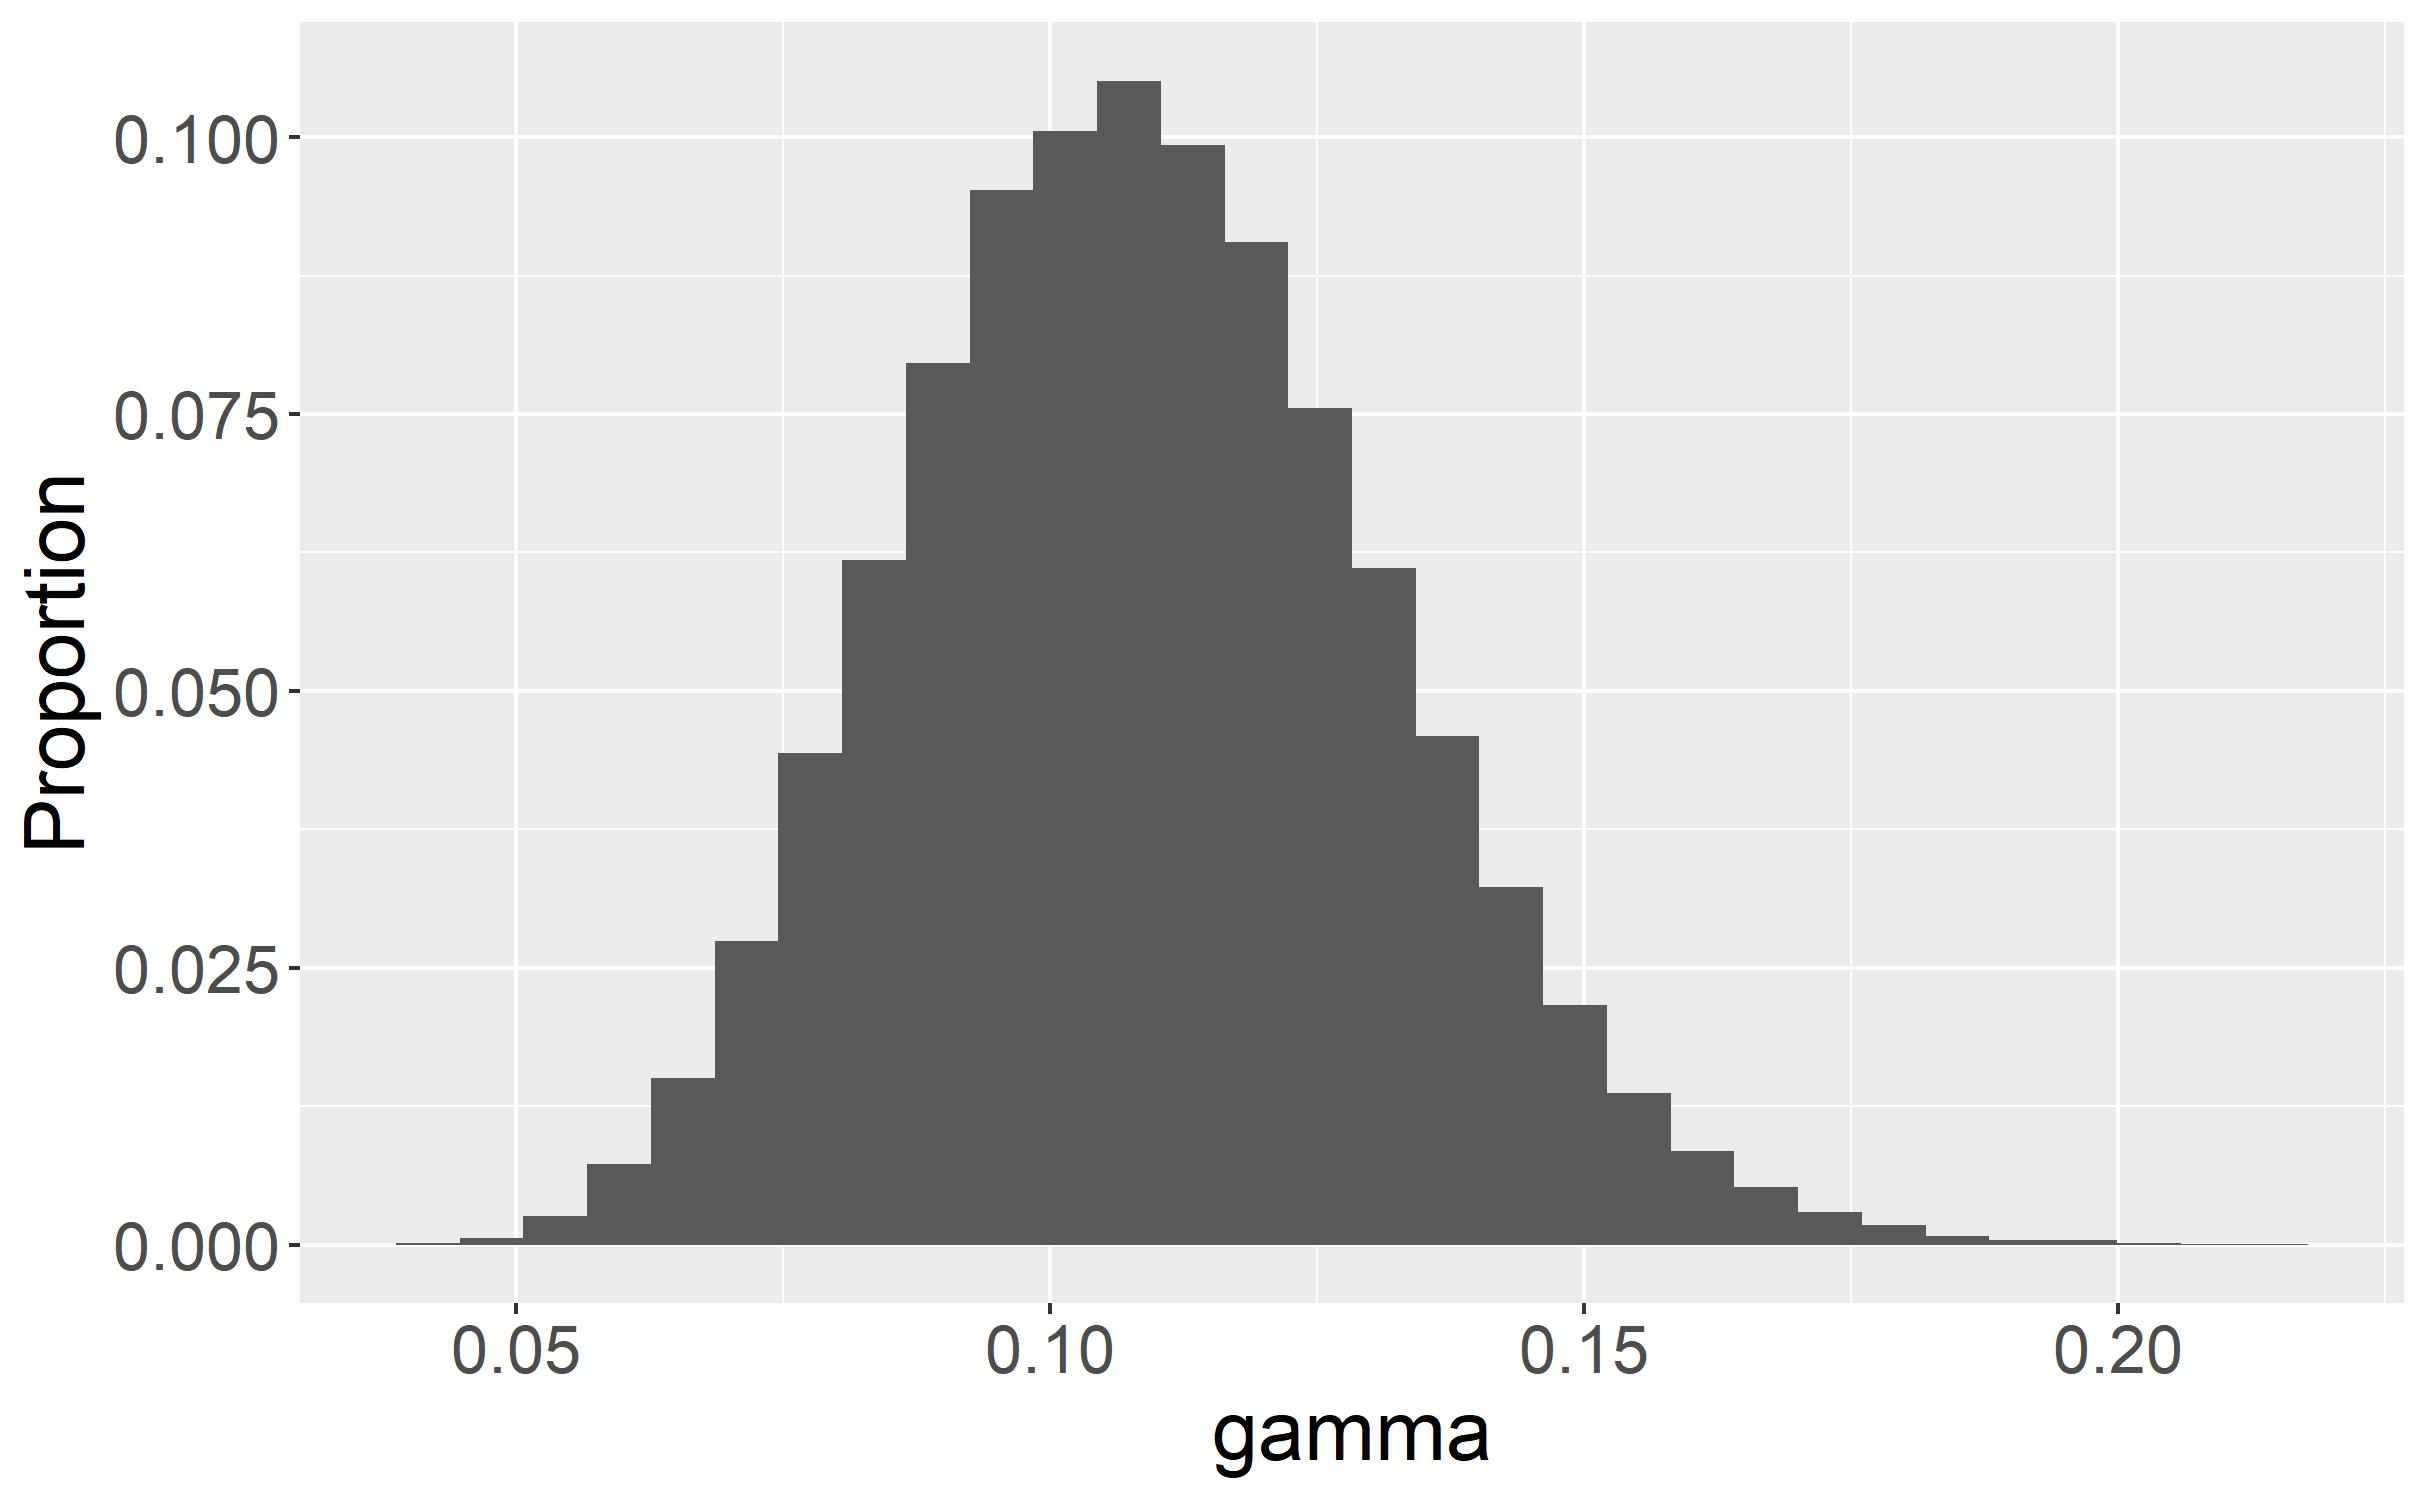
\includegraphics[width=\textwidth]{E5_gamma_hist}
			\caption{Histogram of $\gamma$}
			\label{fig:E5_gamma_hist}
		\end{subfigure}
		\hfill
		\begin{subfigure}[b]{0.49\textwidth}
			\centering
			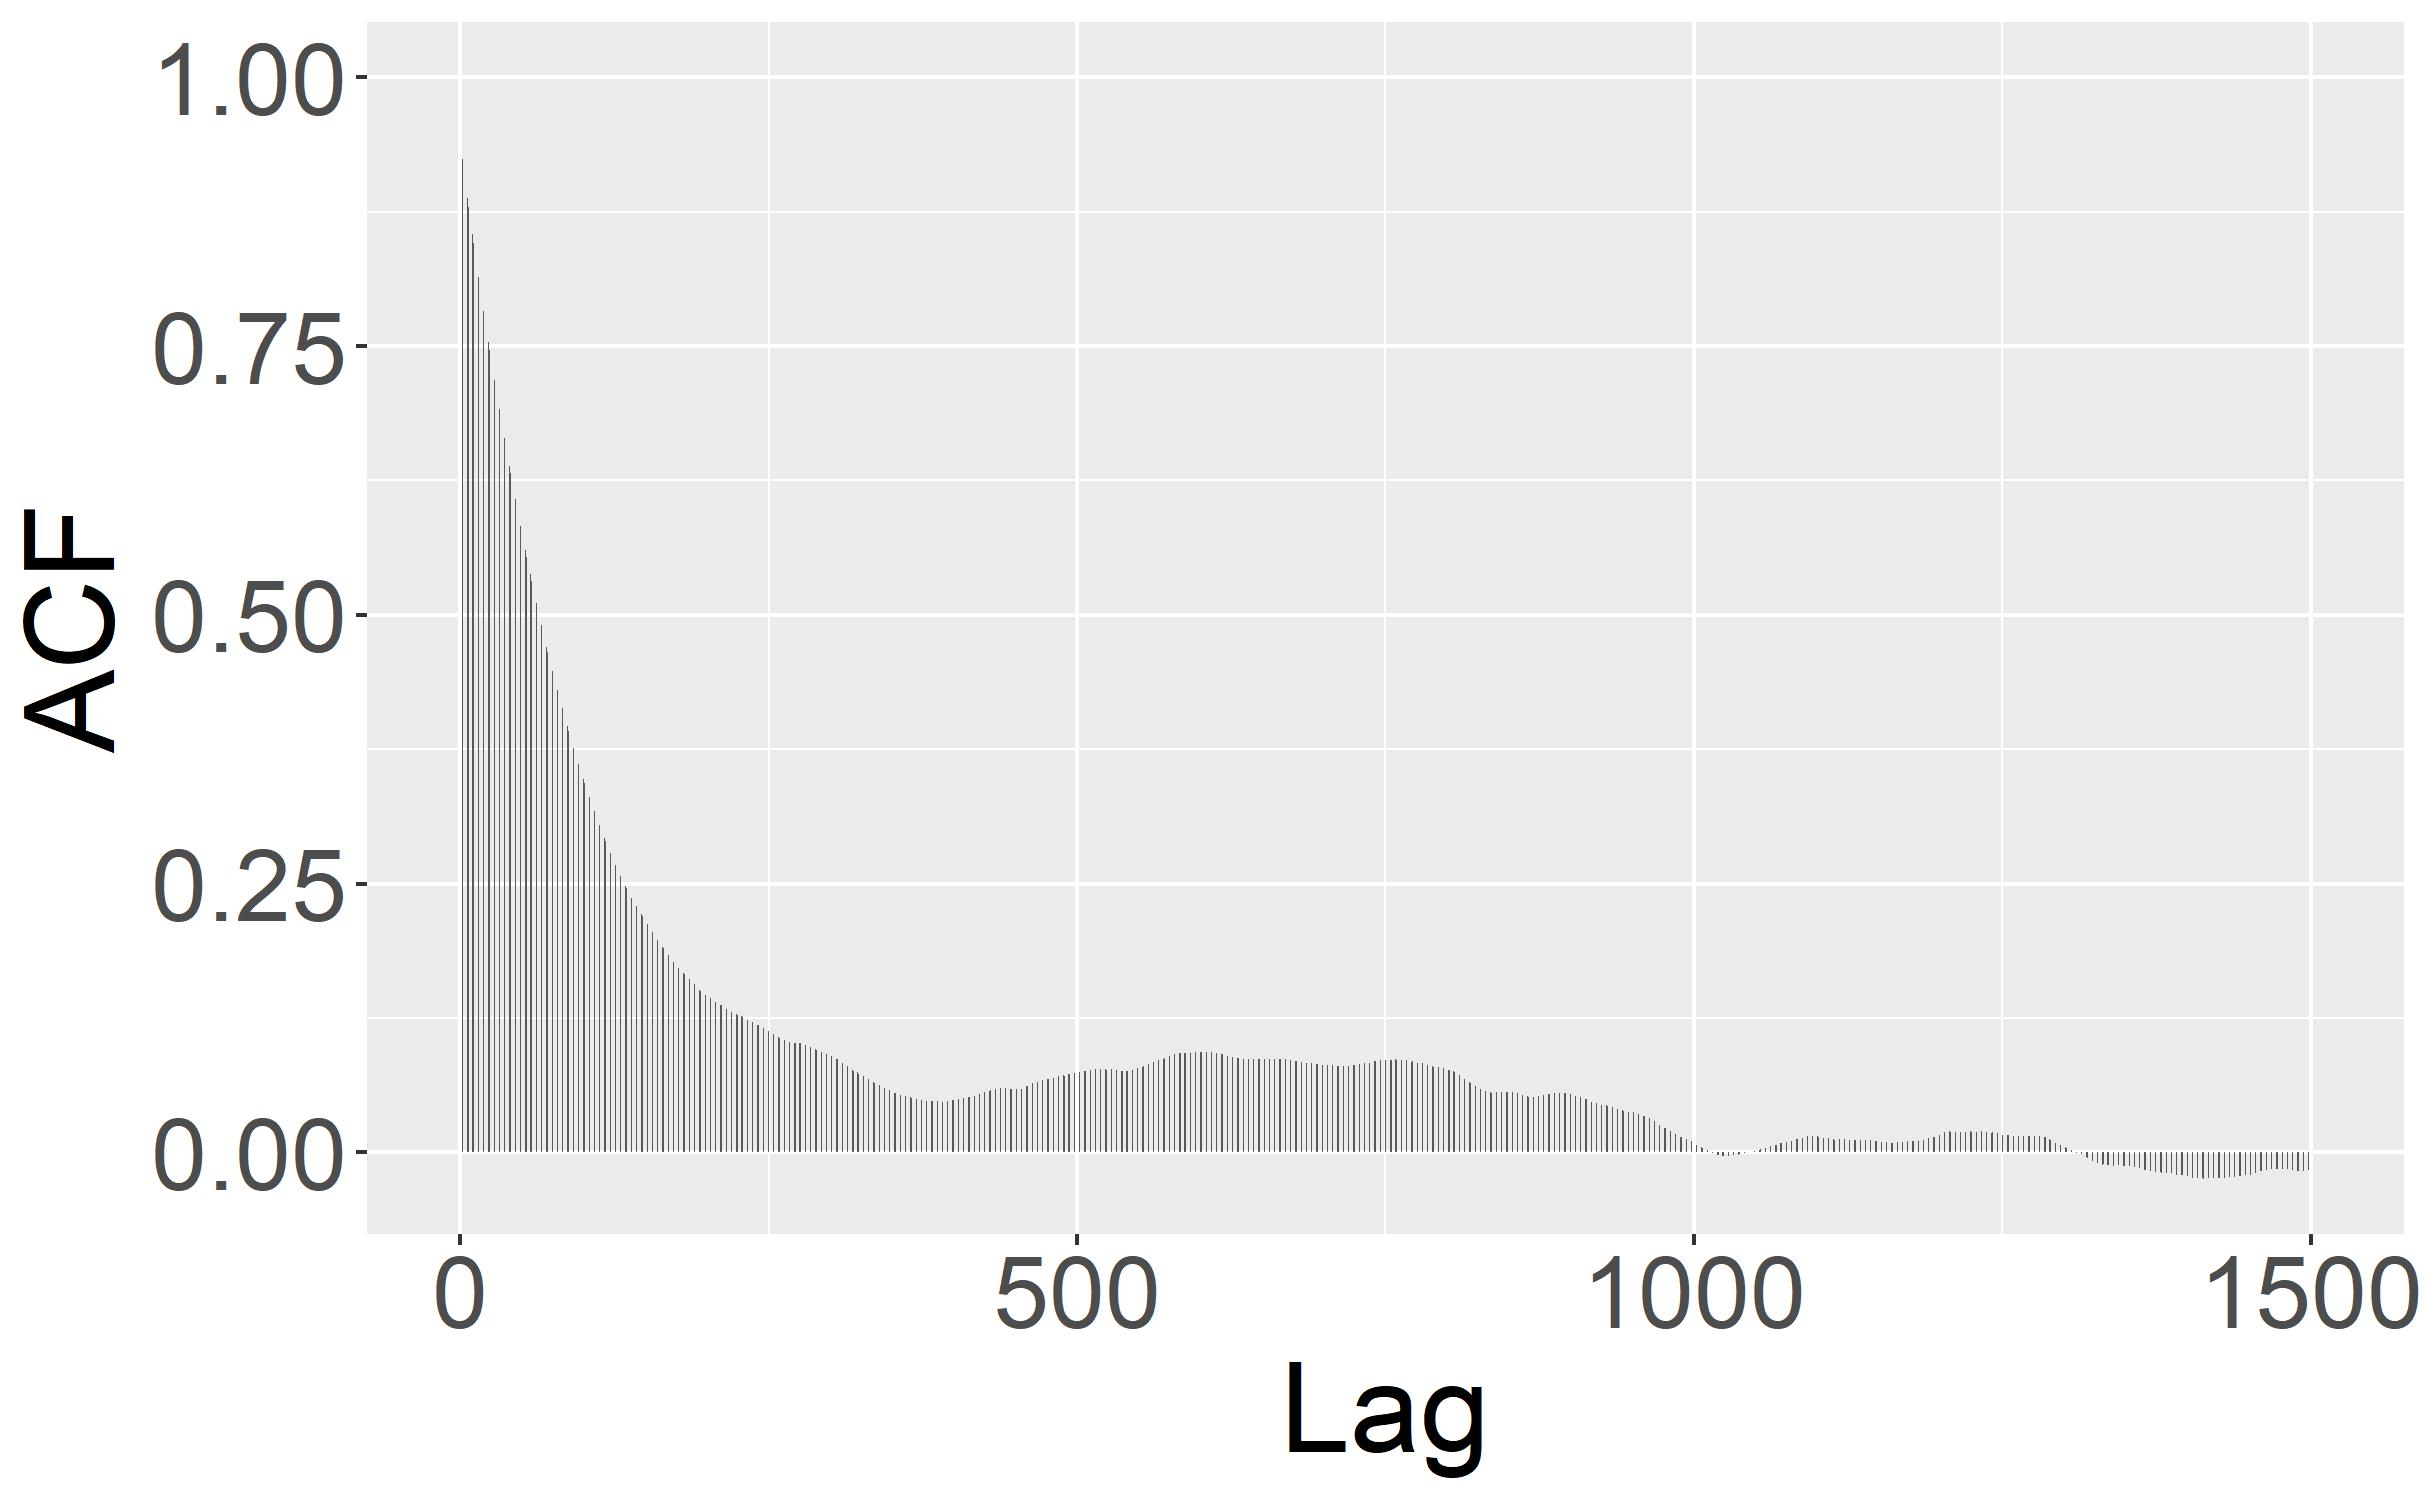
\includegraphics[width=\textwidth]{E5_gamma_acf}
			\caption{Posterior density of $R_0$.}
			\label{fig:density_R0}
		\end{subfigure}
		\caption{Marginal posterior distribution of $\gamma$ and its auto-correlation function for the Gu\'eck\'edou prefecture.}
		\label{fig:ebola}
	\end{figure}
	
	\section{Discussion and Conclusion}
	\label{sec:dis}
	The method proposed in this article enables the classical Metropolis-Hastings algorithm to be an efficient method to conduct full posterior inference of the stochastic SIR model given only incidence data. Existing attempts using Markov chain Monte Carlo either mix poorly or do not scale to populations of more than a few hundred individuals, while methods relying on forward simulation are limited to moderate-sized outbreaks and may suffer from degeneracy issues on a case-by-case basis depending on the amount of missing data. 	Moreover, the simplifying assumptions in \cite{Fintzi.2020} or the approximate-Bayesian-computation framework of \cite{McKinley.2018}, which compromise targeting the exact posterior for computational reasons, generate biased estimates that may lead to spurious conclusions. Instead, our data-augmented algorithm enables fast and exact inference, even for large outbreaks, and leverages a well-studied, transparent MCMC framework. %Most existing inferential methods for epidemic stochastic models are only applicable to prevalence data. To our knowledge, our algorithm is the first that permits exact Bayesian inference given incidence data.
	
	Central to the success of the DA-MCMC algorithm is an efficient proposal scheme that swiftly explores the latent space of epidemic paths that are compatible with the observed data. The PD-SIR process possesses three features that yield such an efficient algorithm. First, generating a PD-SIR process is extremely fast; it only requires the simulation of truncated exponential distributions, which can efficiently be realized via the inverse-CDF method. Moreover, the individual infection rates are only updated $K$ times, as opposed to after each event as in the SIR model. Second, generating a PD-SIR process that is constrained to be compatible with the observed incidence data can be done at no additional cost; in contrast, generating a SIR process compatible with the observed data would be prohibitively slow \cite{Hobolth.2009}. Third, the dynamics of the PD-SIR process closely resemble those of the SIR process: the removal dynamics are identical and, for short resetting intervals, the infection dynamics are also very similar in the two processes.
	
	The first two features make the algorithm extremely fast. While existing data-augmented MCMC algorithms have only be applied to populations of a few hundred of individuals, the analysis of the Ebola outbreak in Gu\'eck\'edou shows that our algorithm can be applied to populations of up to $150,000$ individuals, generating tens of thousands of posterior samples in a reasonable amount of time.	
	The latter feature of the PD-SIR process enables the algorithm to update a large portion of the augmented data in each iteration while maintaining a healthy acceptance rate. As a result, the Markov chain makes large jumps in the latent space and has very good mixing properties. In contrast, existing DA-MCMC algorithms keep most of the latent space fixed across iterations \cite{Gibson.1998, ONeill.1999, Fintzi.2017} and their Markov chains therefore mix much more slowly.
	
	The algorithm possesses a tuning parameter $\rho$ that determines the portion of the augmented data being updated each iteration. Larger values for $\rho$ enable the chain to make larger steps in the latent space but can result in a low acceptance rate, while smaller values of $\rho$ result in a higher acceptance rate but constrain the chain to make small jumps. Depending on the size of the population, different values of the tuning parameter are optimal. To find a value that optimizes the mixing properties of the chain, one can use several short runs of the algorithm with different values for $\rho$ and select the value that yields the lowest auto-correlation function (ACF). Since the run time of the algorithm increases with $\rho$, one could also look at the effective sample size per unit of time. For instance, for populations of a few hundred individuals, we observed that updating the entire augmented data ($\rho=1$) yields the lowest ACF. In this case, the current and proposed augmented data are independent conditionally on the current value of the parameters.
	
	The DA-MCMC algorithm proposed in this article is specific to the stochastic SIR model, which is arguably a simplistic representation of the spread of disease. The model relies on assumptions such as perfect reporting, constant infection rates, homogeneously mixing population and exponentially-distributed infectious periods. In future work, we will present applications of our DA-MCMC algorithm to processes where these assumptions are relaxed. In particular, we are considering extensions to epidemic models with under-reporting \cite{Fintzi.2017}, non-Markovian dynamics \cite{Streftaris.2002}, and a time-varying infection rate \cite{Kypraios.2018}.
	
	\ram{modelling the infection rate over time seems necessary for EBola data.}
	
	\appendix
	
	\section{Distribution of Death Times in Linear Death Process}
	\label{app:ldp}
	
	Theorem \ref{theo:ldp} was first proved by by \cite{Neuts.1971}. Ross provides a simpler proof which we now give.
	
	\begin{proof}
	Consider a linear pure death process with $n$ particles and individual death rate $\mu$.
	Let $T_i$ be the time of the $i$th death. Then $W_1 = T_1 \sim \Exp(n\mu)$ and $W_i = T_i - T_{i-1} \sim \Exp((n-1)\mu)$ independently. Let $N$ be the number of deaths by time $t$. Then, 
	\begin{align*}
		& f(T_1 = t_1, \dots, T_N = t_N | N) \\
		& \propto f(T_1 = t_1, \dots, T_N = t_N, T_{N+1} > t) 1\{T_N < t\}\\
		& \propto f(W_1 = t_1, W_2 = t_2 - t_1, \dots, W_N = t_N - t_{N-1}, W_{N+1} > t - t_N) 1\{T_N < t\}\\
		& \propto \exp\{-n\mu t_1\} \exp\{-(n-1)\mu(t_2-t_1)\}\dots \exp\{-(n-N)\mu(t - t_N)\} 1\{T_N < t\}\\
		& \propto \exp\{-\mu t_1\}\exp\{-\mu t_2\} \dots \exp\{-\mu t_N\} 1\{T_N < t\}
	\end{align*}
	which corresponds to the kernels of independent exponential distribution truncated above by $t$.
	
	\end{proof}
	
	\section{Proofs}
	\label{app:uni}
	% 	We show that the state space $\chi = \chi_{\theta}\times\chi_{\z}$ of the Markov chain $\{(\theta, \z)^{(i)}\}_i$ is a small set for the transition kernel $P$, that is, there exists a probability measure $\nu$ on the $\sigma$-algebra $\sigma(\chi)$ such that
	% 	$$\beta \nu(.) \le P^m(x,.), \forall x\in \chi.$$
	% 	for some constants $m \ge 1$ and $\beta > 0$.
	% 	By Proposition 2 in \cite{Tierney.1994}, this implies that the Markov chain $\{(\theta, \z)^{(i)}\}_i$ is uniformly ergodic and therefore satisfies
	% 	$$
	% 	\Vert P^n(x,.)-\pi(.)\Vert_{TV} \le M r^n
	% 	$$
	% 	for some finite $M$ and positive constant $r<1$, where $\Vert \mu \Vert_{TV}$ denotes the total variation norm of the measure $\mu$.
	
	% 	The following three lemmas are used to show this result.
	
	
	% 	% Gamma 1
	% 	\begin{lemma}
	% 		\label{pro:ga1}
	% 		Let $Ga(x;a,b)$ denote the density of a gamma distribution with shape $a$ and rate $b$ evaluated at $x$. Then
	% 		\begin{equation}
	% 			\label{eq:ga1}
	% 			\inf_{0\le \beta\le B} Ga(x;a,b+\beta) = 
	% 			\begin{cases}
	% 				Ga(x;a,b), & x<x_a^* \\ Ga(x;a,b+B), & x\ge x_a^*
	% 			\end{cases}
	% 		\end{equation}	
	% 		where $x_a^*=\frac{a}{B}\log\left( 1+\frac{B}{b}\right) $. Moreover,
	% 		\begin{equation}
	% 			\label{eq:ga2}
	% 			\inf_{0\le \alpha\le A} Ga(x;a+\alpha,b) = 
	% 			\begin{cases}
	% 				Ga(x;a,b), & x>x_b^* \\ Ga(x;a+A,b), & x\le x_b^*
	% 			\end{cases}
	% 		\end{equation}
	% 		where $x_b^*=\frac{1}{b}\left[ \frac{\Gamma(a+A)}{\Gamma(a)}\right]^{1/A} $.
	% 	\end{lemma}
	
	%Proof of Lemma \ref{pro:ga1}.
	
	
	\begin{figure}
		\centering
		\begin{subfigure}[b]{0.45\textwidth}
			\centering
			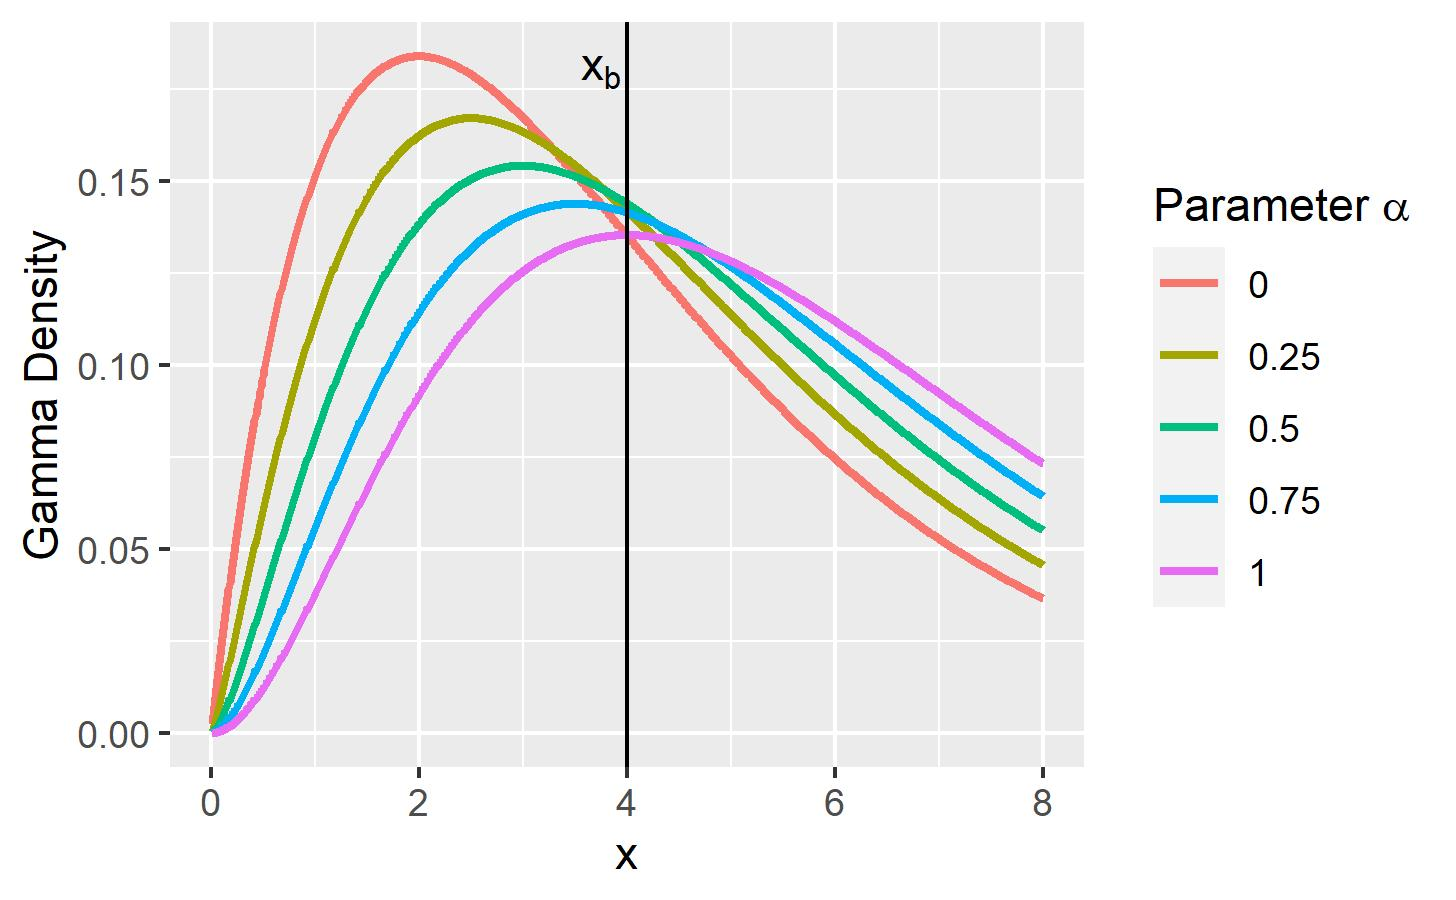
\includegraphics[width=\textwidth]{gamma_minorization_1a.jpg}
			\caption{$\alpha \in [0, 1]$, $\beta=0$}
			\label{fig:gam1a}
		\end{subfigure}
		\hfill
		\begin{subfigure}[b]{0.49\textwidth}
			\centering
			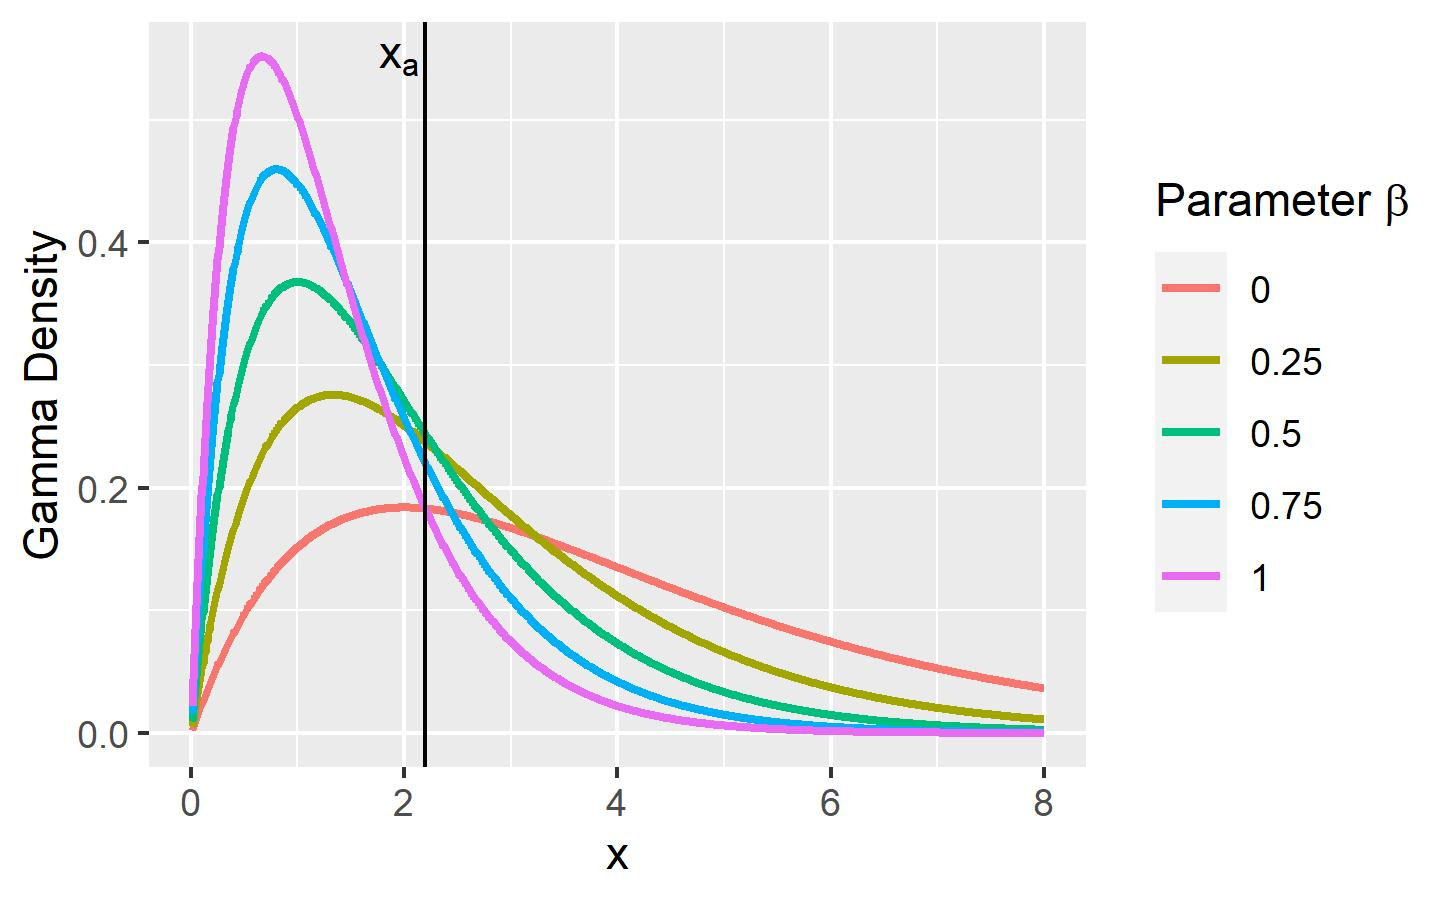
\includegraphics[width=\textwidth]{gamma_minorization_1b.jpg}
			\caption{$\alpha = 0$, $\beta \in [0, 1]$}
			\label{fig:gam1b}
		\end{subfigure}
		\caption{Example of minorization of the density of a gamma distribution $Ga(2+\alpha, 0.5+\beta)$ for $\alpha$ and $\beta$ separately.}
		\label{fig:gam1}
	\end{figure}
	
	
	% Gamma 2
	Proof of Lemma \ref{pro:ga2}: % can be used to minorize a density of the form
	% \begin{equation}
	% 	\label{eq:ga}
	% 	Ga(x;a+\alpha,b+\beta) = \frac{(b+\beta)^{a+\alpha}}{\Gamma(a+\alpha)}x^{a+A-1}\exp\{-x(b+B)\}, \quad 0\le\alpha\le A, 0\le\beta\le B.
	% \end{equation}
	% over $\alpha$ and $\beta$ for each value of $x$. We can show the following.
	% \begin{lemma}	
	% 	\label{pro:ga2}
	% 	For a fix $x>0$, the density $Ga(x;a+\alpha,b+\beta)$ is minimized by $(\alpha, \beta) \in \{(A, 0), (0, B)\}$, the minimizing set of values depending on $x$. In particular,	
	% 	$$\inf_{\begin{aligned}
	% 			0\le \alpha\le A \\ 0\le \beta\le B
	% 	\end{aligned}}Ga(x;a+\alpha,b+\beta) = 
	% 	\begin{cases}
	% 		Ga(x;a+A,b)                     , & x<x_a         \text{ or } x<x_{a+A}^* \vee x_b^*\\
	% 		Ga(x;a,b+B)                     , & x_{a+A}^* < x \text{ or } x_a^* \wedge x_{b+B}^* < x\\
	% 		\min\{Ga(x;a+A,b), Ga(x;a,b+B)\}, & x_a^* \wedge x_b^*\le x < x_{a+A}^* \vee x_{b+B}^*\\
	% 	\end{cases}$$
	% \end{lemma}
	
	\begin{proof}
		Given $x>0$, \ref{eq:ga1} shows that for a fixed $\alpha$, $\beta \in \{0, B\}$ is the minimizer of \ref{eq:ga}, and \ref{eq:ga2} shows that for a fixed $\beta$, $\alpha \in \{0, A\}$ is the minimizer of \ref{eq:ga}. This implies that for a fixed $x>0$, \ref{eq:ga} is minimized by $(\alpha, \beta) \in \{(0,0), (A, 0), (0, B), (A,B)\}$.
		
		A case-by-case analysis of the nine possibilities
		$$(x<x_a^*; x_a^*<x<x_{a+A}^*; x_{a+A}^* < x )\times(x<x_{b+B}^*; x_{b+B}^*<x<x_b^*; x_b^* < x)$$
		is presented in Table \ref{tab:ga9} and shows that it is sufficient to consider $(\alpha, \beta) \in \{(A, 0), (0, B)\}$.
		
		\begin{table}[H]
			\centering
			\begin{tabular}{l|c c c}
				& $x<x_a^*$  & $x_a^*\le x<x_{a+A}^*$ & $x_{a+A}^* < x$ \\ \hline
				$x<x_b^*$              & $(a+A, b)$ & $(a+A, b)$             &                 \\
				$x_b^*\le x<x_{b+B}^*$ & $(a+A, b)$ &  ad hoc                & $(a, b+B)$      \\
				$x_{b+B}^* < x$        &            & $(a, b+B)$             & $(a, b+B)$
			\end{tabular}
			\caption{Values of $(\alpha, \beta)$ that minimize $Ga(x;a+\alpha,b+\beta)$ for different values $x$.}
			\label{tab:ga9}
		\end{table}
		
		The two empty entries in Table \ref{tab:ga9} correspond to impossible configurations. Indeed, $x_b^* > x_a^*$ and $x_{a+A}^* > x_{b+B}^*$ for all $a, A, b, B$ since
		$$
		\frac{x_b^*}{x_a^*} = \dfrac{\left(\frac{\Gamma(a+A)}{\Gamma(a)}\right)^{1/A} b^{-1} }{a B^{-1} \log\left( 1+B/b\right)} = \dfrac{\left(\frac{\Gamma(a+A)}{\Gamma(a)}\right)^{1/A}}{a} \dfrac{B/b}{\log\left( 1+B/b\right)} = \dfrac{\Gamma_{a,a+A}}{a} \dfrac{B/b}{\log\left( 1+B/b\right)} \ge 1
		$$
		and
		$$
		\frac{x_{b+B}^*}{x_{a+A}^*} = \dfrac{\left(\frac{\Gamma(a+A)}{\Gamma(a)}\right)^{1/A} (b+B)^{-1} }{(a+A) B^{-1} \log\left( 1+B/b\right)} = \dfrac{\Gamma_{a,a+A}}{a+A} \dfrac{B}{b+B} \dfrac{1}{\log\left( 1+B/b\right)} \le 1
		$$
		where the inequalities hold since $a \le \Gamma_{a,a+A} \le a+A$ and $\dfrac{y}{\log\left( 1+y\right)}\le1$.
		
		If $x_a^* \wedge x_{b+B}^*\le x < x_{a+A}^* \vee x_{b}^*$, which corresponds to the middle entry of the center column in Table \ref{tab:ga9}, then one needs to directly check which set of values in $\{(0,0), (A, 0), (0, B), (A,B)\}$ minimizes Equation \ref{eq:ga}. In fact, it is sufficient to consider only $\{(A,0), (0, B)\}$ since
		$$Ga(x, a+A, b) \le \begin{cases}
			Ga(x;a,b), & x < x_b^* \\
			Ga(x;a+A,b+B), & x < x_{a+A}^* 
		\end{cases}$$
		and
		$$Ga(x, a, b+B) \le \begin{cases}
			Ga(x;a,b), & x > x_a^* \\
			Ga(x;a+A,b+B), & x > x_{b+B}^* 
		\end{cases}$$
	\end{proof}
	
	
	\begin{figure}	
		\centering
		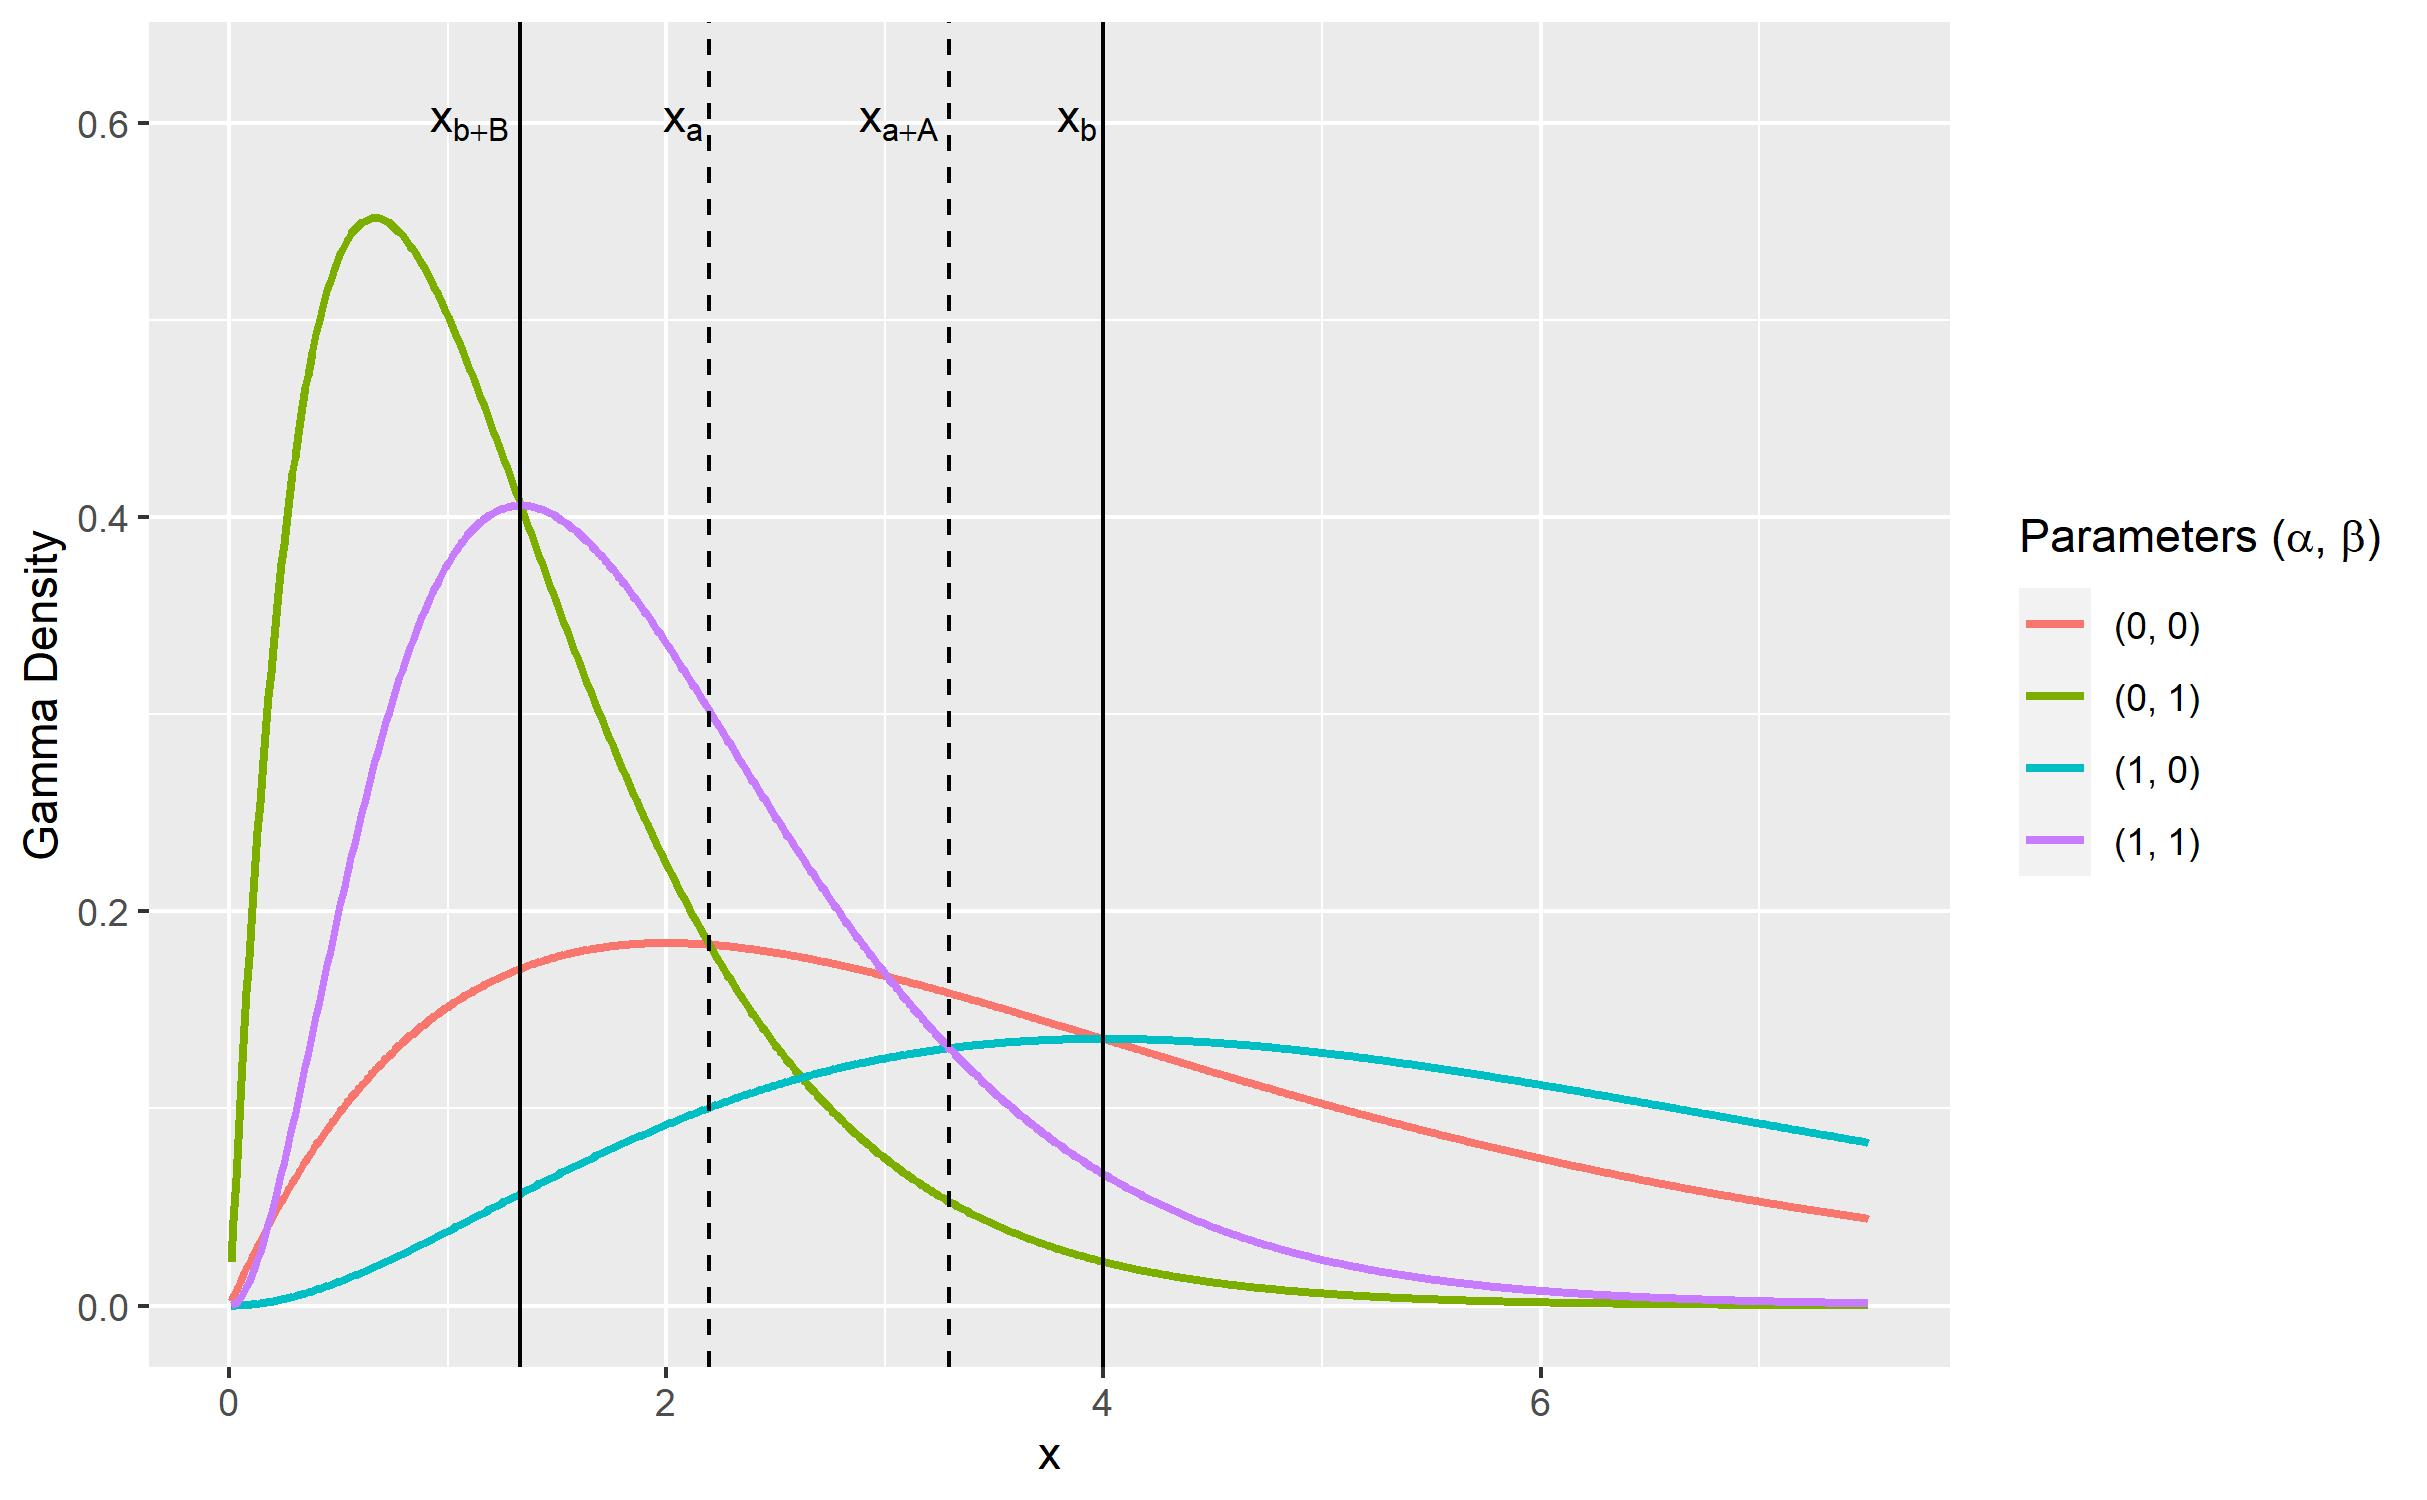
\includegraphics[width=\textwidth]{gamma_minorization_2.jpg}
		\caption{Example of minorization of the density of a gamma distribution $Ga(2+\alpha, 0.5+\beta)$ for $\alpha$ and $\beta$ jointly.}
		\label{fig:gam2}
	\end{figure}
	
	% Truncated Exponential
	Proof of Lemma \ref{pro:tru}
	
	\begin{proof}
		Remember that $\TruncExp(u; \mu, 0, u) = \frac{\mu \exp\{-u\mu\}}{1-\exp\{-u\mu\}}$ is the density of an exponential distribution bounded above by $u$.
		\begin{align*}
			\frac{d}{d\mu}\TruncExp(u; \mu, 0, u)
			& = \left(\frac{\exp\{-u\mu\}}{1-\exp\{-u\mu\}} \right) \left[ 1-\mu u - \mu u \left(\frac{\exp\{-u\mu\}}{1-\exp\{-u\mu\}} \right) \right]
		\end{align*}
		Now let $g(\mu) = 1-\mu u - \mu u \left(\frac{\exp\{-u\mu\}}{1-\exp\{-u\mu\}} \right)$. By L'H\^{o}pital's rule, $g(0) = 0$. Moreover, for $\mu>0$, we have
		\begin{align*}
			g'(\mu)
			& = - \mu \left(1+\frac{\exp\{-u\mu\}}{1-\exp\{-u\mu\}} \right) \left[ 1-u\mu \left(\frac{\exp\{-u\mu\}}{1-\exp\{-u\mu\}} \right) \right]  \\
			& = - \mu \left(1+\frac{\exp\{-u\mu\}}{1-\exp\{-u\mu\}} \right) \left[ 1- \frac{u\mu}{\exp\{u\mu\}-1} \right] \\
			& \le 0
		\end{align*}
		where the inequality follows from $\frac{u\mu}{\exp\{u\mu\}-1}\le1$.
		This implies that $g(\mu) \le 0$ for $\mu>0$. We therefore have $\frac{d}{d\mu}\TruncExp(u; \mu, 0, u) \le 0$ and the result of the proposition follows.
	\end{proof}

	
	\bibliographystyle{plain}
	\bibliography{bibliography}
	
\end{document}